% This is samplepaper.tex, a sample section demonstrating the
% LLNCS macro package for Springer Computer Science proceedings;
% Version 2.20 of 2017/10/04
%
\documentclass[runningheads]{llncs}
%
\usepackage{graphicx}
% Used for displaying a sample figure. If possible, figure files should
% be included in EPS format.
%
% If you use the hyperref package, please uncomment the following line
% to display URLs in blue roman font according to Springer's eBook style:
\usepackage{hyperref}
\renewcommand\UrlFont{\color{blue}\rmfamily}

% Added by me
\usepackage[dvipsnames]{xcolor}
\usepackage{multicol}
% \usepackage{listings}
\usepackage[frozencache,cachedir=.]{minted}
% http://tug.ctan.org/tex-archive/macros/latex/contrib/listings/listings.pdf
% \renewcommand{\ttdefault}{lmtt} % 
\usepackage{courier}
% \usepackage{seqsplit} % allow line breaking in texttt
\usepackage{latexsym}
\usepackage{amsmath,ascmac,amssymb,thmtools} 
% \theoremstyle{definition}
% \newtheorem{theorem}{Theorem}[section]
% \newtheorem{lemma}[theorem]{Lemma}
% \newtheorem{definition}[theorem]{Definition}
% \newtheorem{example}[theorem]{Example}
\usepackage{stmaryrd}
% \usepackage{comment}
\usepackage{graphicx}
\usepackage{mydef}
\usepackage[normalem]{ulem}
\usepackage{minitoc}
\usepackage{fontawesome5}

\usepackage{bcprules} % 
\usepackage{bussproofs} % 


\usepackage{tikz}
\usetikzlibrary{positioning, arrows, arrows.meta, decorations.markings, shapes.geometric, shapes.misc, fit, calc}

\definecolor{LightGray}{gray}{0.95}
\newcommand{\vlkey}[1]{\textcolor{OliveGreen}{\textbf{#1}}}

\newif\ifdraftComments
\draftCommentstrue
\def\mkDraftFn#1#2{%
  \expandafter\def\csname #1\endcsname##1{\ifdraftComments\textcolor{#2}{[#1: ##1]}\marginpar[$\longrightarrow$]{$\longleftarrow$}\fi}%
}
\mkDraftFn{YT}{red}


\setminted[haskell]{frame=lines,
% framesep=2mm,
baselinestretch=1.1,
bgcolor=LightGray,
fontsize=\footnotesize,
% linenos,
escapeinside=@@,
}

\begin{document}
%
\title{Compilation Semantics for a Programming Language with Versions}

% \titlerunning{Compilation with Versions}
% If the paper title is too long for the running head, you can set
% an abbreviated paper title here

% \author{Anonymous}
\author{Yudai Tanabe\inst{1}\orcidID{0000-0002-7990-0989} \faIcon{envelope}\and\\
Luthfan Anshar Lubis\inst{2}\orcidID{0000-0002-1498-7788} \and\\
Tomoyuki Aotani\inst{3}\orcidID{0000-0003-4538-0230} \and\\
Hidehiko Masuhara\inst{2}\orcidID{0000-0002-8837-5303}
}

\authorrunning{Y. Tanabe et al.}
% First names are abbreviated in the running head.
% If there are more than two authors, 'et al.' is used.

% \institute{Anonymous}
\institute{
Kyoto University, Kyoto, Japan
\faIcon{envelope} \footnote{\faIcon{envelope} Corresponding author}\email{yudaitnb@fos.kuis.kyoto-u.ac.jp}\\\and
Tokyo Institute of Technology, Tokyo, Japan
\email{\{luthfanlubis@prg.is.titech.ac.jp | masuhara@acm.org\}}\\\and
Sanyo-Onoda City University, Yamaguchi, Japan
\email{aotani@rs.socu.ac.jp}
}
%
\maketitle            % typeset the header of the contribution
%  
\begin{abstract}
\emph{Programming with versions} is a paradigm that allows a program to use multiple versions of a module so that the programmer can selectively use functions from both older and newer versions of a single module.
Previous work formalized \corelang{}, a core calculus for programming with versions, but it has not been integrated into practical programming languages.
In this paper, we propose \mylang{}, a Haskell-subset surface language for \corelang{} along with its compilation method.
We formally describe the core part of the \mylang{} compiler, which translates from the surface language to the core language by leveraging Girard's translation, soundly infers the consistent version of expressions along with their types, and generates a multi-version interface by bundling specific-version interfaces. 
We conduct a case study to show how \mylang{} supports practical software evolution scenarios and discuss the method's scalability.
\keywords{Type system \and Type inference \and Version control system.}
\end{abstract}
%
%
%
\section{Introduction}  \label{sec:introduction}

\newcommand\inexpIntro[3]{#1?(#2,#3).}
\newcommand\rinexpIntro[3]{*#1?(#2,#3).}
\newcommand\outexpIntro[3]{#1!(#2,#3).}
\newcommand\outatomIntro[3]{#1!(#2,#3)}

We propose a fully automated method for proving termination of \(\pi\)-calculus processes.
Although there have been a lot of studies on termination analysis for the \(\pi\)-calculus
and related calculi~\cite{Deng06IC,Demangeon07,SangiorgiTermination,KobayashiHybrid,Yoshida04IC,DBLP:journals/jlp/DemangeonHS10,Venet98SAS}, most of them have been rather theoretical,
and there have been surprisingly little efforts in developing  fully automated termination
verification methods and tools based on them. To our knowledge,
Kobayashi's \typical{}~\cite{TyPiCal,KobayashiHybrid} is the only exception that
can prove termination of \(\pi\)-calculus processes (extended with natural numbers)
fully automatically, but its termination analysis is quite limited (see Section~\ref{sec:relatedwork}).

Our method is based on a reduction to termination analysis for sequential programs:
we translate a \(\pi\)-calculus process \(P\) to a sequential program \(S_P\), so that
if \(S_P\) is terminating, so is \(P\). The reduction allows us to use
powerful, mature methods and tools
for termination analysis of sequential programs~\cite{heizmann2016ultimate,freqterm,DBLP:conf/lics/PodelskiR04,Kuwahara2014Termination,DBLP:journals/cacm/CookPR11}.

The idea of the translation is to convert a chain of communications on replicated input
channels to a chain of recursive function calls of the target sequential program.
Let us consider the following Fibonacci process:
\begin{align*}
    & \rinexpIntro{\fib}{n}{r}
        \ifexp{n<2}{ \soutatom{r}{1} \\ &\quad}
                   { \nuexp{s_1} \nuexp{s_2} (\outatomIntro{\fib}{n-1}{s_1} \PAR \outatomIntro{\fib}{n-2}{s_2} \PAR \sinexp{s_1}{x}\sinexp{s_2}{y}\soutatom{r}{x+y}) \\}
    & \PAR \outatomIntro{\fib}{m}{r}
\end{align*}
Here, the process
$\rinexpIntro{\fib}{n}{r} \ldots$ is a function server that computes the \(n\)-th Fibonacci number
in parallel and returns the result to \(r\),
and $\outatom{\fib}{m}{r}$ sends a request for computing the \(m\)-th Fibonacci number;
those who are not familiar with the syntax of the \(\pi\)-calculus may wish to consult
Section~\ref{sec:targetlanguage} first.
To prove that the process above is terminating for any integer \(m\),
it suffices to show that there is no infinite chain of communications on $\fib$:
\[
    \fib(m,r) \to \fib(m_1,r_1) \to \fib(m_2,r_2) \to \cdots.
\]
We convert the process above to the following program:\footnote{The actual translation
  given later is a little more complex.}
\begin{verbatim}
 let rec fib(n) = if n<2 then () else (fib(n-1) [] fib(n-2)) in
 fib(m)
\end{verbatim}
Here, \texttt{[]} represents the non-deterministic choice.
Note that, although the calculation of Fibonacci numbers is not preserved,
for each chain of communications on \texttt{fib}, there is a corresponding
sequence of recursive calls:
\[
\mathtt{fib}(m) \to \mathtt{fib}(m_1) \to \mathtt{fib}(m_2) \to \cdots.
\]
Thus, the termination of the sequential program above implies the termination of
the original process.
As shown in the example above, (i) each communication on a replicated input channel
is converted to a function call, (ii) each communication on a non-replicated input
channel is just removed (or, in the actual translation, replaced by a call of
a trivial function defined by \(f(\seq{x})=(\,)\)), and (iii) parallel composition
is replaced by a non-deterministic choice.
We formalize the translation outlined above and prove its correctness.

The basic translation sketched above sometimes loses too much information.
For example, consider the following process:
\begin{align*}
    & \rinexpIntro{\pre}{n}{r} \soutatom{r}{n-1} \\
    & \PAR \rinexpIntro{f}{n}{r} \ifexp{n<0}{ \soutatom{r}{1} }
                                       { \nuexp{s} (\outatomIntro{\pre}{n}{s} \PAR \sinexp{s}{x}\outatomIntro{f}{x}{r}) } \\
    & \PAR \outatomIntro{f}{m}{r}
\end{align*}
The translation sketched above would yield:
\begin{verbatim}
  let pred(n) = n-1 in
  let rec f(n) = if n<0 then () else (pred(n) [] f(*)) in
  f(m)
\end{verbatim}
Here, \texttt{*} represents a non-deterministic integer: since we have removed
the input $\sinatom{s}{x}$, we do not have information about the value of \( x \).
As a result, the sequential program above is non-terminating, although the original
process is terminating.
To remedy this problem, we also refine the basic translation above by using a refinement
type system for the \(\pi\)-calculus. Using the refinement type system,
we can infer that the value of \(x\) in the original process is less than \(n\),
so that we can refine the definition of \texttt{f} to:
\begin{verbatim}
 let rec f(n) = ... else (pred(n) [] let x=* in assume(x<n);f(x))
\end{verbatim}
The target program is now terminating, from which
we can deduce that the original process is also terminating.
We have implemented an automated tool based on the refined translation above.

The contributions of this paper are summarized as follows.
\begin{itemize}
\item The formalization of the basic translation from the \(\pi\)-calculus
  (extended with integers) to sequential programs, and a proof of its correctness.
\item The formalization of a refined translation based on a refinement type system.
\item An implementation of the refined translation, including automated refinement type
  inference based on CHC solving, and experiments to evaluate the effectiveness of
  our method.
\end{itemize}

The rest of this paper is structured as follows.
Section~\ref{sec:targetlanguage} introduces the source and target languages
of our translation.
Section~\ref{sec:approach} 
formalizes the basic translation, and proves its correctness.
Section~\ref{sec:refinement} refines the basic translation by using a refinement type system.
Section~\ref{sec:implementation} reports an implementation and experiments.
Section~\ref{sec:relatedwork} discusses related work,
and Section~\ref{sec:conclusion} concludes the paper.

\section{System Overview} \label{sec:overview}

In this section, we give an overview of our keyword search system. Our approach can be summarized as a two-phase framework, as illustrated in Figure \ref{fig:overview}. 

\begin{figure} [h]
	\centering
	\scalebox{1.0}[1.0]
	{
		\resizebox{\linewidth}{!}
		{
			\includegraphics[scale=0.5]{visio_pics/approach_overview_simp.pdf}
		}
	}
	\vspace{-0.3in}
	\caption{An Overview of Our Approach.}
	\label{fig:overview}
	\vspace{-0.2in}
\end{figure}

\subsection{Phase-I: Segmentation and Annotation} \label{sec:phase1}
The first phase is to segment the keyword token sequence $RQ = \{k_1, k_2, ..., k_m\}$ into several \emph{terms} and each term is annotated with one of the three characters $\{$entity, class, relation$\}$. The converted query is called \emph{annotated query}. Formally, we denote an \textit{annotated query} as $AQ= \{t_1:c_1, t_2:c_2, ..., t_l:c_l\}$, where each $t_i$ is a term and  $c_i \in \{$entity, class, relation$\}$. Note that the first phase (i.e., segmentation and annotation) is not the focus of this paper, as it has been studied extensively \cite{hua2015short,han2011generative, li2011faerie, nakashole2012patty,cai2013large}. We briefly describe the implementation of the first phase as follows. 

For each continuous subsequence $s$ in $RQ$, we check whether it could be matched to an entity, a class, or a relation of the RDF dataset, by employing the existing techniques of entity linking \cite{han2011generative,li2011faerie, ratinov2011local} and relation paraphrasing \cite{nakashole2012patty,cai2013large}. If $s$ is matched, we regard $s$ as a \emph{candidate term} $t_i$, and annotate it with the corresponding character (entity, class, or relation).
We may find that two candidate terms $t_i$ and $t_j$ \emph{overlap} with each other. We say $t_i$ overlaps with $t_j$ if and only if they have at least one common token. Obviously, if two terms overlap, they cannot occur at the same segmentation result. For example, ``university'' and ``university locate USA'' cannot occur in the same segmentation result. We build a \emph{candidate term graph} to describe the mutually exclusive relations: (1) each candidate term $t_i$ is represented a vertex; (2) there is an edge between $t_i$ and $t_j$ if and only of there is \emph{no} overlapping tokens between $t_i$ and $t_j$. Thus each maximal clique in the candidate term graph stands for a possible segmentation result. To obtain top-$N$ best $AQ$, we employ the maximal clique algorithm \cite{bron1973algorithm}, and adopt the pairwise metrics in \cite{hua2015short} to rank the segmentation result.
In out example, we get the top-2 $AQ$ as shown in Figure \ref{fig:overview}.

In the first phase, we have converted keyword token sequence $RQ$ into top-$N$ $AQ$ by some off the shelf techniques. Furthermore, these terms in $AQ$ have been matched to some elementary query graph building blocks (i.e., entity/class vertices and predicate edges). Specifically, if a term $t_i$ is annotated with ``entity'' or ``class'', it will be matched to candidate entity/class vertices in RDF graph.
%We do not distinguish entity vertex or class vertex until generating SPARQL, since we have the same operation on both of them.
If a term $t_i$ is annotated with ``relation'', it will be matched to a set of candidate predicates.

\vspace{-0.05in}
\begin{example}\label{example:aq}
	Given a keyword token sequence $RQ = \{$scientist, graduate, from, university, locate, USA$\}$, we obtain the annotated query $AQ=\{$``scientist'':class, ``graduate from'':relation, ``university'':class, ``locate'':relation, ``USA'':entity $\}$, where ``scientist'' is matched to $\{$dbo:Scientist$\}$, ``university'' is matched to $\{$dbo:University$\}$, ``USA'' is matched to two possible entities $\{$res:USA$\_$Today, res:United$\_$\\States$\}$ due to the ambiguity. Also, the relations ``graduate from'' and ``locate'' also match to two candidate predicates $\{$dbo:almaMater, dbo:education$\}$ and $\{$dbo:country, dbo:location$\}$
\end{example}

\vspace{-0.1in}
\subsection{Phase-II: Query Graph Assembly}
In the second phase, we concentrate on how to assemble a query graph $Q$ based on these elementary building blocks. Formally, the query graph assembly problem is defined as follows:

\vspace{-0.05in}
\begin{definition} \textbf{(Query Graph Assembly Problem)}\label{def:querygraphassembling}
	Given $n$ terms $t^{v}_i$ ($i=1,...,n$) annotated with ``entity'' or ``class'', and $m$ terms $t_j^{e}$ ($j=1,...,m$) annotated with ``relation'', each term $t^{v}_i$ is matched to a set $V_i$ of candidate entity/class vertices and each $t^{e}_j$ is matched to a set $E_j$ of candidate predicate edges. Let $\Upsilon=\{V_1, ..., V_n\}$ and $\Gamma=\{E_1, ..., E_m\}$. A valid assembly query graph is denoted as $Q (V_Q,E_Q)$, which satisfies the following constraints:
	\begin{enumerate}
		\item $|V_Q|=n$, and $\forall V_i \in \Upsilon, V_Q \cap V_i \not= \phi$; 
		\emph{/*each entity or class vertex set $V_i$ has exactly one vertex in  $Q$*/}
		\item $|E_Q|=m$, and $\forall E_j \in \Gamma, E_Q \cap E_j \not= \phi$. 
		\emph{/*each predicate edge set $E_j$ has exactly one edge in $Q$*/}
	\end{enumerate}
	Each edge $e(\langle v_1, v_2\rangle,p) \in E_Q$ connects a pair of vertices $\langle v_1, v_2\rangle \in V_Q$ by a predicate $p$.
	The assembly cost of $Q$ is
	\begin{equation} \label{equ:cost}
	cost(Q)=\sum_{e(\langle v_1, v_2\rangle,p) \in E_Q}{w(\langle v_1, v_2\rangle,p)}
	\end{equation}
	where  $w(\langle v_1, v_2\rangle,p)$ denotes the triple assembly cost. 
	
	
	The \emph{query graph assembly} (QGA for short) problem is to construct a valid graph $Q$ with the minimum assembly cost. 
\end{definition} 

%\vspace{-0.06in}

There are two aspects that should be explained for QGA.

\textbf{\emph{1. Constraints:}}
The two constraints in Definition \ref{def:querygraphassembling} mean that each term $t^{v}_i$ ($1\leq i \leq n$) only corresponds to a single entity/class vertex in $Q$. For example, although ``USA'' may match two candidate entities dbo:USA$\_$Today and dbo:United$\_$States, in the final query graph $Q$, ``USA'' only matches a single entity (dbo:United$\_$States). It is analogue for the relation term $t_j^{e}$ ($1\leq j \leq m$). 

\textbf{\emph{2. Disengaged Edges:}}
A \emph{predicate edge} $e(\langle \cdot,\cdot \rangle,p)$ (in $E_j$) does not have two fixed endpoints but its edge label is fixed to predicate $p$. Thus, a predicate edge can be also called a \emph{disengaged} edge. The triple assembly cost $w(\langle v_1, v_2\rangle,p)$ measures the goodness of assembling $\langle v_1, v_2\rangle$ and $p$ into an edge in $Q$. Then the goal of the QGA problem is to determine the endpoints of $e(\langle \cdot,\cdot \rangle,p)$ to minimize the overall $cost(Q)$.

After finding the optimal $Q$ with minimum $cost(Q)$, we can translate it to SPARQL statements naturally, as illustrated in Figure \ref{fig:overview}.

\subsection{Graph Embedding Cost Model}
Note that the triple assembly cost $w(\langle v_1, v_2\rangle,p)$ can be any positive cost function, which does not affect the hardness of QGA. In other words, the QGA problem is a general computing framework to interpret the input keywords as SPARQL, which does not depend on any specific triple assembly cost function.

\begin{figure} [b]
	\centering
	\scalebox{0.55} [0.50]
	{
		\resizebox{\linewidth}{!}
		{
			\includegraphics[scale=1.0]{visio_pics/transe_visualizing.pdf}
		}
	}
	\caption{Visualizing the Intuition of Graph Embedding.}
	\label{fig:transe_visualizing}
	\vspace{-0.2in}
\end{figure}

The only thing affected by the selection of triple assembly cost function is the system's accuracy. A good cost function can guide to assemble correct query graph $Q$ that implies users' query intention. The process of assembling $\langle v_1, v_2\rangle$ and $p$ into a triple is analogue to ``link prediction'' problem in the RDF knowledge graph \cite{miller2009nonparametric}. Given two entity/class vertices $v_1$ and $v_2$, the link prediction is to ``predict'' the predicate $p$ between $v_1$ and $v_2$, and $w(\langle v_1,v_2\rangle, p)$ is a \emph{measure} of the prediction. Recent research show that the graph embedding technique is superior to other traditional approaches, such as \cite{miller2009nonparametric,nickel2011three,jenatton2012latent}. In the graph embedding model, all subjects (s), objects (o) and predicates (p) are encoded as multi-dimensional vectors $\overrightarrow{s}$, $\overrightarrow{p}$ and $\overrightarrow{o}$ such that $\overrightarrow s  + \overrightarrow p  \approx \overrightarrow o $ if $\langle s,p,o \rangle \in G$ (i.e., $\langle s,p,o\rangle$ is a triple in RDF graph); while $\overrightarrow s  + \overrightarrow p$ should be far away from $\overrightarrow o$ otherwise. Figure \ref{fig:transe_visualizing} visualizes the intuition. From the intuition, the structural information among entities, classes and relations in RDF graph is embedded into vectors. Therefore, we define the triple assembly cost based on graph embedding vectors as follows.


\begin{definition}\textbf{ (Triple Assembly Cost) }. \label{def:tripleassemblycost}
	Given two entity/class vertices $v_1$ and $v_2$ and a predicate edge $p$, the \emph{cost} of assembly triple $(v_1,p,v_2)$ is denoted as follows:
	\begin{equation}\label{equ:tripleassembly}
	w(\langle v_1, v_2\rangle, p) = MIN(| \overrightarrow{v_1} + \overrightarrow p  - \overrightarrow {v_2 } |, | \overrightarrow{v_2} + \overrightarrow p  - \overrightarrow {v_1 } |)
	\end{equation}
	where $\overrightarrow{v_1}$, $\overrightarrow {v_2}$ and $\overrightarrow {p}$ are the encoded multi-dimensional vectors  of $v_1$, $v_2$ and $p$, respectively. 
	%where $|x|_+$ denotes the positive part of $x$. 
\end{definition}  

\begin{figure} [h]
	\centering
	\scalebox{1.0}
	{
		\resizebox{\linewidth}{!}
		{
			\includegraphics[scale=1.0]{visio_pics/query_graph_elements_example2.pdf}
		}
	}
%	\caption{Candidate Entity/Class Vertices and Predicate Edges.}
	\caption{Elementary Query Graph Building Blocks.}
	\label{fig:graph_elements_exp2}
	\vspace{-0.3in}
\end{figure}

\begin{figure} [h]
	\newcommand{\mywidth}{0.23\textwidth}
	\centering
	\begin{subfigure}[t]{\mywidth}
		\centering
		\resizebox{\linewidth}{!}
		{
			\includegraphics{visio_pics/query_assembly_graph_q1.pdf}
			
		}
		\caption{$cost(Q_1)=1.76$}
		\label{fig:assembly_query_graph_q1}
	\end{subfigure}
	\begin{subfigure}[t]{\mywidth}
		\centering
		\resizebox{1.0\linewidth}{!}
		{
			\includegraphics{visio_pics/query_assembly_graph_q2.pdf}
		}
		\caption[font=\small]{$cost(Q_2)=2.46$}
		%        \vspace{0.1in}
		\label{fig:assembly_query_graph_q2}
	\end{subfigure}
	\caption{Possible Assembly Query Graphs.}
	%    \vspace{-0.1in}
	\label{fig:assembly_query_graph}
	\vspace{-0.1in}
\end{figure}

\begin{example} In our example, there are three entity/class terms ``scientist'', ``university'', ``USA'' and two relation terms ``graduate from''  and ``locate''. Their corresponding entity/class vertices and predicate edges are shown in Figure \ref{fig:graph_elements_exp2}. There are two different assembly query graph $Q_1$ and $Q_2$ in Figure \ref{fig:assembly_query_graph}, among which $cost(Q_1)<cost(Q_2)$. Thus, the QGA problem result is $Q_1$ (Figure \ref{fig:assembly_query_graph_q1}).
%It means that we interpret the keywords as a query graph $Q$ and evaluate $Q$ using SPARQL query engine to return answers to users. 
\end{example} 
% Section Template

\section{Compilation} % Main Section title
\label{compilation} % Change X to a consecutive number; for referencing this Section elsewhere, use \ref{SectionX}

\begin{figure}[tb]
\centering
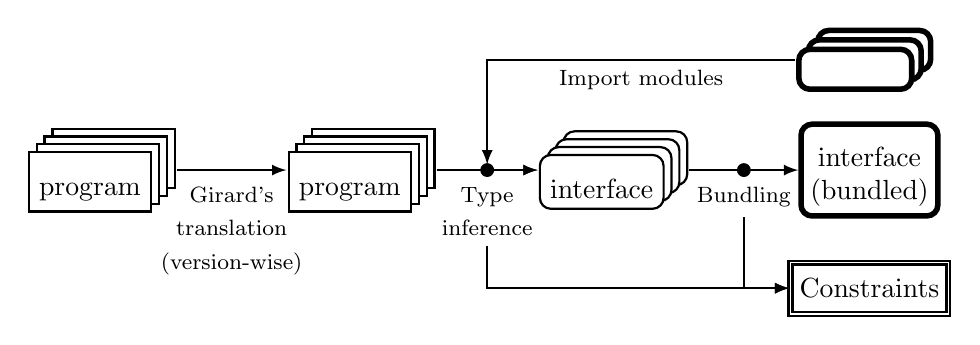
\begin{tikzpicture}[thick]
    \tikzset{vecArrow/.style={thick, decoration={markings,mark=at position
    1 with {\arrow[semithick]{open triangle 60}}},
    double distance=1.4pt, shorten >= 5.5pt,
    preaction = {decorate},
    postaction = {draw,line width=1.4pt, white,shorten >= 4.5pt}}};
    \tikzset{innerWhite/.style={semithick, white,line width=1.4pt, shorten >= 4.5pt}};
    \tikzset{Package/.style={rectangle, fill=cyan!10, text centered, rounded corners, minimum width=1.9cm, minimum height=0.65cm}};
    \tikzset{App/.style={rectangle, text centered, minimum width=1.2cm, minimum height=0.65cm}};

    \newlength\mywidth
    \newlength\myheight
    \newlength\tempdimen
    
    \newcommand\getdimensions[1]{
        \pgfextractx{\mywidth}{\pgfpointanchor{#1}{east}}
        \pgfextractx{\tempdimen}{\pgfpointanchor{#1}{west}}
        \addtolength{\mywidth}{-\tempdimen}
        \pgfextracty{\myheight}{\pgfpointanchor{#1}{north}}
        \pgfextracty{\tempdimen}{\pgfpointanchor{#1}{south}}
        \addtolength{\myheight}{-\tempdimen}
    }

    \tikzset{
      pics/stacked rectangles/.style n args={4}{
        code={
          \def\rectangleWidth{2cm}  % 長方形の幅を固定
          \def\rectangleHeight{1cm} % 長方形の高さを固定
          \pgfmathsetmacro\offsetY{(#1+1)*#2/2} % Yのオフセットを計算
          
          % 一時的なrect1を描画してサイズを取得
          \node[draw=none, align=center] (tempRect1) at (1*#2,1*#2-\offsetY) { #3 };
          
          % ここでtempRect1の寸法を取得
          \getdimensions{tempRect1}
          
          % 長方形を描画
          \foreach \i in {#1,...,2} {
            \node[draw, fill=white, minimum width=\mywidth, minimum height=\myheight] (rect\i) at (\i*#2,\i*#2-\offsetY) {};
          }

          % 一番前の長方形を描画
          \node[draw, fill=white, minimum width=\mywidth, minimum height=\myheight, align=center] (rect1) at (1*#2,1*#2-\offsetY) { #3 };
    
          % すべての長方形を囲む仮想的なノード
          \node[draw=none, inner sep=0pt, fit={(rect1.south west) (rect#1.north east)}, name=#4] {};
        }
      }
    }

    \tikzset{
      pics/stackedty rectangles/.style n args={4}{
        code={
          \def\rectangleWidth{2cm}  % 長方形の幅を固定
          \def\rectangleHeight{1cm} % 長方形の高さを固定
          \pgfmathsetmacro\offsetY{(#1+1)*#2/2} % Yのオフセットを計算
          
          % 一時的なrect1を描画してサイズを取得
          \node[draw=none, align=center] (tempRect1) at (1*#2,1*#2-\offsetY) { #3 };
          
          % ここでtempRect1の寸法を取得
          \getdimensions{tempRect1}
          
          % 長方形を描画
          \foreach \i in {#1,...,2} {
            \node[draw, fill=white, minimum width=\mywidth, minimum height=\myheight, rounded corners] (rect\i) at (\i*#2,\i*#2-\offsetY) {};
          }

          % 一番前の長方形を描画
          \node[draw, fill=white, minimum width=\mywidth, minimum height=\myheight, align=center, rounded corners] (rect1) at (1*#2,1*#2-\offsetY) { #3 };
    
          % すべての長方形を囲む仮想的なノード
          \node[draw=none, inner sep=0pt, fit={(rect1.south west) (rect#1.north east)}, name=#4] {};
        }
      }
    }


    \tikzset{
      pics/stackedtybundled rectangles/.style n args={4}{
        code={
          \def\rectangleWidth{2cm}  % 長方形の幅を固定
          \def\rectangleHeight{1cm} % 長方形の高さを固定
          \pgfmathsetmacro\offsetY{(#1+1)*#2/2} % Yのオフセットを計算
          
          % 一時的なrect1を描画してサイズを取得
          \node[draw=none, align=center] (tempRect1) at (1*#2,1*#2-\offsetY) { #3 };
          
          % ここでtempRect1の寸法を取得
          \getdimensions{tempRect1}
          
          % 長方形を描画
          \foreach \i in {#1,...,2} {
            \node[draw, fill=white, minimum width=\mywidth, minimum height=\myheight, rounded corners, line width=2pt] (rect\i) at (\i*#2,\i*#2-\offsetY) {};
          }

          % 一番前の長方形を描画
          \node[draw, fill=white, minimum width=\mywidth, minimum height=\myheight, align=center, rounded corners, line width=2pt] (rect1) at (1*#2,1*#2-\offsetY) { #3 };
    
          % すべての長方形を囲む仮想的なノード
          \node[draw=none, inner sep=0pt, fit={(rect1.south west) (rect#1.north east)}, name=#4] {};
        }
      }
    }

    \pic at (0,0) {stacked rectangles={4}{0.1cm}{\mylang{}\\program}{vl1}};
    % \node[draw,App, align=center] at (3.0,0) (vlmini1) {\vlmini{}\\($V_{M_i}$)};
    \pic at (3.3,0) {stacked rectangles={4}{0.1cm}{\vlmini{}\\program}{vlmini1}};
    % \node[draw,App, align=center] at (6.0,0) (vlmini2) {\vlmini{}\\interface};
    \pic at (6.5,0) {stackedty rectangles={4}{0.1cm}{\vlmini{}\\interface}{vlmini2}};
    \pic at (9.7,1.4) {stackedtybundled rectangles={3}{0.12cm}{\vphantom{b}\hspace{3em}}{vlmini4}};
    \node[draw,App, align=center, rounded corners, line width=2pt] at (10,0) (vlmini3) {\vlmini{}\\interface\\(bundled)};
    % \node[draw,App, align=center, rounded corners, line width=2pt, minimum width=1.62cm, minimum height=0.5cm] at (10,1.4) (vlmini4) {};
    \coordinate (topofinference) at ($(vlmini1.east)!0.5!(vlmini2.west)$);
    \coordinate (botofinference) at ($(vlmini1.east)!0.5!(vlmini2.west) + (0, -1.75)$);
    \coordinate (topofbundling) at ($(vlmini2.east)!0.5!(vlmini3.west)$);
    \coordinate (botofbundling) at ($(vlmini2.east)!0.5!(vlmini3.west) + (0, -1.75)$);
    % \node[draw,App,double,align=center] at (botofinference) (vdep) {\footnotesize{Variable}\\\footnotesize{dependency}};
    % \node[draw,App,double,align=center] at (botofbundling) (ldep) {\footnotesize{Label}\\\footnotesize{dependency}};
    \node[draw,App,double] at (10,-1.5) (constraints) {Constraints};
    \fill (topofinference) circle (2.5pt);
    \fill (topofbundling) circle (2.5pt);
    
    \draw[-latex] (vl1.east) to [yshift=-5]node[midway,below,align=center] {\footnotesize{Girard's}\\\footnotesize{translation}\\\footnotesize{(version-wise)}} (vlmini1.west);
    \draw[-latex] (vlmini1.east) to node[midway,below] {} (vlmini2.west);
    \draw[-latex] (vlmini1.east) to [yshift=-5]node[midway,below,align=center] (inference){\footnotesize{Type}\\\footnotesize{inference}} (vlmini2.west);
    \draw[-latex] (vlmini2.east) to [yshift=-5]node[midway,below,align=center] (bundling) {\footnotesize{Bundling}} (vlmini3.west);
    \draw[-latex] (vlmini4.west) -| node[near start,below,align=center] {\footnotesize{Import modules}} ([yshift=2]topofinference);
    \draw[-latex] (inference.south) |- (constraints.west);
    \draw[-latex] (bundling.south) |- (constraints.west);
    % \draw[-latex] (inference.south) -- (vdep.north);
    % \draw[-latex] (bundling.south) -- (ldep.north);
\end{tikzpicture}
\caption{The translation phases for a single module with multiple versions.}
\label{fig:translationoverview}
\end{figure}
The entire translation consists of three parts: (1) \emph{Girard's translation}, (2) an \emph{algorithmic type inference}, and (3) \emph{bundling}.
Figure \ref{fig:translationoverview} shows the translation process of a single module. First, through Girard's translation, each version of the \mylang{} program undergoes a version-wise translation into the \vlmini{} program. 
Second, the type inference synthesizes types and constraints for top-level symbols. Variables imported from external modules reference the bundled interface generated in the subsequent step.
Finally, to make the external variables act as multi-version expressions, bundling consolidates each version's interface into one \vlmini{} interface.
These translations are carried out in order from downstream of the dependency tree.
By resolving all constraints up to the main module, the appropriate version for every external variable is determined.

It is essential to note that the translations focus on generating constraints for dispatching external variables into version-specific code. While implementing versioned records in \corelang{} presents challenges, such as handling many version labels and their code clones, our method is a constraint-based approach in \vlmini{} that enables static inference of version labels without their explicit declaration.

In the context of coeffect languages, constraint generation in \mylang{} can be seen as the automatic generation of type declarations paired with resource constraints.
Granule\cite{Orchard:2019:Granule} can handle various resources as coeffects, but it requires type declarations to indicate resource constraints. \mylang{} restricts its resources solely to the version label set. This specialization enables the automatic collection of version information from external sources outside the codebase.

\subsection{An Intermediate Language, \vlmini{}}
% \vspace{-1\baselineskip}
\subsubsection{Syntax of \vlmini{}}
\begin{figure}[tb]
    \hrule
    \medskip
    \begin{minipage}{.9\textwidth}
        \textbf{\vlmini{} syntax (w/o data constructors and version control terms)}
    \end{minipage}
    \begin{minipage}{\textwidth}
        \vspace{-.8\baselineskip}
        \begin{minipage}{.475\textwidth}
          \begin{align*}
            t & ::= n \mid x \mid \app{t_1}{t_2} \mid \lam{p}{t} \mid \pr{t} \tag{terms}\\
            p & ::= x \mid [x] \tag{patterns}\\
            A, B & ::= \inttype{} \mid \alpha \mid \ftype{A}{B} \mid \vertype{r}{A} \tag{types}\\
            \kappa & ::= \typekind{} \mid \labelskind{} \tag{kinds}
          \end{align*}
        \end{minipage}
        \begin{minipage}{.475\textwidth}
          \begin{align*}
            \Gamma & ::= \emptyset \mid \Gamma, x:A \mid \Gamma, x:\verctype{A}{r} \tag{contexts}\\
            \Sigma & ::= \emptyset \mid \Sigma, \alpha:\kappa \tag{type variable kinds}\\
            R      & ::= - \mid r \tag{resource contexts}\\
          \end{align*}
        \end{minipage}
    \end{minipage}
    \begin{minipage}{.9\textwidth}
        \medskip\textbf{Extended with data constructors}
    \end{minipage}
    \begin{minipage}{\textwidth}
        \vspace{-.5\baselineskip}
        \begin{minipage}{.52\textwidth}
          \begin{align*}
            t & ::= \ldots \mid C\,\overline{t_i} \mid \caseof{t}{\overline{p_i \mapsto t_i}}\tag{terms}\\
            p & ::= \ldots \mid C\,\overline{p_i} \tag{patterns}\\
            C & ::= (,) \mid [,] \tag{constructors}
          \end{align*}
        \end{minipage}
        \begin{minipage}{.44\textwidth}
          \begin{align*}
            A, B & ::= ... \mid K \overline{A_i} \tag{types}\\
            K    & ::= (,) \mid [,] \tag{type constructors}\\
          \end{align*}
        \end{minipage}
    \end{minipage}
    \begin{minipage}{.9\textwidth}
        \medskip\textbf{Extended with version control terms}
    \end{minipage}
    \begin{minipage}{\textwidth}
        \vspace{-.5\baselineskip}
        \begin{minipage}{\textwidth}
          \begin{align*}
            t & ::= \ldots \mid \verof{\{\overline{M_i=V_i}\}}{t} \mid \unver{t}\hspace{6em}\tag{terms}
          \end{align*}
        \end{minipage}
    \end{minipage}
    \begin{minipage}{.9\textwidth}
        \medskip\textbf{\vlmini{} constraints}
    \end{minipage}
    \begin{minipage}{\textwidth}
      \vspace{-.5\baselineskip}
      \begin{align*}
        \mathcal{C} & ::= \underbrace{\top \mid \mathcal{C}_1 \land \mathcal{C}_2 \mid \mathcal{C}_1 \lor \mathcal{C}_2}_{\substack{\text{propositional}\\\text{formulae}}} \mid \underbrace{\vphantom{\mid}\alpha \preceq \alpha'}_{\substack{\text{variable}\\\text{dependencies}}} \mid \underbrace{\vphantom{\mid}\alpha \preceq \mathcal{D}}_{\substack{\text{label}\\\text{dependencies}}}\tag{dependency 
 constraints}\\
        \mathcal{D} & ::= \cs{\overline{M_i = V_i}} \tag{dependent labels}\\
        \Theta      & ::= \top \mid \Theta_1 \land \Theta_2 \mid \{A \sim B\} \tag{type constraints}
      \end{align*}
    \end{minipage}
  % \begin{align*}
  %   t & ::= n \mid x \mid \app{t_1}{t_2} \mid \lam{p}{t} \mid \pr{t} \mid C\,\overline{t_i} \mid \caseof{t}{\overline{p_i \mapsto t_i}}\tag{terms}\\
  %   p & ::= n \mid x \mid \_ \mid [p] \mid C\,\overline{p_i} \tag{patterns}\\
  %   C & ::= (,) \mid [,] \tag{constructors}\\
  %   A, B & ::= \inttype{} \mid K \overline{A_i} \mid \bgr{\alpha} \mid \ftype{A}{B} \mid \vertype{r}{A} \tag{types}\\
  %   K    & ::= (,) \mid [,] \tag{type constructors}\\
  %   \kappa & ::= \typekind{} \mid \labelskind{} \tag{kinds}\\
  %   \Gamma & ::= \emptyset \mid \Gamma, x:A \mid \Gamma, x:\verctype{A}{r} \tag{contexts}\\
  %   \Sigma & ::= \emptyset \mid \Sigma, \alpha:\kappa \tag{type variable kinds}\\
  %   R      & ::= - \mid r \tag{resource contexts}\\
  %   \mathcal{C} & ::= \top \mid \mathcal{C}_1 \land \mathcal{C}_2 \mid \mathcal{C}_1 \lor \mathcal{C}_2 \mid \underbrace{\vphantom{\mid}\alpha \preceq \alpha'}_{\textnormal{variable dependencies}} \mid \underbrace{\vphantom{\mid}\alpha \preceq L}_{\textnormal{label dependencies}}\tag{constraints}\\
  %   L & ::= \cs{\overline{M_i \mapsto V_i}} \tag{dependent labels}
  % \end{align*}
  \medskip
  \hrule
  \caption{The syntax of \vlmini{}.}
  \label{syntax:vlmini}
\end{figure}
Figure \ref{syntax:vlmini} shows the syntax of \vlmini{}.
\vlmini{} encompasses all the terms in \corelang{} except for versioned records $\nvval{l_i=t_i}$, intermediate term $\ivval{\overline{l_i=t_i}}{l_k}$, and extractions $t.l_k$. As a result, its terms are analogous to those in \lrpcf{}\cite{brunel_core_2014} and GrMini\cite{Orchard:2019:Granule}. However, \vlmini{} is specialized to treat version resources as coeffects.
We also introduce data constructors by introduction $C\,t_1,...,t_n$ and elimination $\caseof{t}{\overline{p_i \mapsto t_i}}$ for lists and pairs, and version control terms \unver{t} and \verof{\{\overline{M_i=V_i}\}}{t}. 
Here, contextual-let in \corelang{} is a syntax sugar of lambda abstraction applied to a promoted pattern.
\begin{align*}
\clet{x}{t_1}{t_2} \triangleq \app{(\lam{\pr{x}}{t_2})}{t_1}
\end{align*}

Types, version labels, and version resources are almost the same as \corelang{}.
Type constructors are also added to the type in response to the \vlmini{} term having a data constructor.
The remaining difference from \corelang{} is type variables $\alpha$. Since \vlmini{} is a monomorphic language, type variables act as unification variables; type variables are introduced during the type inference and are expected to be either concrete types or a set of version labels as a result of constraint resolution.
To distinguish those two kinds of type variables, we introduce kinds $\kappa$.
The kind \labelskind{} is given to type variables that can take a set of labels $\{\overline{l_i}\}$ and is used to distinguish them from those of kind \typekind{} during algorithmic type inference.

% \vspace{-1\baselineskip}
\subsubsection{Constraints}
% \subsection{Constraints}

In many trajectory optimization problems, there are constraints on the trajectory. It should be noted that these are different than a simple bound on the system input or state. In walking robots, common constraints are: 

\begin{itemize}
	\item reaction forces in friction cone
	\item robot above the ground
	\item robot moving forward
	\item foot hits ground from above... 
\end{itemize}

The most important thing to notice about constraints is that they must also be consistent and smooth. It isn't enough to say ``The lowest point of the foot during the step must be above the ground'' because this will pass data from a different grid-point on each function call. Rather, you need to say ``Every point of the foot trajectory must be above the ground'' (or use some very fancy smoothing in your maximization function). All rules that apply to objective functions regarding smoothness and consistency, also should be applied to calculations of constraints.

\par It is also important to minimize the number of unused constraints, provided that the problem remains smooth and consistent. One way to do this is to leave all of the constraints active, and then as you refine the solution, remove the constraints that are not being actively used. At the end of each run, check to make sure that the solution still satisfies the constraints.


The lower part of Figure \ref{syntax:vlmini} shows constraints generated through bundling and type inference.
Dependency constraints comprise \emph{variable dependencies} and \emph{label dependencies} in addition to propositional formulae.
Variable dependencies $\alpha \sqsubseteq \alpha'$ require that if a version label for $\alpha'$ expects a specific version for a module, then $\alpha$ also expects the same version.
Similarly, label dependencies $\alpha \preceq \cs{\overline{M_i = V_i}}$ require that a version label expected for $\alpha$ must be $V_i$ for $M_i$. For example, assuming that versions $1.0.0$ and $2.0.0$ exist for both modules \mn{A} and \mn{B}, the minimal upper bound set of version labels satisfying $\alpha \preceq \cs{\mn{A}\mapsto 1.0.0}$ is $\alpha = \{\{\mn{A}=1.0.0,\mn{B}=1.0.0\},\{\mn{A}=1.0.0,\mn{B}=2.0.0\}\}$. If the constraint resolution is successful, $\alpha$ will be specialized with either of two labels.
$\Theta$ is a set of type equations resolved by the type unification.

\subsection{Girard's Translation for \vlmini{}}
\label{sec:VLMini}
We extend Girard's translation between \mylang{} (lambda calculus) to \vlmini{} following Orchard's approach~\cite{Orchard:2019:Granule}.
\begin{align*}
\llbracket n \rrbracket \equiv n \qquad
\llbracket x \rrbracket \equiv x \qquad
\llbracket \lam{x}{t} \rrbracket \equiv \lam{[x]}{\llbracket t \rrbracket} \qquad
\llbracket t\ s\rrbracket \equiv \llbracket t\rrbracket\ [ \llbracket s \rrbracket ]
\end{align*}

The translation replaces lambda abstractions and function applications of \mylang{} by lambda abstraction with promoted pattern and promotion of \vlmini{}, respectively. From the aspect of types, this translation replaces all occurrences of $\ftype{A}{B}$ with $\ftype{\vertype{r}{A}}{B}$ with a version resource $r$.
This translation inserts a syntactic annotation $[*]$ at each location where a version resource needs to be addressed. Subsequent type inference will compute the resource at the specified location and produce constraints to ensure version consistency at that point.

The original Girard's translation~\cite{girardlinear1987} is well-known as a translation between the simply-typed $\lambda $-calculus and an intuitionistic linear calculus. The approach involves replacing every intuitionistic arrow $A \rightarrow B$ with $!A \multimap B$, and subsequently unboxing via let-in abstraction and promoting during application \cite{Orchard:2019:Granule}.













\subsection{Bundling}
\label{sec:bundling}
Bundling produces an interface encompassing types and versions from every module version, allowing top-level symbols to act as multi-version expressions. During this process, bundling reviews interfaces from across module versions, identifies symbols with the same names and types after removing $\square_r$ using Girard's transformation, and treats them as multiple versions of a singular symbol (also discussed in Section \ref{sec:typeincompatibilities}). In a constraint-based approach, bundling integrates label dependencies derived from module versions, ensuring they align with the version information in the typing rule for versioned records of \corelang{}.

For example, assuming that the $\mathit{id}$ that takes an \inttype{} value as an argument is available in version 1.0.0 and 2.0.0 of \mn{M} as follows:
\begin{align*}
\mathit{id} &: \vertype{\alpha_1}{(\ftype{\vertype{\alpha_2}{\inttype}}{\inttype})}\ |\ \mathcal{C}_1 \tag{\textnormal{version 1.0.0}}\\
\mathit{id} &: \vertype{\beta_1}{(\ftype{\vertype{\beta_2}{\inttype}}{\inttype})}\ |\ \mathcal{C}_2 \tag{\textnormal{version 2.0.0}}
\end{align*}
where $\alpha_1$ and $\alpha_2$ are version resource variables given from type inference. They capture the version resources of $\mathit{id}$ and its argument value in version 1.0.0. $\mathcal{C}_1$ is the constraints that resource variables of version 1.0.0 will satisfy. Likewise for $\beta_1$, $\beta_2$, and $\mathcal{C}_2$.
Since the types of $\mathit{id}$ in both versions become $\ftype{\inttype}{\inttype}$ via Girard's translation, they can be bundled as follows:
\begin{align*}
\mathit{id} : \vertype{\gamma_1}{(\ftype{\vertype{\gamma_2}{\textsf{Int}}}{\textsf{Int}})}\ |\
\mathcal{C}_1 \land \mathcal{C}_2 \land \Bigl(\ 
     &(\gamma_1 \preceq \cs{\mn{M} = 1.0.0} \land \gamma_1 \preceq \alpha_1 \land \gamma_2 \preceq \alpha_2)\\
\lor\ &(\gamma_1 \preceq \cs{\mn{M} = 2.0.0} \land \gamma_1 \preceq \beta_1 \land \gamma_2 \preceq \beta_2)\ \Bigr)
\end{align*}
where $\gamma_1$ and $\gamma_2$ are introduced by this conversion for the bundled $id$ interface, with label and variable dependencies that they will satisfy.
$\gamma_1$ captures the version resource of the bundled $\mathit{id}$. The generated label dependencies $\gamma_1 \preceq \cs{\mn{M} = 1.0.0}$ and $\gamma_1 \preceq \cs{\mn{M} = 2.0.0}$ indicate that $\mathit{id}$ is available in either version 1.0.0 or 2.0.0 of \mn{M}.
These label dependencies are exclusively\footnote{In the type checking rules for $\verof{l}{t}$, type inference exceptionally generates label dependencies. Please see Appendix \ref{appendix:vlmini_version_control_terms}} generated during bundling.
The other new variable dependencies indicate that the $\mathit{id}$ bundled interface depends on one of the two version interfaces. The dependency is made apparent by pairing the new resource variables with their respective version resource variable for each version.
These constraints are retained globally, and the type definition of the bundled interface is used for type-checking modules importing $\mathit{id}$. 

 
\section{Algorithmic Type Inference}
\label{inference}
\begin{figure*}[t]
  \centering
  \hrule
  \smallskip
  \begin{tabular}{c}
    \begin{minipage}{.9\linewidth{}}
        \textbf{\vlmini{} pattern type synthesis \ \ \ 
        \fbox{\ensuremath{\Sigma, R\,\vdash\, p : A \rhd \Gamma; \Sigma'; \Theta; \mathcal{C}}}}
    \end{minipage}
    \smallskip\\
    % \begin{minipage}{.55\linewidth}
    %   \infrule[\mbox{[}p\_\mbox{]}]{
    %     \Sigma \,\vdash\, r : \textsf{Labels}
    %     \andalso
    %     \Sigma \,\vdash\, A : \textsf{Type}\\
    %   }{
    %     \Sigma; r \,\vdash\, \_ : A \rhd \emptyset; \Sigma; \emptyset
    %   }
    % \end{minipage}
    % \\\\
    % \begin{minipage}{.45\linewidth}
    %   \infrule[pInt]{
    %     \\
    %   }{
    %     \Sigma; - \,\vdash\, n : \inttype \rhd \emptyset; \Sigma; \emptyset
    %   }
    % \end{minipage}
    % \begin{minipage}{.50\linewidth}
    %   \infrule[\mbox{[}pInt\mbox{]}]{
    %     \Sigma \,\vdash\, r : \textsf{Labels}
    %   }{
    %     \Sigma; r \,\vdash\, n : \inttype \rhd \emptyset; \Sigma; \emptyset
    %   }
    % \end{minipage}
    % \\\\
    \begin{minipage}{.475\linewidth}
      \infrule[pVar]{
        % \vdash \Sigma
        % \andalso
        % \Sigma \vdash A : \textsf{Type}
        \\
      }{
        \Sigma; - \vdash x : A \rhd x:A; \Sigma; \top; \top
      }
    \end{minipage}
    \begin{minipage}{.475\linewidth}
      \infrule[\mbox{[}pVar\mbox{]}]{
        % \vdash \Sigma
        % \andalso
        % \Sigma \vdash A : \textsf{Type}
        % \andalso
        % \Sigma \vdash r : \textsf{Labels}
        \\
      }{
        \Sigma; r \vdash x : A \rhd x:\verctype{A}{r}; \Sigma; \top; \top
      }
    \end{minipage}
    \smallskip\\
    \begin{minipage}{.85\linewidth}
      \infrule[p$\square$]{
        \Sigma, \alpha:\textsf{Labels}, \beta:\textsf{Type}; \alpha \vdash x : \beta \rhd \Delta; \Sigma'; \Theta; \mathcal{C}
      }{
        \Sigma; - \vdash [x] : A \rhd \Delta; \Sigma'; \Theta \land \{A \sim \vertype{\alpha}{\beta}\}; \mathcal{C}
      }
    \end{minipage}
    % \smallskip\\
    % \begin{minipage}{.85\linewidth}
    %   \infrule[\mbox{[}p$\square$\mbox{]}]{
    %     \Sigma, \alpha:\textsf{Labels}, \beta:\textsf{Type}; r \otimes \alpha \vdash p : \beta \rhd \Delta; \Sigma'; \Theta; \mathcal{C}
    %     % \textsf{flatten}(r,R,r',R')=(s,S)
    %   }{
    %     \Sigma; r \vdash [p] : A \rhd \Delta; \Sigma'; \Theta\land \{A \sim \vertype{\alpha}{\beta}\}; \mathcal{C}
    %   }
    % \end{minipage}
  \end{tabular}
  \smallskip
  \hrule
  \smallskip
  \begin{tabular}{c}
    \begin{minipage}{.9\linewidth{}}
        \textbf{\vlmini{} type synthesis (excerpt) \ \ \ \fbox{\ensuremath{\Sigma;\Gamma \vdash t \Rightarrow A;\Sigma';\Theta; \mathcal{C}}}}
    \end{minipage}
    \smallskip\\
    % \begin{minipage}{.95\linewidth}
    %   \infrule[$\Rightarrow_{\textsc{int}}$]{
    %     \\% \\
    %   }{
    %     \Sigma; \Gamma \vdash n \Rightarrow \textsf{Int}; \Sigma; \emptyset; \top
    %   }
    % \end{minipage}
    % \\\\
    \begin{minipage}{.45\linewidth}
      \infrule[$\Rightarrow_{\textsc{lin}}$]{
        % \vdash \Sigma
        % \andalso
        % \Sigma \vdash \Gamma
        % \andalso
        x:A\in\Gamma
      }{
        \Sigma; \Gamma \vdash x \Rightarrow A; \Sigma; x:A; \top; \top
      }
    \end{minipage}
    \begin{minipage}{.45\linewidth}
      \infrule[$\Rightarrow_{\textsc{gr}}$]{
        % \vdash \Sigma
        % \andalso
        % \Sigma \vdash \Gamma
        % \andalso
        x:\verctype{A}{r}\in\Gamma
      }{
        \Sigma; \Gamma \vdash x \Rightarrow A; \Sigma; x:\verctype{A}{1}; \top; \top
      }
    \end{minipage}
    \medskip\\
    \begin{minipage}{.95\linewidth}
      \infrule[$\Rightarrow_{\textsc{abs}}$]{
        \Sigma_1, \alpha:\textsf{Type};- \vdash p:\alpha \rhd \Gamma'; \Sigma_2; \Theta_1
        \andalso
        \Sigma_2;\Gamma,\Gamma' \vdash t \Rightarrow B;\Sigma_3;\Delta; \Theta_2; \mathcal{C}
      }{
        \Sigma_1;\Gamma \vdash \lam{p}{t} \Rightarrow \ftype{\alpha}{B};\Sigma_3;\Delta\backslash\Gamma' ; \Theta_1\land\Theta_2; \mathcal{C}
      }
    \end{minipage}
    \medskip\\
    % \begin{minipage}{.95\linewidth}
    %   \infrule[$\Rightarrow_{\textsc{app}}$]{
    %     \Sigma_1; \Gamma \vdash t_1 \Rightarrow A ; \Sigma_2; \theta_1; \mathcal{C}_1
    %     \andalso
    %     \Sigma_2; \Gamma \vdash t_2 \Rightarrow A'; \Sigma_3; \theta_2; \mathcal{C}_2
    %     \andalso\\
    %     \Sigma_4 = \Sigma_3, \beta:_{\exists}\typekind
    %     \andalso
    %     \Sigma_4 \vdash A \sim \ftype{A'}{\beta} \rhd \theta_3
    %     \andalso
    %     \theta_4 = \theta_1 \uplus \theta_2 \uplus \theta_3
    %   }{
    %     \Sigma_1;\Gamma \vdash \app{t_1}{t_2} \Rightarrow \theta_4 \beta; \Sigma_4; \theta_4; \mathcal{C}_1 \land \mathcal{C}_2
    %   }
    % \end{minipage}
    % \\\\
    \begin{minipage}{.95\linewidth}
      \infrule[$\Rightarrow_{\textsc{pr}}$]{
        \Sigma_1 \vdash [\Gamma\cap\textsf{FV}(t)]_{\textsf{Labels}} \rhd \Gamma'
        \andalso
        \Sigma_1; \Gamma' \vdash t \Rightarrow A; \Sigma_2; \Delta; \Theta; \mathcal{C}_1
        \andalso\\
        \Sigma_3 = \Sigma_2, \alpha:\textsf{Labels}
        \andalso
        \Sigma_3 \vdash \alpha \sqsubseteq_c \Gamma' \rhd \mathcal{C}_2
      }{
        \Sigma_1;\Gamma \vdash [t] \Rightarrow \vertype{\alpha}{A}; \Sigma_3; \alpha \cdot \Delta ;\Theta; \mathcal{C}_1 \land \mathcal{C}_2
      }
    \end{minipage}
  \end{tabular}
  \smallskip
  \hrule
  \smallskip
  \begin{tabular}{c}
    \begin{minipage}{.9\linewidth{}}
        % \medskip
        \textbf{\vlmini{} constraints generation \ \ \ 
        \fbox{\ensuremath{\Sigma \,\vdash\, \alpha \sqsubseteq_{c} \Gamma \rhd \mathcal{C}}}}
    \end{minipage}
    \smallskip\\
    \begin{minipage}{.35\linewidth}
      \infrule[$\emptyset$]{
        % \Sigma \,\vdash\, \alpha : \textsf{Labels}
        \\
      }{
        \Sigma \,\vdash\, \alpha \sqsubseteq_{c} \emptyset \rhd \top
      }
    \end{minipage}
    \begin{minipage}{.60\linewidth}
      \infrule[$\alpha$]{
        % \Sigma \,\vdash\, \alpha : \textsf{Labels}
        % \andalso
        \Sigma \,\vdash\, \alpha \sqsubseteq_{c} \Gamma \rhd \mathcal{C}
      }{
        \Sigma \,\vdash\, \alpha \sqsubseteq_{c} (x:[A]_r, \Gamma) \rhd (\alpha \preceq r \land \mathcal{C})
      }
    \end{minipage}
  \end{tabular}
  \smallskip
  \hrule
  \caption{\vlmini{} algorithmic typing.}
  %\ecaption{Typing of \corelang}
  % \Description{\corelang algorithmic typing}
  \label{fig:rule_algorithmic_typing}
\end{figure*}
We develop the algorithmic type inference for \vlmini{} derived from the declarative type system of \corelang{}~\cite{Tanabe:2018:CPA:3242921.3242923,Tanabe_2021}.
The type inference consists of two judgments: \emph{type synthesis} and \emph{pattern type synthesis}.
The judgment forms are similar to Gr~\cite{Orchard:2019:Granule}, which is similarly based on coeffect calculus.
While Gr provides type-checking rules in a bidirectional approach~\cite{10.1145/2544174.2500582,10.1145/3290322} to describe resource constraint annotations and performs unifications inside the type inference, \vlmini{} only provides synthesis rules and unification performs after the type inference.
In addition, Gr supports user-defined data types and multiple computational resources, while \vlmini{} supports only built-in data structures and specializes in version resources.
The inference system is developed to be sound for declarative typing in \corelang{}, with the proof detailed in Appendix \ref{appendix:vlmini_safety}.

Type synthesis takes type variable kinds $\Sigma$, a typing context $\Gamma$ of term variables, and a term $t$ as inputs. Type variable kinds $\Sigma$ are added to account for distinct unification variables for types and version resources.
The synthesis produces as outputs a type $A$, type variable kinds $\Sigma'$, type constraints $\Theta$, and dependency constraints $\mathcal{C}$.
The type variable kinds $\Sigma$ and $\Sigma'$ always satisfy $\Sigma \subseteq \Sigma'$ due to the additional type variables added in this phase.

Pattern type synthesis takes a pattern $p$, type variable kinds $\Sigma$, and resource environment $R$ as inputs. It synthesizes outputs, including typing context $\Gamma$, type variable kinds $\Sigma'$, and type and dependency constraints $\Theta$ and $\mathcal{C}$.
Pattern type synthesis appears in the inference rules for $\lambda$-abstractions and case expressions. It generates a typing context from the input pattern $p$ for typing $\lambda$-bodies and branch expressions in case statements.
When checking a nested promoted pattern, the resource context $R$ captures version resources inside a pattern.

\subsection{Pattern Type Synthesis}
% \begin{figure*}[t]
  \centering
  \hrule
  \smallskip
  \begin{tabular}{c}
    \begin{minipage}{.9\linewidth{}}
        \textbf{\vlmini{} pattern type inference (excerpt) \ \ \ 
        \fbox{\ensuremath{\Sigma, R\,\vdash\, p : A \rhd \Gamma; \Sigma'; \theta}}}
    \end{minipage}
    \smallskip\\
    % \begin{minipage}{.55\linewidth}
    %   \infrule[\mbox{[}p\_\mbox{]}]{
    %     \Sigma \,\vdash\, r : \textsf{Labels}
    %     \andalso
    %     \Sigma \,\vdash\, A : \textsf{Type}\\
    %   }{
    %     \Sigma; r \,\vdash\, \_ : A \rhd \emptyset; \Sigma; \emptyset
    %   }
    % \end{minipage}
    % \\\\
    % \begin{minipage}{.45\linewidth}
    %   \infrule[pInt]{
    %     \\
    %   }{
    %     \Sigma; - \,\vdash\, n : \inttype \rhd \emptyset; \Sigma; \emptyset
    %   }
    % \end{minipage}
    % \begin{minipage}{.50\linewidth}
    %   \infrule[\mbox{[}pInt\mbox{]}]{
    %     \Sigma \,\vdash\, r : \textsf{Labels}
    %   }{
    %     \Sigma; r \,\vdash\, n : \inttype \rhd \emptyset; \Sigma; \emptyset
    %   }
    % \end{minipage}
    % \\\\
    \begin{minipage}{.45\linewidth}
      \infrule[pVar]{
        \Sigma \,\vdash\, A : \textsf{Type}
      }{
        \Sigma; - \,\vdash\, x : A \rhd x:A; \Sigma; \emptyset
      }
    \end{minipage}
    \begin{minipage}{.50\linewidth}
      \infrule[\mbox{[}pVar\mbox{]}]{
        \Sigma \,\vdash\, A : \textsf{Type}
        \andalso
        \Sigma \,\vdash\, r : \textsf{Labels}
      }{
        \Sigma; r \,\vdash\, x : A \rhd x:\verctype{A}{r}; \Sigma; \emptyset
      }
    \end{minipage}
    \\\\
    \begin{minipage}{.95\linewidth}
      \infrule[p$\square$]{
        \Sigma' = \Sigma, \alpha:_\exists\textsf{Labels}, \beta:_\exists\textsf{Type}
        \andalso
        \Sigma' \,\vdash\, \alpha : \textsf{Labels}
        \andalso\\
        \Sigma'; \alpha \,\vdash\, p : \beta \rhd \Delta; \Sigma''; \theta
        \andalso
        \Sigma' \,\vdash\, A \sim \vertype{\alpha}{\beta} \rhd \theta'
      }{
        \Sigma; - \,\vdash\, [p] : A \rhd \Delta; \Sigma''; \theta \uplus \theta'
      }
    \end{minipage}
    \\\\
    \begin{minipage}{.95\linewidth}
      \infrule[\mbox{[}p$\square$\mbox{]}]{
        \Sigma' = \Sigma, \alpha:_\exists\textsf{Labels}, \beta:_\exists\textsf{Type}
        \andalso
        \Sigma' \,\vdash\, \alpha : \textsf{Labels}
        \andalso\\
        \Sigma'; r \otimes \alpha \,\vdash\, p : \beta \rhd \Delta; \Sigma''; \theta
        \andalso
        \Sigma' \,\vdash\, A \sim \vertype{\alpha}{\beta} \rhd \theta'
        % \textsf{flatten}(r,R,r',R')=(s,S)
      }{
        \Sigma; r \,\vdash\, [p] : A \rhd \Delta; \Sigma''; \theta\uplus\theta'
      }
    \end{minipage}
  \end{tabular}
  \smallskip
  \hrule

  \caption{\vlmini{} pattern type synthesis}
  %\ecaption{Typing of \corelang}
  % \Description{\corelang algorithmic typing}
  \label{fig:rule_pattern_synthesis}
\end{figure*}
Pattern type synthesis conveys the version resources captured by promoted patterns to the output typing context. The rules are classified into two categories, whether or not it has resources in the input resource context $R$. The base rules are \textsc{pVar}, \textsc{p}$\Box$, while the other rules are resource-aware versions of the corresponding rules. The resource-aware rules assume they are triggered within the promoted pattern and collect version resource $r$ in the resource context.

The rules for variables \textsc{pVar} and \textsc{[pVar]} differ in whether the variable pattern occurs within a promoted pattern. \textsc{pVar} has no resources in the resource context because the original pattern is not inside a promoted pattern. Therefore, this pattern produces typing context $x:A$. \textsc{[pVar]} is for a variable pattern within the promoted pattern, and a resource $r$ is recorded in the resource context. The rule assigns the collected resource $r$ to the type $A$ and outputs it as a versioned assumption $x:\verctype{A}{r}$.

The rules for promoted patterns \textsc{p}$\square$
propagate version resources to the subpattern synthesis. The input type $A$ is expected to be a versioned type, so the rule generates the fresh type variables $\alpha$ and $\beta$, then performs the subpattern synthesis considering $A$ as $\vertype{\alpha}{\beta}$. Here, the resource $\alpha$ captured by the promoted pattern is recorded in the resource context. Finally, the rule unifies $A$ and $\vertype{\alpha}{\beta}$ and produces the type constraints $\Theta'$ for type refinement.









\subsection{Type Synthesis}
The algorithmic typing rules for \vlmini{}, derived from declarative typing rules for \corelang{}, are listed in Figure \ref{fig:rule_algorithmic_typing}. We explain a few important rules in excerpts.

The rule $\Rightarrow_{\textsc{abs}}$ generates a type variable $\alpha$, along with the binding pattern $p$ of the $\lambda$-abstraction generating the typing context $\Gamma'$. Then the rule synthesizes a type $B$ for the $\lambda$-body under $\Gamma'$, and the resulting type of the $\lambda$-abstraction is $\alpha \rightarrow B$ with the tentatively generated $\alpha$.
With the syntax sugar, the type rules of the contextual-let are integrated into $\Rightarrow_{\textsc{abs}}$.
Instead, $\lambda$-abstraction does not just bind a single variable but is generalized to pattern matching, which leverages pattern typing, as extended by promoted patterns and data constructors. 

The rule $\Rightarrow_{\textsc{pr}}$ is the only rule that introduces constraints in the entire type inference algorithm.
This rule intuitively infers consistent version resources for the typing context $\Gamma$. Since we implicitly allow for weakening, we generate a constraint from $\Gamma'$ that contains only the free variables in $t$, produced by \emph{context grading} denoted as $[\Gamma]_\textsf{Labels}$.
Context grading converts all assumptions in the input environment into versioned assumptions by assigning the empty set
for the assumption with no version resource.

Finally, the rule generates constraints from $\Gamma'$ and a fresh type variable $\alpha$ by constraints generation defined in the lower part of Figure \ref{fig:rule_algorithmic_typing}.
The rules assert that the input type variable $\alpha$ is a subset of all the resources of the versioned assumptions in the input environment $\Gamma$. The following judgment is the simplest example triggered by the type synthesis of $\pr{\app{f}{x}}$.
\begin{align*}
r:\labelskind,s:\labelskind \,\vdash\, \alpha \sqsubseteq_{c} f:\verctype{\ftype{\inttype}{\inttype}}{r}, x:\verctype{\inttype}{s} \rhd \alpha \preceq r \land \alpha \preceq s
\end{align*}
The inputs are type variable $\alpha$ and the type environment ($f:\verctype{\ftype{\inttype}{\inttype}}{r}, x:\verctype{\inttype}{s}$). In this case, the rules generate variable dependencies for $r$ and $s$, each resource of the assumptions, and return a constraint combined with $\land$.

\subsection{Extensions}
\subsubsection{Version Control Terms}
The rule for $\verof{l}{t}$ uses the same trick as ($\Rightarrow_\textsc{pr}$), and generates label dependencies from the input environment $\Gamma$ to $\cs{l}$. Since $\verof{l}{t}$ only instructs the type inference system, the resulting type is the same as $t$.
$\unver{t}$ removes the version resource from the type of $t$, which is assumed to be a versioned value. We extend Girard's translation so that $t$ is always a versioned value.
Since a new resource variable is given to the term by the promotion outside of \textbf{unversion}, the inference system guarantees the version consistency inside and outside the boundary of \textbf{unversion}.
The list of the rules is provided in Appendix \ref{appendix:vlmini_version_control_terms}.


% \vspace{-\baselineskip}
\subsubsection{Data Structures}
To support data structures, Hughes et al. suggest that coeffectful data types are required to consider the interaction between the resources inside and outside the constructor~\cite{EPTCS353.6}. They introduce the derivation algorithm for \emph{push} and \emph{pull} for an arbitrary type constructor $K$ to address this.

\begin{center}
\begin{minted}{haskell}
push : @$\forall$@{a b: Type, r: Labels}. (a,b)[r] -> (a[r],b[r])
push [(x, y)] = ([x], [y])
pull : @$\forall$@{a b: Type, m n: Labels}. (a[n],b[m]) -> (a,b)[n@$\sqcap$@m]
pull ([x], [y]) = [(x, y)]
\end{minted}
\end{center}

Following their approach, we developed inference rules for pairs and lists.
When a data structure value $p$ is applied to a function $f$, the function application $\app{f}{p}$ is implicitly interpreted as $\app{f}{(\app{pull}{p})}$. As a dual, a pattern match for a data structure value $\caseof{p}{\overline{p_i \mapsto t_i}}$ is interpreted as $\caseof{(\app{push}{p})}{\overline{p_i \mapsto t_i}}$.
Appendix \ref{appendix:vlmini_data_structures} provides the complete set of extended rules.
 
\newcommand{\anoise}{{\mathcal{AN}}}
\newcommand{\pnoise}{{\mathcal{PN}}}
\section{Stochastic Games for V-Formation}
\label{sec:sgv}

We describe the specialization of the stochastic-game verification problem to
V-formation.  In particular, we present the AMPC-based control strategy for reaching a V-formation, and the various attacker strategies against which we evaluate the resilience of our controller.

The MDP $\M$ for V-formation was presented in Section~\ref{sec:background}. The state variables of the MDP are the positions and velocities of the birds, and the control variables (defining the actions) are the accelerations and displacements. In the transition relation given in equation~(\ref{eq:v}), the attacker chooses the displacement $\vec{d}(t)$ it needs to manipulate the position of the birds,
whereas the controller chooses the acceleration $\vec{a}(t)$ to apply. Together, the pair $(\vec{a}(t),\vec{d}(t))$ defines the action that transforms one MDP state to another. We now define the controller's and attacker's strategies.

\subsection{Controller's Adaptive Strategies}

Given current state $(\vec{x}(t),\vec{v}(t))$, the controller's strategy $\sigma_C$ returns a probability distribution on the space of all possible accelerations (for all birds).  As mentioned above, this probability distribution is specified implicitly via a randomized algorithm that returns an actual acceleration (again for all birds).  This randomized algorithm is the AMPC algorithm, which inherits its randomization from the randomized PSO procedure it deploys.  

When the controller computes an acceleration, it assumes that the attacker does {\em{not}} introduce any disturbances; i.e., the controller uses the following model:
\vspace*{-4mm}\begin{eqnarray}
 \xv_i(t + 1) &=& \xv_i(t) + \vv_i(t+1) \qquad \forall~i\,{\in}\,\{1,\ldots,B\}, \nonumber \\
 \vv_i(t + 1) &=& \vv_i(t) + \va_i(t), \label{eq:noattack} %\\[-6mm]
\end{eqnarray}
where $\va(t)$ is the only control variable. Note that the controller chooses its next action $\va(t)$ based on the current configuration $(\xv(t),\vv(t))$ of the flock using MPC. The current configuration may have been influenced by the disturbance $\vec{d}(t-1)$ introduced by the attacker in the previous time step.  Hence, the current state need not be the state predicted by the controller when performing MPC in step $t-1$. Moreover, depending on the severity of the attacker action $\vec{d}(t-1)$, the AMPC procedure dynamically adapts its behavior, i.e.\ the choice of horizon $h$, in order to enable the controller to pick the best control action $\vec{a}(t)$ in response.

\subsection{Attacker's Strategies}

We are interested in evaluating the resilience of our V-formation controller when it is threatened by an attacker that can remove a certain number of birds from the flock, or manipulate a certain number of birds by taking control of their actuators (modeled by the displacement term in equation~(\ref{eq:trans})).
We assume that the attack lasts for a limited amount of time, after which the controller attempts to bring the system back into the good set of states. When there is no attack, the system behavior is the one given by equation~(\ref{eq:noattack}).

Note that there can be many different criteria for evaluating the success of an attack,  %(see Remark~\ref{remark:criteria})
but in our experiments, the controller is declared the winner if it can bring the flock to V-formation.
We consider three attack strategies (but see the future work discussion in Section~\ref{sec:conclusion}), each of which defines a V-formation game.

\vspace*{-0.5mm}\paragraph{\bf Remove Birds Game.}
In an RBG, the attacker selects a subset of $R$ birds, where $R\,{\ll}\,B$, and removes them from the flock.  The removal of bird $i$ from the flock at time $t\,{=}\,0$ can be simulated in our framework by allowing the attacker to set the displacement $\vd_i(0)$ for bird $i$ to $\infty$.  We assume that the flock is in a V-formation at time $t\,{=}\,0$.  
Thus, the goal of the controller is to bring the flock back into a V-formation consisting of $B\,{-}\,R$ birds.
%he controller needs to find the best adjustments in velocity $a_i$ for all remaining birds $i \in N - R$ during its turn. %$i \in N \wedge i \notin R$.
%Essentially, this results in a single-move game for the adversary. 
In an RBG, the attacker plays only one move.
When picking birds, the attacker is able to decide which birds will have the greatest negative impact on the flock's fitness when removed from the flock. Apart from seeing if the controller can bring the flock back to a V-formation, we also analyze the time it takes the controller to do so. 
%return to a v-formation for $R \leq \lceil\log(N)\rceil$ and 

% \todo[inline]{SAS: I would only suggest that the size R of the subset of
% birds removed from the flock (of size N) be such that R << N.  O/w I am
% not sure how interesting this game is.  Jesse has simulation results for
% R=1 and N=7.  Also, we should consider this game with and without process
% noise (PN), as Jesse has shown that the resiliency of the flock to remain
% in a V is highly dependent on the magnitude of PN.  It does very well with
% no PN or small PN, but resilience seems to degrade with increasing PN.}
%
%\begin{theorem}
%For any birds picked by the attacker, where $\left\vert{N - R}\right\vert \geq 3$, the planner can find 
%accelerations for each remaining bird in $N$ that will finally lead to a state $s^{*}$ such that cost 
%$J(s^{*})\{\leqslant}\,\varphi$.
%\end{theorem}

\vspace*{-0.5mm}\paragraph{\bf Random Displacement Game.}
In an RDG, the attacker chooses the displacement vector for a fixed number $R$ of birds uniformly from the space $[0,M]\times[0,2\pi]$. This means that the magnitude of the displacement vector is picked from the interval $[0,M]$, and the direction of the displacement vector is picked from the interval $[0,2\pi]$. We vary $M$ in our experiments. The $R$ birds that are picked in different steps are not necessarily the same, as the attacker makes this choice uniformly at random at runtime as well.
%In our second game, each player has control over all birds in the flock. The flock starts in a V-formation. However, both players have different goals and strategies. While the controller wants to keep the flock in a V-formation, the adversarial player tries to disrupt the V. Both players use the same planning approach but the controller tries to minimize the fitness function while the adversary tries to maximize the fitness in each step.
%In our second game, the adversarial player introduces malicious birds into the flock. These birds are controlled by the other player and hence can perturb the flock. To do so, the adversary adds small amounts of noise to this bird to distract the flock and disturb the v-formation. If this alone is not successful, the adversary can use a greater amount of noise to achieve the goal. However, this allows the controller to identify the adversary and henceforth ignore the malicious bird. 
The game starts from an initial V-formation. The attacker is allowed a fixed number of moves, say $20$, after which the displacement vector is identically $0$ for all birds.  The controller, which has been running in parallel with the attacker, is then tasked with moving the flock back to a V-formation, if necessary.
%
\vspace*{-0.5mm}\paragraph{\bf{AMPC Game.}}
An AMPC game is similar to an RDG except that the attacker does not use a uniform distribution to determine the displacement vector. The attacker is advanced and calculates the displacement (that will be the worst for the controller) using the AMPC procedure. See Figure~\ref{fig:ampc}.  In detail, the attacker applies AMPC, but assumes the controller applies zero acceleration. Thus, the attacker uses the following model of the flock dynamics:
\vspace*{-1mm}\begin{eqnarray}
 \xv_i(t + 1) &=& \xv_i(t) + \vv_i(t+1) + \vd_i(t) \qquad \forall~i\,{\in}\,\{1,\ldots,B\}, \nonumber \\
 \vv_i(t + 1) &=& \vv_i(t). \label{eq:attack} %\\[-6mm]
\end{eqnarray}
Note that the attacker is still allowed to have $\vd_i(t)$ be nonzero for a small number $R$ of birds. However, it can choose which $R$ birds it picks in each step.  It uses the AMPC procedure to simultaneously pick the $R$ birds and their displacements.
%Being a fair game, both players have the same capabilities. This means the controller as well as the adversary are able to use receding horizons to try to predict the best moves for their individual birds.

%\begin{theorem}
%
%\end{theorem}

%\paragraph{\bf Game 3.}%: Interior Lines}
% In our third game the adversary has only access to a specific subset of the birds. One could consider the attacker to add a set of malicious birds $M$ to the existing flock $N$.  Additionally we assume the controller is able to detect the attacker and hence the adversarial player needs to wait for the opportune moment to perform the actual attack. This means, the adversarial player can disrupt the V-formation slightly but only has one single move to interrupt and perturb the V-formation permanently. 
% \todo[inline] {Lukas: some important questions: the ATTACKER-ARES only controls the malicious birds and the CTL-ARES only the 'good' birds. however, does the CTL-ARES consider the malicious birds in its planning as 'good' birds? same for the ATTACKER-ARES. To me it would make sense, that the ATTACKER-ARES knows which ones are malicious birds and which ones are 'good' birds, but the CTL-ARES does not. So the CTL-ARES would consider ALL birds ($M \cup N$) but only controls the 'good' ones ($N$) -- i hope this makes any sense.}
%The third game is very similar to the second. However, when performing the final move, the attacker can decide whether it is more beneficial to introduce noise with a great magnitude to the flock or simply remove a specific number of birds from the flock. Again, we consider this a fair game where both players are able to use receding horizons do identify potential moves. Furthermore, we allow the adversary to remove up to $\log(N)$ birds from the flock.
%\subsection{Implementation: the Game is on}
%\label{sec:implementation}
%
%\todo[inline]{The following section would be the new implementation of our algorithm that deals with stochastic MDP and two-player games.}
%
% For this work, we extended the original \emph{deterministic Markov Decision Process} presented by Lukina et al.~\cite{lukina2016arxiv} to a \emph{classical MDP}~\cite{russellnorvig} by adding noise to the transition relation of the MDP. By doing so, we improved the original model and made it more realistic.
%
%We added and analyzed two different types of noises, processing noise ($\pnoise$) and actuator noise ($\anoise$). $\pnoise$ is applied to the position of each bird in our flock and changes the transition relation as follows
%\vspace*{-1mm}\begin{eqnarray*}
%\label{eq:pnoise_model}
% \xv_i(t + 1) &=& \xv_i(t) + \vv_i(t+1) + \pnoise %\label{eq:x_anoise},\\
% \vv_i(t + 1) &=& \vv_i(t) + \va_i(t) \label{eq:v_anoise},\\[-6mm]
%\end{eqnarray*}
%where $\pnoise \sim \mathcal{N}(0, \sigma^2)$. Here, $\sigma$ 

%In contrast, actuator noise is added to the acceleration action of the transition relation.
%\vspace*{-1mm}\begin{eqnarray*}
%\label{eq:model}
 %\xv_i(t + 1) &=& \xv_i(t) + \vv_i(t+1)\label{eq:x_anoise},\\
 %\vv_i(t + 1) &=& \vv_i(t) + \va_i(t) + \anoise\label{eq:v_anoise},\\[-6mm]
%\end{eqnarray*}

%\noindent where $\anoise \sim \mathcal{N}(0, \sigma^2)$. For our experiments we tried different $\sigma$, i.e. $\sigma = 0.05, 0.1, 0.2, 0.25$ and $0.3$.

%\begin{remark}\label{remark:criteria}
%Even though we use reaching V-formation as our success criterion (for the controller), we could have also used other criteria to decide if the attacker has been successful. For example, one could have used following criteria.
%
%\begin{itemize}
%\item \emph{Energy attack} is considered successful when a flock is not traveling in a V-formation for a certain amount of time. 
%
%\vspace*{1mm}\item \emph{Collisions} occur when two birds are in dangerous proximity from each other. This may happen through spoofing of existing birds or adversarial birds deliberately trying to lead to collisions with the others.
%
%\vspace*{1mm}\item \emph{Heading change} brings success, when the entire flock is diverged from its original direction (mission target) by a certain degree. 
%\end{itemize}
%\end{remark}

\begin{theorem}[AMPC resilience in a C-A game]
\label{thm:resilience}
Given a controller-attacker game, there is a finite maximum horizon $h_{\mathit{max}}$ and a finite maximum number of game-execution steps $m$ such that AMPC controller will win the controller-attacker game in $m$ steps with probability one.
\end{theorem}

\begin{proof}
Since the flock MDP (defined by Equation~6) is controllable, the PSO algorithm we use is fair, and the attack has a bounded duration, the proof of the theorem follows from Theorem~\ref{thm:ampc}. 
\end{proof}

\begin{remark}
While Theorem~\ref{thm:resilience} states that the controller is expected to win with probability one, we expect winning probability to be possibly lower than one in many cases because: (1)~the maximum horizon $h_{\mathit{max}}$ is fixed in advance, and so is (2) the maximum number of execution steps $m$; (3) the underlying PSO algorithm is also run with bounded number of particles and time.
\end{remark}
 
\section{Case Study: Fair Classification Using Logistic Regression} \label{casestudy}
In this section, we instantiate our approach for achieving fairness, in the context of logistic regression. We denote the trained parameters of our logistic regressor by $\theta \in \mathbb{R}^d$, and the log-likelihood of $\theta$ given training set $S$ by $ll(\theta;S)$. 

%In logistic regression, we fit the parameters $\theta\in\mathbb{R}^d$ of a model $h_{\theta}:\mathbb{R}^d\rightarrow[0,1]$, s.t. $h_{\theta}(x)=\dfrac{1}{1+e^{-\theta^{T}x}}$. Binary prediction is done using a cut-off parameter. Given a set of probabilistic assumptions, we can fit the parameters of logistic regression by maximizing the log-likelihood function of $\theta$. In what follows, we use 
%\begin{equation*}
%\Pr[y=1~|~x;\theta]=h_{\theta}(x),~ \Pr[y=0~|~x;\theta]=1-h_{\theta}(x)
%\end{equation*}

%The log-likelihood of $\theta$ in this case is
%\begin{equation*}
%ll(\theta;S)=\sum\limits_{i=1}^{n} y_{i}\log(h_{\theta}(x_i))+(1-y_{i})\log(1-h_{\theta}(x_i))
%\end{equation*}

We wish to solve the following optimization problem:


\begin{align}\label{eq:1}
\begin{split}
\underset{\theta}{\text{minimize}}
 ~~&L_{S}^{0\text{-}1}(\theta)\\
&+d_1|FPR_{A=0}(\theta;S)-FPR_{A=1}(\theta;S)|\\
&+d_2|FNR_{A=0}(\theta;S)-FNR_{A=1}(\theta;S)|
\end{split}
\end{align}
where $d_1, d_2 \geq 0$ are to be set up front, according to the desired trade-off between accuracy, FPR matching, and FNR matching. Applying our suggested relaxation ($R_{FP}$, $R_{FN}$ are to be set as either Absolute Value Difference or Squared Difference penalizers), and adding a standard $\ell_2$ regularization term, we get the following convex optimization problem:
\begin{align} \label{eq:2}
\begin{split}
\underset{\theta}{\text{minimize}}
~~&-ll(\theta;S) \\
&+c_1 R_{FP}(\theta;S) \\
&+c_2 R_{FN}(\theta;S)\\
&+q\left|\left|\theta\right|\right|_2^2 \\
\end{split}
\end{align}

For convenience, we will denote the objective in (\ref{eq:1}) by $\text{Objective}(\theta;S,d_1,d_2)$, and the objective in the proxy problem (\ref{eq:2}) by $\text{Proxy}(\theta;S,c_1,c_2,q)$. As the proxy is easy to solve using standard methods, we use it when optimizing, and then shift back to the original problem for estimating the quality of our results.

%Effectively, our (relaxed) penalizers are set under the assumption that the distance between the prediction and the true label serves as a reliable proxy for the 0-1 loss, i.e., when predictions are done with high confidence, close to 0 or 1, far from the decision boundary. The terms are minimized when the average distance is the same for both groups in $S^{pos}$ and for both groups in $S^{neg}$. 

%In order to maximize $ll(\theta;S)$, and at the same time seek fair solutions, we use the following gradient update rule:
%\begin{equation*}
%   \theta^{i+1} = \theta^{i} - \eta_t(\nabla_{\theta}(-ll)+C_1\nabla_{\theta}(R_{FPR})+C_2\nabla_{\theta}(R_{FNR})+C_3 \theta)
%\end{equation*}
%Where $\eta_t$  is the learning rate (gradient step size). 

\begin{comment}
\begin{figure}
\includegraphics[width=\linewidth]{figs/beyond_tss_lesion.pdf}
\caption[]{End-to-End runtime lesion study of the entire MNIST dataset and the FMA featurized music dataset. Each of DROP's contributions provides a runtime improvement.}
\label{fig:beyond_lesion}
\end{figure}
\end{comment}



\section{Conclusion}
\label{sec:conclusion}

Advanced data analytics techniques must scale to rising data volumes. 
DR techniques offer a powerful toolkit when processing these datasets, with PCA frequently outperforming popular techniques in exchange for high computational cost. 
In response, we propose DROP, a new dimensionality reduction optimizer. 
DROP combines progressive sampling, progress estimation, and online aggregation to identify high quality low dimensional bases via PCA without processing the entire dataset by balancing the runtime of downstream tasks and achieved dimensionality. 
Thus, DROP provides a first step in bridging the gap between quality and efficiency in end-to-end DR for downstream \red{analytics}. 

%We revisit canonical operators for time series dimensionality reduction and the measurement study of~\cite{keogh-study}, and show that PCA is more effective than popular alternatives in the data mining literature often by a margin of over $2\times$ on average on gold-standard time series benchmark data sets with respect to output data dimension. More surprisingly, we empirically demonstrate that a small number of samples are sufficient to accurately characterize directions of maximum variance and obtain a high-quality low-dimensional transformation.


 

%
% ---- Bibliography ----
%
% BibTeX users should specify bibliography style 'splncs04'.
% References will then be sorted and formatted in the correct style.
%
\bibliographystyle{splncs04}
\bibliography{tanabe.bib}

%
% ---- Appendix ----
%
\appendix
\clearpage
\section{\corelang{} Definitions}

\subsection{\corelang{} Syntax}

\paragraph{\textnormal{\textbf{\corelang{} syntax}}}
\begin{align*}
t      \quad&::=\quad n \mid x \mid \app{t_1}{t_2} \mid \lam{p}{t} \mid \\
            &\hspace{2em}\quad \clet{x}{t_1}{t_2} \mid u.l \mid \ivval{\overline{l_i=t_i}}{l_j} \mid u\tag{terms}\\
p      \quad&::=\quad x \mid  [x] \tag{patterns}\\
u      \quad&::=\quad \pr{t} \mid \nvval{\overline{l_i=t_i}} \tag{versioned values}\\
v      \quad&::=\quad \lam{p}{t} \mid n \mid u \tag{values}\\
A, B   \quad&::=\quad \inttype \mid \ftype{A}{B} \mid \vertype{r}{A} \tag{types}\\
r      \quad&::=\quad \bot \mid \{\overline{l_i}\} \tag{version resources}\\
\mathcal{L}\ \ni\ l\quad&::=\quad \{\overline{M_i = V_i}\} \tag{version labels}
\end{align*}
where $M_i\in\mathcal{M}$ and $V_i\in\mathcal{V}_{M_i}$ are metavariables over module names and versions of $M_i$, respectively.

\paragraph{\textnormal{\textbf{\corelang{} contexts}}}
\begin{align*}
\Gamma,\Delta \quad&::=\quad \emptyset \mid \Gamma, x:A \mid \Gamma, x:\verctype{A}{r} \tag{contexts}\\
R      \quad&::=\quad - \mid r \tag{resource contexts}\\
E      \quad&::=\quad [\cdot]\ \mid\ E\ t \ \mid\ E.l\ \mid\ \clet{x}{E}{t} \tag{evaluation contexts}
\end{align*}

\subsection{\corelang{} Well-formedness}

\begin{rules}{Type well-formedness}{\vdash A}
    \begin{minipage}{.20\linewidth}
        \infrule[Tw$_\textsc{Int}$]{
             \\
        }{
            \vdash \inttype{}
        }
    \end{minipage}
    \begin{minipage}{.35\linewidth}
        \infrule[Tw$_\rightarrow$]{
             \vdash A
             \andalso
             \vdash B
        }{
            \vdash \ftype{A}{B}
        }
    \end{minipage}
    \begin{minipage}{.30\linewidth}
        \infrule[Tw$_\square$]{
             \vdash r
             \andalso
             \vdash A
        }{
            \vdash \vertype{r}{A}
        }
    \end{minipage}
\end{rules}


\begin{rules}{Resource well-formedness}{\vdash r}
    \begin{minipage}{.2\linewidth}
        \infrule[Rw$_\bot$]{
             \\
        }{
            \vdash \bot
        }
    \end{minipage}
    \begin{minipage}{.30\linewidth}
        \infrule[Rw$_\textsc{Label}$]{
            l_i \in \mathcal{L}
        }{
            \vdash \{\overline{l_i}\}
        }
    \end{minipage}
\end{rules}

\begin{rules}{Type environment well-formedness}{\vdash \Gamma}
    \begin{minipage}{.25\linewidth}
        \infrule[Tew$_\emptyset$]{
             \\
        }{
            \vdash \emptyset
        }
    \end{minipage}
    \begin{minipage}{.50\linewidth}
        \infrule[Tew$_\textsc{Lin}$]{
             \vdash \Gamma
             \andalso
             \vdash A
             \andalso
             x \notin \mathrm{dom}(\Gamma)
        }{
            \vdash \Gamma, x : A
        }
    \end{minipage}
    \begin{minipage}{.6\linewidth}
        \infrule[Tew$_\textsc{Gr}$]{
             \vdash \Gamma
             \andalso
             \vdash A
             \andalso
             \vdash r
             \andalso
             x \notin \mathrm{dom}(\Gamma)
        }{
            \vdash \Gamma, x : \verctype{A}{r}
        }
    \end{minipage}
\end{rules}

\begin{rules}{Resource environment well-formedness}{\vdash R}
    \begin{minipage}{.25\linewidth}
        \infrule[Rew$_{-}$]{
             \\
        }{
            \vdash -
        }
    \end{minipage}
    \begin{minipage}{.50\linewidth}
        \infrule[Rew$_r$]{
            \vdash_{\textsc{Rw}} r
        }{
            \vdash_{\textsc{Rew}} r
        }
    \end{minipage}
\end{rules}
\vspace{0.5\baselineskip}
where we use the notations $\vdash_{\textsc{Rw}}$ and $\vdash_{\textsc{Rew}}$ in $(\textsc{Rew}_r)$ to represent the  judgements of resource and resource environment well-formedness respectively, to avoid ambiguity between two syntactically indistinguishable judgements.


% var, pr, abs, 
\subsection{\corelang{} Type System (Declarative)}
\begin{rules}{\corelang{} typing}{\Gamma \vdash t:A}
    \begin{minipage}{.22\linewidth}
        \infrule[int]{
             \\% \\
        }{
            \emptyset \vdash n : \textsf{Int}
        }
    \end{minipage}
    \begin{minipage}{.25\linewidth}
        \infrule[var]{
            \vdash A\\
        }{
            x:A \vdash x:A
        }
    \end{minipage}
    \begin{minipage}{.44\linewidth}
        \infrule[abs]{
            - \vdash p : A \rhd \Delta
            \andalso
            \Gamma, \Delta \vdash t : B
        }{
            \Gamma \vdash \lam{p}{t} : A \rightarrow B
        }
    \end{minipage}
    \begin{minipage}{.55\linewidth}
        \infrule[let]{
            \Gamma_1 \,\vdash\, t_1 : \vertype{r}{A}
            \andalso
            \Gamma_2, x:\verctype{A}{r} \,\vdash\, t_2 : B
        }{
            \Gamma_1 + \Gamma_2 \,\vdash\, \clet{x}{t_1}{t_2} : B
        }
    \end{minipage}
    \begin{minipage}{.49\linewidth}
        \infrule[app]{
            \Gamma_1 \vdash t_1 : \ftype{A}{B}
            \andalso
            \Gamma_2 \vdash t_2 : A
        }{
            \Gamma_1 + \Gamma_2 \vdash \app{t_1}{t_2} : B
        }
    \end{minipage}
    % \\\\
    \begin{minipage}{.32\linewidth}
        \infrule[weak]{
            \Gamma \vdash t : A
            \andalso
            \vdash \Delta
        }{
            \Gamma, \verctype{\Delta}{0} \vdash t : A
        }
    \end{minipage}
    \begin{minipage}{.33\linewidth}
        \infrule[der]{
            \Gamma, x:A \vdash t : B
        }{
            \Gamma, x:\verctype{A}{1} \vdash t : B
        }
    \end{minipage}
    \begin{minipage}{.33\linewidth}
        \infrule[pr]{
            [\Gamma] \vdash t : A
            \andalso
            \vdash r
        }{
            r\cdot[\Gamma] \vdash [t] : \vertype{r}{A} 
        }
    \end{minipage}
    % \\\\
    \begin{minipage}{.55\linewidth}
        \infrule[sub]{
            \Gamma,x:\verctype{A}{r}, \Gamma' \vdash t : B
            \andalso
            r \sqsubseteq s
            \andalso
            \vdash s
        }{
            \Gamma,x:\verctype{A}{s}, \Gamma' \vdash t : B
        }
    \end{minipage}
    \begin{minipage}{.40\linewidth}
        \infrule[extr]{
            \Gamma \vdash u : \vertype{r}{A}
            \andalso
            l \in r
        }{
            \Gamma \vdash u.l : A
        }
    \end{minipage}
    % \\\\
    \begin{minipage}{.47\linewidth}
        \infrule[ver]{
            [\Gamma_i] \vdash t_i : A
            \andalso
            \vdash \{\overline{l_i}\}
        }{
            \bigcup\{l_i\}\cdot [\Gamma_i] \vdash \nvval{\overline{l_i=t_i}} : \vertype{\{\overline{l_i}\}}{A}
        }
    \end{minipage}
    % \\\\
    \begin{minipage}{.49\linewidth}
        \infrule[veri]{
            [\Gamma_i] \vdash t_i : A
            \andalso
            \vdash \{\overline{l_i}\}
            \andalso
            l_k \in \{\overline{l_i}\}
        }{
            \bigcup\{l_i\}\cdot [\Gamma_i] \vdash \ivval{\overline{l_i=t_i}}{l_k} : A
        }
    \end{minipage}
\end{rules}

\ \newline
\hbox{where $0=\bot$, $1 = \emptyset$ and $\sqsubseteq\,=\,\subseteq$.}

\begin{rules}{\corelang{} pattern typing}{R \vdash p : A \rhd \Delta}
    % \begin{minipage}{.29\linewidth}
    %     \infrule[pInt]{
    %         \vdash R\\
    %     }{
    %         R \vdash n:\inttype{} \rhd \emptyset
    %     }
    % \end{minipage}
    % \begin{minipage}{.29\linewidth}
    %     \infrule[pWild]{
    %         \vdash A
    %         \andalso
    %         \vdash R
    %     }{
    %         R \vdash \_ : A \rhd \emptyset
    %     }
    % \end{minipage}
    \begin{minipage}{.33\linewidth}
        \infrule[pVar]{
            \vdash A
        }{
            - \vdash x:A \rhd x:A
        }
    \end{minipage}
    \begin{minipage}{.38\linewidth}
        \infrule[\mbox{[}pVar\mbox{]}]{
            \vdash r
            \andalso
            \vdash A
        }{
            r \vdash x:A \rhd x:\verctype{A}{r}
        }
    \end{minipage}
    \begin{minipage}{.33\linewidth}
        \infrule[p$\square$]{
            r \vdash x : A \rhd \Delta
        }{
            - \vdash \pr{x} : \vertype{r}{A} \rhd \Delta
        }
    \end{minipage}
    % \begin{minipage}{.45\linewidth}
    %     \infrule[\mbox{[}p$\square$\mbox{]}]{
    %         r\otimes s \vdash p : A \rhd \Delta
    %     }{
    %         r \vdash \pr{p} : \vertype{s}{A} \rhd \Delta
    %     }
    % \end{minipage}
\end{rules}


\subsection{\corelang{} Dynamic Semantics}
\begin{rules}{Evaluation}{t \longrightarrow t'}
    \begin{minipage}{.95\linewidth}
        \infrule[]{
            t \leadsto t'
        }{
            E[t] \longrightarrow E[t']
        }
    \end{minipage}
\end{rules}

\begin{rules}{Reduction}{t \leadsto t'}
    \begin{minipage}{.475\linewidth}
        \infrule[E-abs1]{
            \\
        }{
            \app{(\lam{x}{t})}{t'} \leadsto (t' \rhd x)t
        }
    \end{minipage}
    \begin{minipage}{.49\linewidth}
        \infrule[E-abs2]{
            \\
        }{
            \app{(\lam{\pr{x}}{t})}{t'} \leadsto \clet{x}{t'}{t}
        }
    \end{minipage}
    % \begin{minipage}{.3\linewidth}
    %     \infrule[E-abs$_\_$]{
    %         \\
    %     }{
    %         \app{(\lam{\_}{t})}{t'} \leadsto t
    %     }
    % \end{minipage}
    % \begin{minipage}{.3\linewidth}
    %     \infrule[E-abs$_n$]{
    %         \\
    %     }{
    %         \app{(\lam{n}{t})}{t'} \leadsto t
    %     }
    % \end{minipage}
    \begin{minipage}{.25\linewidth}
        \infrule[E-ex1]{
            \\
        }{
            \pr{t}.l \leadsto t@l
        }
    \end{minipage}
    \begin{minipage}{.36\linewidth}
        \infrule[E-ex2]{
            \\
        }{
            \nvval{\overline{l_i=t_i}}.l_i \leadsto t_i@l_i
        }
    \end{minipage}
    \begin{minipage}{.50\linewidth}
        \infrule[E-clet]{
            \\
        }{
            \clet{x}{u}{t} \leadsto (u \rhd \pr{x})t
        }
    \end{minipage}
    \begin{minipage}{.40\linewidth}
        \infrule[E-veri]{
            \\
        }{
            \langle\overline{l_i=t_i}\,|\,l_k\rangle \leadsto t_k@l_k
        }
    \end{minipage}
\end{rules}

\paragraph{\textnormal{\textbf{Substitutions}}}
\begin{align*}
    (t' \rhd x) t \quad&=\quad [t'/x]t \\%\tag{$\rhd_{\mathrm{var}}$}
    ([t'] \rhd [x])t \quad&=\quad (t' \rhd x)t\\%\tag{$\rhd_{\square}$}\\
    (\nvval{\overline{l_i=t_i}} \rhd [x]) t \quad&=\quad [\ivval{\overline{l_i=t_i}}{l_k}/x] t \quad (l_k \in \{\overline{l_i}\}) %\tag{$\rhd_{\mathrm{ver}}$}
\end{align*}

\paragraph{\textnormal{\textbf{Default version overwriting}}}
\begin{align*}
n@l \quad&=\quad n\\
x@l \quad&=\quad x\\
(\lam{p}{t})@l \quad&=\quad \lam{p}{(t@l)}\\
(\app{t}{u})@l \quad&=\quad \app{(t@l)}{(u@l)}\\
(\clet{x}{t_1}{t_2})@l \quad&=\quad \clet{x}{(t_1@l)}{(t_2@l)}\\
\pr{t}@l \quad&=\quad \pr{t}\\
\nvval{\overline{l_i=t_i}}@l \quad&=\quad \nvval{\overline{l_i=t_i}}\\
(u.l')@l \quad&=\quad (u@l).l'\\
\ivval{\overline{l_i=t_i}}{l_i}@l' \quad&=\quad \left\{ 
\begin{aligned}
\ivval{\overline{l_i=t_i}}{l'} \quad (l' \in \{\overline{l_i}\})\\
\ivval{\overline{l_i=t_i}}{l_i} \quad (l' \notin \{\overline{l_i}\})
\end{aligned}
\right.
\end{align*}

\clearpage
\section{\vlmini{} Definitions}

\subsection{\vlmini{} Syntax (w/o version control terms/data constructors)}

\paragraph{\textnormal{\textbf{\vlmini{} syntax}}}
\begin{align*}
t \quad&::=\quad n \mid x \mid \app{t_1}{t_2} \mid \lam{p}{t} \mid \pr{t} \tag{terms}\\
p \quad&::=\quad x \mid [x] \tag{patterns}\\
A, B \quad&::=\quad \alpha \mid \inttype{} \mid \ftype{A}{B} \mid \vertype{r}{A} \tag{types}\\
\kappa \quad&::=\quad \typekind{} \mid \labelskind{} \tag{kinds}\\
r      \quad&::=\quad \alpha \mid  \bot \mid \{\overline{l_i}\} \tag{version resources}\\
\mathcal{L}\ \ni\ l\quad&::=\quad \{\overline{M_i = V_i}\} \tag{version labels}
\end{align*}
where $M_i\in\mathcal{M}$ and $V_i\in\mathcal{V}_{M_i}$ are metavariables over module names and versions of $M_i$, respectively.

\paragraph{\textnormal{\textbf{\vlmini{} contexts}}}
\begin{align*}
\Gamma,\Delta \quad&::=\quad \emptyset \mid \Gamma, x:A \mid \Gamma, x:\verctype{A}{r} \tag{contexts}\\
\Sigma \quad&::=\quad \emptyset \mid \Sigma, \alpha:\kappa \tag{type variable kinds}\\
R      \quad&::=\quad - \mid r \tag{resource contexts}
\end{align*}

\paragraph{\textnormal{\textbf{\vlmini{} constraints}}}
\begin{align*}
\mathcal{C} \quad&::=\quad \top \mid \mathcal{C}_1 \land \mathcal{C}_2 \mid \mathcal{C}_1 \lor \mathcal{C}_2 \mid \alpha \preceq \alpha' \mid \alpha \preceq \mathcal{D} \tag{dependency constraints}\\
\mathcal{D} \quad&::=\quad \cs{\overline{M_i = V_i}} \tag{dependent labels}\\
\Theta      \quad&::=\quad \top \mid \Theta_1 \land \Theta_2 \mid \{A \sim B\} \tag{type constraints}
\end{align*}


\paragraph{\textnormal{\textbf{\vlmini{} type substitutions}}}
\begin{align*}
\theta \quad&::=\quad \emptyset \mid \theta \circ [\alpha \mapsto A] \mid \theta \circ [\alpha \mapsto r] \tag{type substitutions}\\
\eta   \quad&::=\quad \emptyset \mid \eta\circ[\alpha \mapsto \{l\}] \tag{label substituions} 
\end{align*}







\subsection{\vlmini{} Well-formedness and Kinding}
\begin{rules}{Type variable kinds well-formedness}{\vdash \Sigma}
    \begin{minipage}{.25\linewidth}
        \infrule[Kw$_\emptyset$]{
            \\
        }{
            \vdash \emptyset
        }
    \end{minipage}
    \begin{minipage}{.70\linewidth}
        \infrule[Kw$_\alpha$]{
            \vdash \Sigma
            \andalso
            \kappa \in \{\typekind,\,\labelskind\}
            \andalso
            \alpha \notin \mathrm{dom}(\Sigma)
        }{
            \vdash \Sigma, \alpha : \kappa
        }
    \end{minipage}
\end{rules}

\begin{rules}{\vlmini{} kinding}{\Sigma \vdash A:\kappa}
    \begin{minipage}{.30\linewidth}
        \infrule[$\kappa_\textsc{Int}$]{
            \vdash \Sigma
        }{
            \Sigma \vdash \inttype : \typekind
        }
    \end{minipage}
    \begin{minipage}{.45\linewidth}
        \infrule[$\kappa_\rightarrow$]{
             \Sigma \vdash A : \typekind
             \andalso
             \Sigma \vdash B : \typekind
        }{
            \Sigma \vdash \ftype{A}{B} : \typekind
        }
    \end{minipage}
    \begin{minipage}{.50\linewidth}
        \infrule[$\kappa_\square$]{
            \Sigma \vdash r : \labelskind
            \andalso
            \Sigma \vdash A : \typekind
        }{
            \Sigma \vdash \vertype{r}{A} : \typekind
        }
    \end{minipage}
    \begin{minipage}{.35\linewidth}
        \infrule[$\kappa_\alpha$]{
            \vdash \Sigma
            \andalso
            \Sigma(\alpha) = \kappa
        }{
            \Sigma \vdash \alpha : \kappa
        }
    \end{minipage}
    \begin{minipage}{.30\linewidth}
        \infrule[$\kappa_\bot$]{
            \vdash \Sigma
        }{
            \Sigma \vdash \bot : \labelskind
        }
    \end{minipage}
    \begin{minipage}{.35\linewidth}
        \infrule[$\kappa_\textsc{Label}$]{
            \vdash \Sigma
            \andalso
            l_i \in \mathcal{L} \\
        }{
            \Sigma \vdash \{\overline{l_i}\} : \labelskind
        }
    \end{minipage}
\end{rules}

\begin{rules}{Type environment well-formedness}{\Sigma \vdash A}
    \begin{minipage}{.19\linewidth}
        \infrule[Tew$_\emptyset$]{
            \vdash \Sigma
        }{
            \Sigma \vdash \emptyset
        }
    \end{minipage}
    \begin{minipage}{.65\linewidth}
        \infrule[Tew$_\textsc{Lin}$]{
             \Sigma \vdash \Gamma
             \andalso
             \Sigma \vdash A : \typekind
             \andalso
             x \notin \mathrm{dom}(\Gamma)
        }{
            \Sigma \vdash \Gamma, x : A
        }
    \end{minipage}
    \begin{minipage}{.80\linewidth}
        \infrule[Tew$_\textsc{Gr}$]{
             \Sigma \vdash \Gamma
             \andalso
             \Sigma \vdash A : \typekind
             \andalso
             \Sigma \vdash r : \labelskind
             \andalso
             x \notin \mathrm{dom}(\Gamma)
        }{
            \Sigma \vdash \Gamma, x : \verctype{A}{r}
        }
    \end{minipage}
\end{rules}

\begin{rules}{Resource environment well-formedness}{\Sigma \vdash R}
    \begin{minipage}{.25\linewidth}
        \infrule[Rew$_{-}$]{
            \vdash \Sigma
        }{
            \Sigma \vdash -
        }
    \end{minipage}
    \begin{minipage}{.50\linewidth}
        \infrule[Rew$_r$]{
            \vdash \Sigma
            \andalso
            \Sigma \vdash r : \labelskind
        }{
            \Sigma \vdash r
        }
    \end{minipage}
\end{rules}

\begin{rules}{Type substitutions well-formedness}{\Sigma \vdash \theta}
    \begin{minipage}{.25\linewidth}
        \infrule[Sw$_{\emptyset}$]{
            \vdash \Sigma
        }{
            \Sigma \vdash \emptyset
        }
    \end{minipage}
    \begin{minipage}{.65\linewidth}
        \infrule[Sw$_\textsc{Ty}$]{
            \Sigma \vdash \theta
            \andalso
            \Sigma \vdash \alpha : \typekind
            \andalso
            \Sigma \vdash A : \typekind
        }{
            \Sigma \vdash \theta \circ [\alpha \mapsto A]
        }
    \end{minipage}
    \begin{minipage}{.65\linewidth}
        \infrule[Sw$_\textsc{Res}$]{
            \Sigma \vdash \theta
            \andalso
            \Sigma \vdash \alpha : \labelskind
            \andalso
            \Sigma \vdash r : \labelskind
        }{
            \Sigma \vdash \theta \circ [\alpha \mapsto r]
        }
    \end{minipage}
\end{rules}





























\subsection{\vlmini{} Algorithmic Type Inference System}
\label{appendix:typing_vlmini}

\begin{rules}{\vlmini{} type synthesis}{\Sigma;\Gamma \vdash t \Rightarrow A;\Sigma'; \Delta; \Theta; \mathcal{C}}
    \begin{minipage}{.45\linewidth}
      \infrule[$\Rightarrow_{\textsc{int}}$]{
        \vdash \Sigma
        \andalso
        \Sigma \vdash \Gamma
      }{
        \Sigma; \Gamma \vdash n \Rightarrow \inttype; \Sigma; \emptyset; \top; \top
      }
    \end{minipage}
    \begin{minipage}{.5\linewidth}
      \infrule[$\Rightarrow_{\textsc{lin}}$]{
        \vdash \Sigma
        \andalso
        \Sigma \vdash \Gamma
        \andalso
        x:A\in\Gamma
      }{
        \Sigma; \Gamma \vdash x \Rightarrow A; \Sigma; x:A; \top; \top
      }
    \end{minipage}
    \begin{minipage}{.5\linewidth}
      \infrule[$\Rightarrow_{\textsc{gr}}$]{
        \vdash \Sigma
        \andalso
        \Sigma \vdash \Gamma
        \andalso
        x:\verctype{A}{r}\in\Gamma
      }{
        \Sigma; \Gamma \vdash x \Rightarrow A; \Sigma; x:\verctype{A}{1}; \top; \top
      }
    \end{minipage}
    \begin{minipage}{.95\linewidth}
      \infrule[$\Rightarrow_{\textsc{abs}}$]{
        \Sigma_1, \alpha:\textsf{Type};- \vdash p:\alpha \rhd \Gamma'; \Sigma_2; \Theta_1
        \andalso
        \Sigma_2;\Gamma,\Gamma' \vdash t \Rightarrow B;\Sigma_3;\Delta; \Theta_2; \mathcal{C}
      }{
        \Sigma_1;\Gamma \vdash \lam{p}{t} \Rightarrow \ftype{\alpha}{B};\Sigma_3;\Delta\backslash\Gamma' ; \Theta_1\land\Theta_2; \mathcal{C}
      }
    \end{minipage}
    \begin{minipage}{.95\linewidth}
      \vspace{0.5\baselineskip}
      \infrule[$\Rightarrow_{\textsc{app}}$]{
        \Sigma_1; \Gamma \vdash t_1 \Rightarrow A_1 ; \Sigma_2; \Delta_1; \Theta_1; \mathcal{C}_1
        \andalso
        \Sigma_2; \Gamma \vdash t_2 \Rightarrow A_2; \Sigma_3; \Delta_2; \Theta_2; \mathcal{C}_2
      }{
        \Sigma_1;\Gamma \vdash \app{t_1}{t_2} \Rightarrow \beta; \Sigma_3, \beta:\typekind; \Delta_1+\Delta_2; \\\hspace{11em}\Theta_1\land\Theta_2\land\{A_1\sim \ftype{A_2}{\beta}\}; \mathcal{C}_1 \land \mathcal{C}_2
      }
    \end{minipage}
    \begin{minipage}{.95\linewidth}
      \vspace{0.5\baselineskip}
      \infrule[$\Rightarrow_{\textsc{pr}}$]{
        \Sigma_1 \vdash [\Gamma\cap\textsf{FV}(t)]_{\textsf{Labels}} \rhd \Gamma'
        \andalso
        \Sigma_1; \Gamma' \vdash t \Rightarrow A; \Sigma_2; \Delta; \Theta; \mathcal{C}_1
        \andalso\\
        \Sigma_3 = \Sigma_2, \alpha:\textsf{Labels}
        \andalso
        \Sigma_3 \vdash \alpha \sqsubseteq_c \Gamma' \rhd \mathcal{C}_2
      }{
        \Sigma_1;\Gamma \vdash [t] \Rightarrow \vertype{\alpha}{A}; \Sigma_3; \alpha \cdot \Delta ;\Theta; \mathcal{C}_1 \land \mathcal{C}_2
      }
    \end{minipage}
\end{rules}

\begin{rules}{\vlmini{} pattern type synthesis}{\Sigma; R\vdash p : A \rhd \Gamma; \Sigma'; \Theta; \mathcal{C}}
    % \begin{minipage}{.55\linewidth}
    %   \infrule[pInt]{
    %     \vdash \Sigma
    %     \andalso
    %     \Sigma \vdash R
    %     \andalso
    %     \Sigma \vdash A:\typekind
    %   }{
    %     \Sigma; R \vdash n : A \rhd \emptyset; \Sigma; \{A\sim\inttype\}; \top
    %   }
    % \end{minipage}
    % \begin{minipage}{.45\linewidth}
    %   \infrule[p\_]{
    %     \vdash \Sigma
    %     \andalso
    %     \Sigma \vdash R
    %     \andalso
    %     \Sigma \vdash A : \textsf{Type}\\
    %   }{
    %     \Sigma; R \vdash \_ : A \rhd \emptyset; \Sigma; \top; \top
    %   }
    % \end{minipage}
    \begin{minipage}{.50\linewidth}
      \infrule[pVar]{
        \vdash \Sigma
        \andalso
        \Sigma \vdash A : \textsf{Type}
      }{
        \Sigma; - \vdash x : A \rhd x:A; \Sigma; \top; \top
      }
    \end{minipage}
    \begin{minipage}{.6\linewidth}
      \infrule[\mbox{[}pVar\mbox{]}]{
        \vdash \Sigma
        \andalso
        \Sigma \vdash A : \textsf{Type}
        \andalso
        \Sigma \vdash r : \textsf{Labels}
      }{
        \Sigma; r \vdash x : A \rhd x:\verctype{A}{r}; \Sigma; \top; \top
      }
    \end{minipage}
    %
    \begin{minipage}{.7\linewidth}
      \vspace{0.75\baselineskip}
      \infrule[p$\square$]{
        \Sigma, \alpha:\textsf{Labels}, \beta:\textsf{Type}; \alpha \vdash x : \beta \rhd \Delta; \Sigma'; \Theta; \mathcal{C}
      }{
        \Sigma; - \vdash [x] : A \rhd \Delta; \Sigma'; \Theta \land \{A \sim \vertype{\alpha}{\beta}\}; \mathcal{C}
      }
    \end{minipage}
    % %
    % \begin{minipage}{.85\linewidth}
    %   \vspace{0.75\baselineskip}
    %   \infrule[\mbox{[}p$\square$\mbox{]}]{
    %     \Sigma, \alpha:\textsf{Labels}, \beta:\textsf{Type}; r \otimes \alpha \vdash p : \beta \rhd \Delta; \Sigma'; \Theta; \mathcal{C}
    %     % \textsf{flatten}(r,R,r',R')=(s,S)
    %   }{
    %     \Sigma; r \vdash [p] : A \rhd \Delta; \Sigma'; \Theta\land \{A \sim \vertype{\alpha}{\beta}\}; \mathcal{C}
    %   }
    % \end{minipage}
\end{rules}



\begin{rules}{\vlmini{} context grading}{\Sigma \vdash [\Gamma]_{\textsf{Labels}} \rhd \Gamma'}
        \begin{minipage}{.30\linewidth}
            \infrule[$\emptyset$]{
                \\
            }{
                \Sigma \vdash [\emptyset]_{\textsf{Labels}} \rhd \emptyset
            }
        \end{minipage}
        \begin{minipage}{.5\linewidth}
            \infrule[{[}lin{]}]{
                \Sigma \vdash [\Gamma]_{\textsf{Labels}} \rhd \Gamma'
            }{
                \Sigma \vdash [\Gamma,x:A]_{\textsf{Labels}} \rhd \Gamma', x:[A]_1
            }
        \end{minipage}
        \begin{minipage}{.55\linewidth}
            \infrule[{[}gr{]}]{
                \Sigma \vdash [\Gamma]_{\textsf{Labels}} \rhd \Gamma'
            }{
                \Sigma \vdash [\Gamma,x:[A]_r]_{\textsf{Labels}} \rhd \Gamma', x:[A]_{r}
            }
        \end{minipage}
\end{rules}

\ \newline
\hbox{where $1 = \emptyset$.}

\begin{rules}{\vlmini{} constraints generation}{\Sigma \vdash \alpha \sqsubseteq_{c} [\Gamma] \rhd \mathcal{C}}
    \begin{minipage}{.35\linewidth}
      \infrule[$\sqsubseteq^{\textsc{VD}}_\emptyset$]{
        % \Sigma \vdash \alpha : \textsf{Labels}
        \\
      }{
        \Sigma \vdash \alpha \sqsubseteq_{c} \emptyset \rhd \top
      }
    \end{minipage}
    \begin{minipage}{.60\linewidth}
      \infrule[$\sqsubseteq^{\textsc{VD}}_\Gamma$]{
        % \Sigma \vdash \alpha : \textsf{Labels}
        % \andalso
        \Sigma \vdash \alpha \sqsubseteq_{c} [\Gamma] \rhd \mathcal{C}
      }{
        \Sigma \vdash \alpha \sqsubseteq_{c} ([\Gamma], x:[A]_r) \rhd (\mathcal{C} \land (\alpha \preceq r))
      }
    \end{minipage}
  % \caption{\vlmini{} constraints generation}
  % %\ecaption{Typing of \corelang}
  % % \Description{\corelang algorithmic typing}
  % \label{fig:rule_constraints_generation}
\end{rules}


\begin{rules}{\vlmini{} type unification}{\Sigma \vdash A \sim B \rhd \theta}
    \begin{minipage}{.45\linewidth}
      \infrule[$U_{\alpha}$]{
        \Sigma \vdash \alpha:\typekind
        \andalso
        \Sigma \vdash A:\typekind
      }{
        \Sigma \vdash \alpha \sim A \rhd \alpha \mapsto A
      }
    \end{minipage}
    % \begin{minipage}{.35\linewidth}
    %   \infrule[$U_{\alpha=}$]{
    %     \Sigma \vdash \alpha:\typekind\\
    %   }{
    %     \Sigma \vdash \alpha \sim \alpha \rhd \emptyset
    %   }
    % \end{minipage}
    \begin{minipage}{.35\linewidth}
      \infrule[$U_{=}$]{
        \Sigma \vdash A:\typekind
      }{
        \Sigma \vdash A \sim A \rhd \emptyset      }
    \end{minipage}
    \begin{minipage}{.62\linewidth}
      \infrule[$U_\rightarrow$]{
        \Sigma \vdash A' \sim A \rhd \theta_1
        \andalso
        \Sigma \vdash \theta_1B\sim \theta_1B' \rhd \theta_2
      }{
        \Sigma \vdash A \rightarrow B \sim A' \rightarrow B' \rhd \theta_1 \uplus \theta_2
      }
    \end{minipage}
    %  &
    % \begin{minipage}{.20\linewidth}
    %   \infrule[$U_{\textsc{Con}}$]{
    %     \\
    %   }{
    %     \Sigma \vdash K \sim K \rhd \emptyset
    %   }
    % \end{minipage}
    \begin{minipage}{.6\linewidth}
      \infrule[$U_{\Box}$]{
        \Sigma \vdash A \sim A' \rhd \theta_1
        \andalso
        \Sigma \vdash \theta_1r \sim \theta_1r' \rhd \theta_2
      }{
        \Sigma \vdash \vertype{r}{A} \sim \vertype{r'}{A'} \rhd \theta_1 \uplus \theta_2
        % \Sigma \vdash \vertype{r}{A} \sim \vertype{r'}{A'} \rhd \theta_1
      }
    \end{minipage}
\end{rules}
\vspace{\baselineskip}
otherwise fail.

\begin{rules}{\vlmini{} unification}{\Sigma \vdash \Theta \rhd \theta}
    \begin{minipage}{.25\linewidth}
      \infrule[$U_\emptyset$]{
        \\
      }{
        \Sigma \vdash \top \rhd \emptyset
      }
    \end{minipage}
    \begin{minipage}{.55\linewidth}
      \infrule[$U_\Theta$]{
        \Sigma \vdash \Theta \rhd \theta_1
        \andalso
        \Sigma \vdash \theta_1A \sim \theta_1B \rhd \theta_2
      }{
        \Sigma \vdash \Theta \land \{A \sim B\} \rhd  \theta_1 \uplus \theta_2
      }
    \end{minipage}
\end{rules}

\paragraph{\textnormal{\textbf{Type substitutions}}}
\begin{align*}
\theta \inttype{} \quad&= \quad \inttype{}\\
\theta\alpha \quad&= \quad
    \left\{\begin{aligned}
    A \hspace{1.5em} (\theta(\alpha)=A)\\
    \alpha \hspace{1.5em} (\mathrm{otherwise})
    \end{aligned}\right.\\
\theta(\ftype{A}{B}) \quad&= \quad \ftype{\theta A}{\theta B}\\
% \theta(\app{A}{B}) \quad&= \quad \app{(\theta A)}{(\theta B)}\\
% \theta(A \op B) \quad&= \quad (\theta A) \op (\theta B)\\
\theta(\vertype{r}{A}) \quad&= \quad \vertype{(\theta r)}{(\theta A)}\\
\theta \bot \quad&= \quad \bot \\
\theta \{\overline{l_i}\} \quad&= \quad \{\overline{l_i}\}
% \theta(r_1\otimes r_2) \quad&= \quad (\theta r_1)\otimes (\theta r_2)\\
% \theta(r_1\oplus r_2) \quad&= \quad (\theta r_1)\oplus (\theta r_2)
\end{align*}

\paragraph{\textnormal{\textbf{Substitution compositions}}}
\begin{align*}
\emptyset \uplus \theta_2 &= \theta_2\\
(\theta_1, \alpha \mapsto A) \uplus \theta_2 &= \left\{\begin{aligned}
    &(\theta_1 \uplus (\theta_2 \backslash \alpha) \uplus \theta), \alpha \mapsto \theta A &\theta_2(\alpha) = B \land \Sigma \vdash A \sim B \rhd \theta\\
    &(\theta_1 \uplus \theta_2),\alpha \mapsto A &\alpha\notin  \mathrm{dom}(\theta_2)
\end{aligned} \right.
\end{align*}




\subsection{Extensions for Version Control Terms}
\label{appendix:vlmini_version_control_terms}
\paragraph{\textnormal{\textbf{\vlmini{} syntax}}}
\begin{align*}
t \quad&::=\quad \ldots \mid \verof{l}{t} \mid \unver{t}\tag{terms}
\end{align*}

\begin{rules}{\vlmini{} algorithmic type synthesis}{\Sigma;\Gamma \vdash t \Rightarrow A;\Sigma'; \Delta; \Theta; \mathcal{C}}
    \begin{minipage}{.95\linewidth}
      \vspace{0.5\baselineskip}
      \infrule[$\Rightarrow_{\textsc{Ver}}$]{
        l \in \mathcal{L}
        \andalso
        \Sigma_1 \vdash [\Gamma\cap\textsf{FV}(t)]_{\textsf{Labels}} \rhd \Gamma'
        \andalso\\
        \Sigma_1 \vdash \Gamma' \sqsubseteq_c \cs{l} \rhd \mathcal{C}_2
        \andalso
        \Sigma_1; \Gamma' \vdash t \Rightarrow A; \Sigma_2; \Delta_1; \Theta_1; \mathcal{C}_1
      }{
        \Sigma_1;\Gamma \vdash \verof{l}{t} \Rightarrow A; \Sigma_2; \Delta_1 ; \Theta_1 ; \mathcal{C}_1 \land \mathcal{C}_2
      }
    \end{minipage}
    \begin{minipage}{.95\linewidth}
      \vspace{0.5\baselineskip}
      \infrule[$\Rightarrow_{\textsc{Unver}}$]{
        \Sigma_1; \Gamma \vdash t \Rightarrow A; \Sigma_2; \Delta; \Theta; \mathcal{C}
        \andalso\\
        A = \vertype{r}{A'}
        \andalso
        \Sigma_3 = \Sigma_2,\alpha:\labelskind
        \andalso
        \vdash \Sigma_3
      }{
        \Sigma_1;\Gamma \vdash \unver{t} \Rightarrow \vertype{\alpha}{A'}; \Sigma_3; \Delta; \Theta; \mathcal{C}
      }
    \end{minipage}
\end{rules}


\begin{rules}{\vlmini{} constraints generation}{\Sigma \vdash [\Gamma] \sqsubseteq_{c} \mathcal{D} \rhd \mathcal{C}}
    \begin{minipage}{.35\linewidth}
      \infrule[$\sqsubseteq^{\textsc{LD}}_{\emptyset}$]{
        % \Sigma \vdash \alpha : \textsf{Labels}
        \\
      }{
        \Sigma \vdash \emptyset \sqsubseteq_{c} \mathcal{D} \rhd \top
      }
    \end{minipage}
    \begin{minipage}{.60\linewidth}
      \infrule[$\sqsubseteq^{\textsc{LD}}_{\Gamma}$]{
        % \Sigma \vdash \alpha : \textsf{Labels}
        % \andalso
        \Sigma \vdash [\Gamma] \sqsubseteq_{c} \mathcal{D} \rhd \mathcal{C}
      }{
        \Sigma \vdash ([\Gamma], x:[A]_r) \sqsubseteq_{c} \mathcal{D} \rhd \left(\mathcal{C}\land (r \preceq \mathcal{D})\right)
      }
    \end{minipage}
  % \caption{\vlmini{} constraints generation}
  % %\ecaption{Typing of \corelang}
  % % \Description{\corelang algorithmic typing}
  % \label{fig:rule_constraints_generation}
\end{rules}
\vspace{\baselineskip}
Note that type environment resources in \vlmini{} always contain only type variables, so $r = \alpha~(\exists\alpha)$.




\subsection{Extensions for Data Constructors}
\label{appendix:vlmini_data_structures}
\paragraph{\textnormal{\textbf{\vlmini{} syntax}}}
\begin{align*}
t \quad&::=\quad \ldots \mid C\,\overline{t_i} \mid \caseof{t}{\overline{p_i \mapsto t_i}}\tag{terms}\\
p \quad&::=\quad \ldots \mid C\,\overline{p_i} \tag{patterns}\\
C \quad&::=\quad (,) \mid [,] \tag{constructors}\\
A, B \quad&::=\quad \ldots \mid K\,\overline{A_i} \tag{types}\\
K    \quad&::=\quad (,) \mid [,] \tag{type constructors}
\end{align*}

\begin{rules}{\vlmini{} algorithmic type synthesis}{\Sigma;\Gamma \vdash t \Rightarrow A;\Sigma'; \Delta; \Theta; \mathcal{C}}
    \begin{minipage}{.95\linewidth}
      \infrule[$\Rightarrow_{\textsc{(,)}}$]{
        \Sigma_{i-1};\Gamma \vdash t_i \Rightarrow A_i; \Sigma_i; \Delta_i; \Theta_i; \mathcal{C}_i
      }{
        \Sigma_0;\Gamma \vdash (t_1,\,..\,,t_n) \Rightarrow (A_1,\,..\,,A_n); \Sigma_{n}; \Delta_1,..\Delta_n; \bigwedge\Theta_{i}; \bigwedge \mathcal{C}_i
      }
    \end{minipage}
    \begin{minipage}{.95\linewidth}
      \infrule[$\Rightarrow_{\textsc{[,]}}$]{
        \Sigma_{i-1};\Gamma \vdash t_i \Rightarrow A; \Sigma_i; \Delta_i; \Theta_i; \mathcal{C}_i
      }{
        \Sigma_0;\Gamma \vdash [t_1,\,..\,,t_n] \Rightarrow [A]; \Sigma_{n}; \Delta_1,..\Delta_n; \bigwedge\Theta_{i}; \bigwedge\mathcal{C}_i
      }
    \end{minipage}
    \begin{minipage}{.95\linewidth}
      \vspace{.5\baselineskip}
      \infrule[$\Rightarrow_{\textsc{case}}$]{
        \Sigma_{0};\Gamma \vdash t \Rightarrow A; \Sigma_1; \Gamma'_1; \Theta_0; \mathcal{C}_0
        \andalso\\
        \Sigma_{i-1};- \vdash p_{i}:A \rhd \Delta_{i}; \Sigma'_{i}; \Theta'_{i}
        \andalso
        \Sigma'_{i};\Gamma,\Delta_{i} \vdash t_{i} \Rightarrow B;\Sigma_{i}; \Delta'_{i}; \Theta_{i}; \mathcal{C}_{i}
      }{
        \Sigma_0;\Gamma \vdash \caseof{t}{\overline{p_i\mapsto t_i}} \Rightarrow B;\Sigma_{n}; \Gamma_1'+\bigcup(\Delta'_i\backslash\Delta_i); \bigwedge\Theta_{i}; \bigwedge \mathcal{C}_i
      }
    \end{minipage}
\end{rules}


\begin{rules}{\vlmini{} pattern type synthesis}{\Sigma; R\vdash p : A \rhd \Gamma; \Sigma'; \Theta; \mathcal{C}}
    \begin{minipage}{.95\linewidth}
      \vspace{.5\baselineskip}
      \infrule[pCon]{
        \Sigma_{i-1}' = \Sigma_{i-1}, \alpha_i:\textsf{Type}
        \andalso
        \Sigma_{i-1}'; - \vdash p_i : \alpha_i \rhd \Gamma_i; \Sigma_i; \Theta_i; \mathcal{C}
      }{
        \Sigma_0; - \vdash C\,p_1\,..\,p_n : A \rhd \Gamma_i, .. ,\Gamma_n; \Sigma_n; \{K\,\overline{\alpha_i} \sim A\} \land \bigwedge\Theta_i; \mathcal{C}
      }
    \end{minipage}
    \begin{minipage}{.95\linewidth}
      \vspace{.5\baselineskip}
      \infrule[\mbox{[}pCon\mbox{]}]{
        \Sigma_{i-1}' = \Sigma_{i-1}, \alpha_i:\textsf{Type}
        \andalso\\
        \Sigma_{i-1}'; r \vdash p_i : \alpha_i \rhd \Gamma_i; \Sigma_i; \Theta_i; \mathcal{C}
        \andalso
        \Sigma_i' \vdash r : \textsf{Labels}
      }{
        \Sigma_0; r \vdash C\,p_1\,..\,p_n : A \rhd \Gamma_i, .. ,\Gamma_n; \Sigma_n; \{K\,\overline{\alpha_i} \sim A\}\land\bigwedge\Theta_{i}; \mathcal{C}
      }
    \end{minipage}
\end{rules}


\begin{rules}{\vlmini{} type unification}{\Sigma \vdash A \sim B \rhd \theta}
    \begin{minipage}{.95\linewidth}
      \infrule[$U_\textsc{Con}$]{
        \Sigma \vdash A_1 \sim B_1 \rhd \theta_1
        \andalso
        \Sigma \vdash \theta_{i-1} A_i \sim \theta_{i-1} B_i \rhd \theta_i~(i\geq 2)
      }{
        \Sigma \vdash K\,\overline{A_i} \sim K\,\overline{B_i} \rhd \biguplus\theta_{i}}
    \end{minipage}
\end{rules}

\paragraph{\textnormal{\textbf{Type substitutions}}}
\begin{align*}
\theta (K\,\overline{A_i}) \quad&= \quad K\,\overline{\theta A_i}
\end{align*}
\clearpage
% center 環境元に戻す
\def\center{\trivlist \centering\item\relax}
\def\endcenter{\endtrivlist}

\section{\corelang{} Type Safety}
\label{appendix:lambdavl_safety}
\subsection{Resource Properties}
\begin{definition}[Version resource semiring]
The version resource semiring is given by the structural semiring (semiring with preorder) $(\mathcal{R},\oplus,0,\otimes,1,\sqsubseteq)$, defined as follows.
\begin{gather*}
    0 = \bot
    \quad
    1 = \emptyset
    \quad
    \begin{minipage}{0.10\hsize}
        \infax{\bot \sqsubseteq \texttt{r}}
    \end{minipage}
    \quad
    \begin{minipage}{0.10\hsize}
        \infrule{
            \texttt{r}_1 \subseteq \texttt{r}_2
        }{
            \texttt{r}_1 \sqsubseteq \texttt{r}_2
        }
    \end{minipage}
    \\
    \begin{aligned}
        r_1 \oplus r_2 &=
        \left\{
        \begin{aligned}
            &r_1 & &\mbox{$r_2 = \bot$}\\
            &r_2 & &\mbox{$r_1 = \bot$}\\
            &r_1 \cup r_2 & &\mbox{otherwise}
        \end{aligned}
        \right.
        \quad
        r_1 \otimes r_2 &=
        \left\{
        \begin{aligned}
            &\bot & &\mbox{$r_1 = \bot$}\\
            &\bot & &\mbox{$r_2 = \bot$}\\
            &r_1 \cup r_2 & &\mbox{otherwise}
        \end{aligned}
        \right.
    \end{aligned}
\end{gather*}
where $\bot$ is the smallest element of $\mathcal{R}$, and $r_1 \subseteq r_2$ is the standard subset relation over sets defined only when both $r_1$ and $r_2$ are not $\bot$.\\
\end{definition}

\begin{lemma}[Version resource semiring is a structural semiring]
\label{proof:semiring}
\end{lemma}
\begin{proof}
Version resource semiring $(\mathcal{R},\oplus,\bot,\otimes,\emptyset,\sqsubseteq)$ induces a semilattice with $\oplus$ (join).
\begin{itemize}
\item $(\mathcal{R},\oplus,\bot,\otimes,\emptyset)$ is a semiring, that is:
    \begin{itemize}
        \item $(\mathcal{R},\oplus,\bot)$ is a commutative monoid, i.e., for all $p,q,r\in\mathcal{R}$
        \begin{itemize}
            \item (Associativity) $(p\oplus q) \oplus r = p\oplus (q \oplus r)$ holds since $\oplus$ is defined in associative manner with $\bot$.
            \item (Commutativity) $p\oplus q = q\oplus p$  holds since $\oplus$ is defined in commutative manner with $\bot$.
            \item (Identity element) $\bot \oplus p = p \oplus \bot = p$
        \end{itemize}
        \item $(\mathcal{R},\otimes,\emptyset)$ is a monoid, i.e., for all $p,q,r\in\mathcal{R}$
        \begin{itemize}
            \item (Associativity) $(p\otimes q) \otimes r = p\otimes (q \otimes r)$ holds since $\oplus$ is defined in associative manner with $\bot$.
            \item (Identity element) $\emptyset \otimes p = p \otimes \emptyset = p$
            \begin{itemize}
                \item if $p = \bot$ then $\emptyset \otimes \bot = \bot \otimes \emptyset = \bot$
                \item otherwise if $p \neq \bot$ then $\emptyset \otimes p = \emptyset \cup p = p$ and $p \otimes \emptyset = p \cup \emptyset = p$
            \end{itemize}
        \end{itemize}
        \item multiplication $\otimes$ distributes over addition $\oplus$, i.e., for all $p, q, r \in \mathcal{R},r\otimes(p\oplus q) = (r\otimes p) \oplus (r \otimes q)$ and $(p\oplus q)\otimes r = (p\otimes r) \oplus (q \otimes r)$
        \begin{itemize}
            \item if $r = \bot$ then $r\otimes(p\oplus q) = \bot$ and $(r\otimes p) \oplus (r \otimes q) = \bot \oplus \bot = \bot$.
            \item otherwise if $r\neq \bot$ and $p = \bot$ and $q \neq \bot$ then $r\otimes(p\oplus q) = r\otimes q = r\cup q = (r\cup r) \cup q = r\cup (r \cup q) = (r \oplus p) \cup (r \cup q) = (r\otimes p) \oplus (r \otimes q)$
            \item otherwise if $r\neq \bot$ and $p = \bot$ and $q = \bot$ then $r\otimes(p\oplus q) = r\otimes \bot = \bot$ and $(r\otimes p) \oplus (r \otimes q) = \bot \oplus \bot = \bot$.
            \item otherwise if $r\neq \bot$ and $p \neq \bot$ and $q \neq \bot$ then $r\otimes(p\oplus q) = r\cup(p\cup q) = (r\cup p)\cup (r\cup q) = (r\otimes p) \oplus (r \otimes q)$
        \end{itemize}
        The other cases are symmetrical cases.
        \item $\bot$ is absorbing for multiplication: $p\otimes \bot= \bot \otimes p = \bot$ for all $p\in\mathcal{R}$
    \end{itemize}
\item $(\mathcal{R},\sqsubseteq)$ is a bounded semilattice, that is
    \begin{itemize}
        \item $\sqsubseteq$ is a partial order on $\mathcal{R}$ such that the least upper bound of every two elements $p,q \in \mathcal{R}$ exists and is denoted by $p\oplus q$.
        \item there is a least element; for all $r\in\mathcal{R}$, $\bot \sqsubseteq r$.
    \end{itemize}
\item (Motonicity of $\oplus$) $p\sqsubseteq q$ implies $p\oplus r\sqsubseteq q\oplus r$ for all $p, q, r \in \mathcal{R}$
   \begin{itemize}
        \item if $r = \bot$ then $p\oplus r \sqsubseteq q\oplus r \Leftrightarrow p\subseteq q$, so this case is trivial.
        \item otherwise if $r \neq \bot, p = q = \bot$ then $p\oplus r \sqsubseteq q \oplus r \Leftrightarrow r\subseteq r$, so this case is trivial.
        \item otherwise if $r \neq \bot, p = \bot, q\neq \bot$ then $p\oplus r \sqsubseteq q \oplus r \Leftrightarrow r\subseteq q\cup r$, and $r\subseteq q\cup r$ holds in standard subset relation.
        \item otherwise if $r \neq \bot, p \neq \bot, q \neq \bot$ then $p\oplus r \sqsubseteq q \oplus r \Leftrightarrow p \cup r \subseteq q\cup r$, and  $p \subseteq q$ implies $p \cup r \subseteq q\cup r$.
    \end{itemize}
\item (Motonicity of $\otimes$) $p\sqsubseteq q$ implies $p\otimes r\sqsubseteq q\otimes r$ for all $p, q, r \in \mathcal{R}$
    \begin{itemize}
        \item if $r = \bot$ then $p\otimes r \sqsubseteq q\otimes r \Leftrightarrow \bot\subseteq \bot$, so this case is trivial.
        \item otherwise if $r \neq \bot, p = q = \bot$ then $p\otimes r \sqsubseteq q \otimes r \Leftrightarrow \bot\subseteq \bot$, so this case is trivial.
        \item otherwise if $r \neq \bot, p = \bot, q\neq \bot$ then $p\otimes r \sqsubseteq q \otimes r \Leftrightarrow \bot\subseteq q\cup r$, so this case is trivial.
        \item otherwise if $r \neq \bot, p \neq \bot, q \neq \bot$ then $p\otimes r \sqsubseteq q \otimes r \Leftrightarrow p \cup r \subseteq q\cup r$, and  $p \subseteq q$ implies $p \cup r \subseteq q\cup r$.
    \end{itemize}
\end{itemize}
\end{proof}

\begin{definition}[Version resource summation]
Using the addition $+$ of version resource semiring, summation of version resouce is defined as follows:
\begin{align*}
\sum_i r_i = r_1 \oplus \cdots \oplus r_n
\end{align*}
\end{definition}

% \begin{lemma}[Well-typed linear substitution]
% Let $\Delta \vdash t':A$ and $\Gamma,x:A,\Gamma' \vdash t:B$. Then, $\Gamma + \Delta + \Gamma' \vdash [t'/x]t:B$
% \end{lemma}
% \begin{proof}
% By induction on the derivation of $\Gamma, x : A, \Gamma' \vdash t : B$. 
% \end{proof}

% \begin{lemma}[Well-typed versioned substitution]
% Let $[\Delta] \vdash t':A$ and $\Gamma,x:\verctype{A}{r},\Gamma' \vdash t:B$.
% Then, $\Gamma + \bigcup_i(r_i\cdot[\Delta_i]) + \Gamma' \vdash [t'/x]t:B$ where $\Sigma_ir_i = r$ and  $\bigcup_i[\Delta_i] = \Delta$%
% \end{lemma}
% \begin{proof}
% By induction on the derivation of $\Gamma,x:\verctype{A}{r},\Gamma' \vdash t:B$.
% \end{proof}

% \begin{lemma}[Default version overwriting type safety]
% Let $[\Gamma] \vdash t':A$.
% Then, $\exists t'. t@l \equiv t' \land \{l\}\cdot[\Gamma] \vdash t':A$%
% \end{lemma}
% \begin{proof}
% By induction on the derivation of $[\Gamma] \vdash t':A$.
% \end{proof}

% \begin{theorem}[\mylang{} type safety]
% Let $\Gamma \vdash t:A$. Then, (i) $t$ is a value or (ii) $\exists t',\Gamma'.t \leadsto t' \land \Gamma' \vdash t':A' \land \Gamma' \sqsubseteq \Gamma$
% \end{theorem}
% \begin{proof}
% By induction on the derivation of $\Gamma \vdash t:A$.
% \end{proof}




\subsection{Context Properties}
\begin{definition}[Context concatenation]
\label{def:contextconcat}
Two typing contexts can be concatenated by "$,$" if they contain disjoint assumptions. 
Furthermore, the versioned assumptions appearing in both typing contexts can be combined using the context concatenation $+$ defined with the addition $\oplus$ in the version resource semiring as follows.
\begin{align*}
\emptyset + \Gamma &= \Gamma\\
(\Gamma,x:A)+\Gamma' &= (\Gamma + \Gamma'),x:A \hspace{1em} \text{iff}\hspace{0.5em} x \notin \mathrm{dom}(\Gamma')\\
\Gamma + \emptyset &= \Gamma\\
\Gamma+(\Gamma',x:A) &= (\Gamma + \Gamma'),x:A \hspace{1em} \text{iff}\hspace{0.5em} x \notin \mathrm{dom}(\Gamma)\\
(\Gamma,x:\verctype{A}{r})+(\Gamma',x:\verctype{A}{s}) &= (\Gamma + \Gamma'),x:\verctype{A}{r \,\oplus\, s}
\end{align*}
\end{definition}

\begin{definition}[Context multiplication by version resource]
\label{def:multiply}
Assuming that a context contains only version assumptions, denoted $[\Gamma]$ in typing rules, then $\Gamma$ can be multiplied by a version resource $r \in \mathcal{R}$ by using the product $\otimes$ in the version resource semiring, as follows.
\begin{align*}
r \cdot \emptyset\ =\ \emptyset \hspace{4em}
r \cdot (\Gamma,\, x:\verctype{A}{s})\ =\ (r \cdot \Gamma),\, x:\verctype{A}{r\,\otimes\, s}
\end{align*}    
\end{definition}

\begin{definition}[Context summation]
Using the context concatenation $+$, summation of typing contexts is defined as follows:
\begin{align*}
\displaystyle \bigcup_{i=1}^{n} \ \Gamma_i\ =\ \Gamma_1 + \cdots + \Gamma_n
\end{align*}
\end{definition}
% \subsection{型代入 definition}
% \label{appendix:substitution}


% \begin{dfn}[型代入$\theta$]
%  型代入$\theta = (\alpha \mapsto A)$が与えられたとき、型・コエフェクト・カインド・項変数環境・型変数環境・型代入への各型代入を以下のように定義する。\\
% 
% \begin{multicols}{2}
% \textbf{型への型代入}
% \begin{center}
% \begin{tabular}{rcl}
%     $\theta K$ & $=$ & $K$ \\
%     $\theta\alpha$ & $=$ & $A \hspace{1em} (\theta(\alpha)=A)$\\
%     $\theta\alpha$ & $=$ & $\alpha \hspace{1em} (\mathrm{otherwise})$\\
%     $\theta(\ftype{A}{B})$ & $=$ & $\ftype{\theta A}{\theta B}$\\
%     $\theta(\app{A}{B})$ & $=$ & $\app{(\theta A)}{(\theta B)}$\\
%     $\theta(A \op B)$ & $=$ & $(\theta A) \op (\theta B)$\\
%     $\theta(\vertype{r}{A})$ & $=$ & $\vertype{(\theta r)}{(\theta A)}$
% \end{tabular}
% \end{center}
% \textbf{コエフェクトへの型代入}
% \begin{center}
% \begin{tabular}{rcl}
%     $\theta 0$ & $=$ & $0$ \\
%     $\theta 1$ & $=$ & $1$ \\
%     $\theta\alpha$ & $=$ & $A \hspace{1em} (\theta(\alpha)=A)$ \\
%     $\theta\alpha$ & $=$ & $\alpha \hspace{1em} (\mathrm{otherwise})$\\
%     $\theta(r_1\otimes r_2)$ & $=$ & $(\theta r_1)\otimes (\theta r_2)$\\
%     $\theta(r_1\oplus r_2)$ & $=$ & $(\theta r_1)\oplus (\theta r_2)$
% \end{tabular}
% \end{center}
% \end{multicols}
% \begin{multicols}{2}
% \textbf{カインドへの型代入}
% \begin{center}
% \begin{center}
% \begin{tabular}{rcl}
%     $\theta\liftkind{A}$ & $=$ & $\liftkind{(\theta A)}$ \\
%     $\theta (\app{\kappa_1}{\kappa_2})$ & $=$ & $\app{(\theta \kappa_1)}{(\theta \kappa_2)}$\\
%     $\theta \kappa$ & $=$ & $\kappa$
% \end{tabular}
% \end{center}
% \end{center}
% \textbf{項変数環境への型代入}
% \begin{center}
% \begin{tabular}{rcl}
%     $\theta \emptyset$ & $=$ & $\emptyset$ \\
%     $\theta(\Gamma, x:A)$ & $=$ & $\theta\Gamma, x:\theta A$\\
%     $\theta(\Gamma, x:\verctype{A}{r})$ & $=$ & $\theta\Gamma, x:\verctype{(\theta A)}{(\theta r)}$
% \end{tabular}
% \end{center}
% \end{multicols}
% \begin{multicols}{2}
% \textbf{型変数環境への型代入}
% \begin{center}
% \begin{tabular}{rcl}
%     $\theta \emptyset$ & $=$ & $\emptyset$ \\
%     $\theta(\Sigma, \alpha:\kappa)$ & $=$ & $\theta\Sigma, \alpha:\theta \kappa$
% \end{tabular}
% \end{center}
% \textbf{型代入への型代入}
% \begin{center}
% \begin{tabular}{rcl}
%     $\theta \emptyset$ & $=$ & $\emptyset$ \\
%     $\theta(\theta' \uplus \alpha\mapsto A)$ & $=$ & $(\theta\theta') \uplus \alpha \mapsto (\theta A)$
% \end{tabular}
% \end{center}
% \end{multicols}
% 
% \end{dfn}

\begin{definition}[Context partition]
\label{def:restriction}
For typing contexts $\Gamma_1$ and $\Gamma_2$, we define $\incl{\Gamma_1}{\Gamma_2}$ and $\excl{\Gamma_1}{\Gamma_2}$ as follows.
\begin{align*}
\incl{\Gamma_1}{\Gamma_2} &\triangleq \{ x:A\ |\ x \in \mathrm{dom}(\Gamma_1) \land x \in \mathrm{dom}(\Gamma_2)\}\\
\excl{\Gamma_1}{\Gamma_2} &\triangleq \{ x:A\ |\ x \in \mathrm{dom}(\Gamma_1) \land x \notin \mathrm{dom}(\Gamma_2)\}
\end{align*}
$\incl{\Gamma_1}{\Gamma_2}$ is a subsequence of $\Gamma_1$ that contains all the term variables that are \emph{included} in $\Gamma_2$, and
$\excl{\Gamma_1}{\Gamma_2}$ is a subsequence of $\Gamma_1$ that contains all the term variables that are \emph{not included} in $\Gamma_2$.
\end{definition}

Using $\incl{\Gamma_1}{\Gamma_2}$ and $\excl{\Gamma_1}{\Gamma_2}$, we state some corollaries about typing contexts.
These theorems follow straightforwardly from the definitions of \ref{def:restriction}.

\begin{lemma}[Context collapse]
\label{lemma:restriction}
For typing contexts $\Gamma_1$ and $\Gamma_2$,
\begin{align*}
    \incl{\Gamma_1}{\Gamma_2} + \excl{\Gamma_1}{\Gamma_2} = \Gamma_1
\end{align*}
%これは$\incl{\Gamma_1}{\Gamma_2}$と$\excl{\Gamma_1}{\Gamma_2}$ definitionより明らかである。
\end{lemma}


\begin{lemma}[Context shuffle]
\label{lemma:shuffle}
For typing contexts $\Gamma_1$, $\Gamma_2$, $\Gamma_3$ and $\Gamma_4$, and variable $x$ and type $A$:
\begin{align*}
(\Gamma_1,x:A,\Gamma'_1)+\Gamma_2 &= (\Gamma_1 + \incl{\Gamma_2}{\Gamma_1}),x:A,(\Gamma_1' + \excl{\Gamma_2}{\Gamma_1}) \tag{1}\\
\Gamma_1 + (\Gamma_2,x:A,\Gamma'_2) &= (\excl{\Gamma_1}{\Gamma'_2} + \Gamma_2),x:A,(\incl{\Gamma_1}{\Gamma'_2} + \Gamma'_2) \tag{2}\\
(\Gamma_1,\Gamma_2)+(\Gamma_3,\Gamma_4) &= \left((\Gamma_1+\incl{\Gamma_3}{\Gamma_1}+\incl{\Gamma_4}{\Gamma_1}), (\Gamma_2+\excl{\Gamma_3}{\Gamma_1}+\excl{\Gamma_4}{\Gamma_1})\right) \tag{3}
\end{align*}
\end{lemma}

\begin{lemma}[Composition of context shuffle]
\label{lemma:shufflecomposition}
For typing contexts $\Gamma_i$ and $\Gamma_i'$ for $i\in \mathbb{N}$, there exixts typing contexts $\Gamma$ and $\Gamma'$ such that:
\begin{align*}
\bigcup_{i}(\Gamma_i,\Gamma_i') = \Gamma, \Gamma'\ \land\ \bigcup_i(\Gamma_i+\Gamma_i') = \Gamma + \Gamma'
\end{align*}
\end{lemma}

\begin{lemma}[Distribution of version resouce over context addition]
\label{lemma:distributivelaw}
For a typing context $\Gamma$ and resources $r_i \in R$:
\begin{align*}
(r_1 \cdot \Gamma) + (r_2\cdot \Gamma) &= (r_1 \oplus r_2)\cdot\Gamma\\
\bigcup_i(r_i \cdot \Gamma) &= (\sum_i r_i)\cdot\Gamma
\end{align*}
\end{lemma}

\begin{lemma}[Disjoint context collapse]
\label{lemma:collapse}
Given typing contexts $\Gamma_1$, $\Delta$, and $\Gamma_2$ such that $\Gamma_1$ and $\Gamma_2$ are disjoint, then we can conclude the following.
\begin{align*}
(\Gamma_1+\Delta+\Gamma_2) = (\Gamma_1+\incl{\Delta}{\Gamma_1}),\excl{\Delta}{(\Gamma_1,\Gamma_2)},(\Gamma_2+\incl{\Delta}{\Gamma_2})
\end{align*}
\end{lemma}



















%%%%%%%%%%%%%%%%%%%%%%%%%%%%%%%%%%%%%%%%%%%%%%%%%%%%%%%%%%%%%%%%%%%%%%%%%%%%%
%%%%%%%%%%%%%%%%%%%%%%%%%%%%%%%%%%%%%%%%%%%%%%%%%%%%%%%%%%%%%%%%%%%%%%%%%%%%%
%%%%%%%%%%%%%%%%%%%%%%%%%%%%%%%%%%%%%%%%%%%%%%%%%%%%%%%%%%%%%%%%%%%%%%%%%%%%%
%%%%%%%%%%%%%%%%%%%%%%%%%%%%%%%%%%%%%%%%%%%%%%%%%%%%%%%%%%%%%%%%%%%%%%%%%%%%%
%%%%%%%%%%%%%%%%%%%%%%%%%%%%%%%%%%%%%%%%%%%%%%%%%%%%%%%%%%%%%%%%%%%%%%%%%%%%%
%%%%%%%%%%%%%%%%%%%%%%%%%%%%%%%%%%%%%%%%%%%%%%%%%%%%%%%%%%%%%%%%%%%%%%%%%%%%%



\subsection{Substituions Properties}
\label{appendix:lemsubstitution}

\begin{lemma}[Well-typed linear substitution]
\label{lemma:substitution1}
\begin{align*}
    \left.
    \begin{aligned}
          \Delta \vdash t': A\\
          \Gamma,x:A,\Gamma' \vdash t:B
    \end{aligned}
    \right\}
    \hspace{1em}\Longrightarrow\hspace{1em}
    \Gamma + \Delta + \Gamma' \vdash [t'/x]t:B
\end{align*}
\end{lemma}

\begin{proof}
This proof is given by induction on the structure of $\Gamma,x:A,\Gamma' \vdash t:B$ (assumption 2).
Consider the cases for the last rule used in the typing derivation of assumption 2.

\begin{itemize}
\item Case (\textsc{int})
\begin{center}
    \begin{minipage}{.27\linewidth}
        \infrule[int]{
             \\% \\
        }{
            \emptyset \vdash n : \textsf{Int}
        }
    \end{minipage}
    % \hspace{1em}\& \hspace{1em}Case 
    % \begin{minipage}{.50\linewidth} % 0.32だった
    %     \infrule[C]{
    %         (x:\forall\{\overrightarrow{\alpha:\kappa}\}.A) \in D
    %         \andalso
    %         %\theta,\Sigma',\theta_{\kappa'} = \textsf{instantiate}(\overrightarrow{\alpha:\kappa},\theta_{\kappa})
    %         \theta,\Sigma' = \textsf{inst}(\overrightarrow{\alpha:\kappa})
    %     }{
    %         D;\Sigma,\Sigma';\emptyset \vdash x : \theta A
    %         %D;\Sigma,\Sigma';\emptyset \vdash C : (\theta_{\kappa}' \uplus \theta)A
    %     }
    % \end{minipage}
\end{center}
In this case, the above typing context is empty ($= \emptyset$), so this case holds trivially.\\


\item Case (\textsc{var})
\begin{center}
    \begin{minipage}{.50\linewidth}
        \infrule[var]{
            \vdash B
        }{
            y:B \vdash y:B
        }
    \end{minipage}
\end{center}
We are given
\begin{gather*}
\Gamma=\Gamma'=\emptyset,\quad
x=t=y,\quad
A = B
~.
\end{gather*}
Now the conclusion of the lemma is
\begin{align*}
\Delta \vdash [t'/y]y:B
~.
\end{align*}
Since $[t'/y]y=t'$ from the definition of substitution, the conclusion of the lemma is assumption 1 itself.\\


\item Case (\textsc{abs})
\begin{center}
    \begin{minipage}{.75\linewidth}
        \infrule[abs]{
            - \vdash p : B_1 \rhd \Delta'
            \andalso
            \Gamma, x:A, \Gamma', \Delta' \vdash t : B_2%\theta B
        }{
            \Gamma, x:A, \Gamma' \vdash \lam{p}{t} : \ftype{B_1}{B_2}
        }
    \end{minipage}
\end{center}
In this case, by applying the induction hypothesis to the second premise, we know the following:
\begin{align*}
    \Gamma + \Delta + (\Gamma', \Delta') \vdash [t'/x]t : B_2
\end{align*}
where $y:B$ is disjoint with $\Gamma$, $\Delta$, and $\Gamma'$.
Thus, $\Gamma + \Delta + (\Gamma', \Delta') = (\Gamma + \Delta + \Gamma'), \Delta'$ from Lemma \ref{lemma:shuffle} (2), the typing derivation above is equal to the following:
\begin{align*}
    (\Gamma + \Delta + \Gamma'), \Delta' \vdash [t'/x]t : B_2
\end{align*}
We then reapply (\textsc{abs}) to obtain the following:
\begin{center}
    \begin{minipage}{.75\linewidth}
        \infrule[abs]{
             - \vdash p : B_1 \rhd \Delta'
            \andalso
            (\Gamma + \Delta + \Gamma'), \Delta' \vdash [t'/x]t : B_2
        }{
            \Gamma + \Delta + \Gamma' \vdash \lam{p}{[t'/x]t} : \ftype{B_1}{B_2}
        }
    \end{minipage}
\end{center}
By the definition of substitution $\lam{p}{[t'/x]t}=[t'/x](\lam{p}{t})$, and we obtain the conclusion of the lemma.
\\


\item Case (\textsc{let})
\begin{center}
    \begin{minipage}{.75\linewidth}
        \infrule[let]{
             \Gamma_1 \vdash t_1 : \vertype{r}{A}
             \andalso
             \Gamma_2, x:\verctype{A}{r} \vdash t_2 : B
        }{
             \Gamma_1 + \Gamma_2 \vdash \clet{x}{t_1}{t_2} : B
        }
    \end{minipage}
\end{center}
This case is similar to the case (\textsc{app}).
\\

\item Case (\textsc{app})
\begin{center}
    \begin{minipage}{.75\linewidth}
        \infrule[app]{
             \Gamma_1 \vdash t_1 : \ftype{B_1}{B_2}
             \andalso
             \Gamma_2 \vdash t_2 : B_1
        }{
             \Gamma_1 + \Gamma_2 \vdash \app{t_1}{t_2} : B_2
        }
    \end{minipage}
\end{center}
We are given
\begin{gather*}
\Gamma, x:A, \Gamma' = \Gamma_1 + \Gamma_2,\quad
t = \app{t_1}{t_2},\quad
B = B_2
~.
\end{gather*}
By the definition of the context addition $+$, the linear assumption $x:A$ is contained in only one of $\Gamma_1$ or $\Gamma_2$.
\begin{itemize}
\item Suppose $(x:A) \in \Gamma_1$ and $(x:A) \notin \Gamma_2$.\\
Let $\Gamma_1'$ and $\Gamma_1''$ be typing contexts such that they satisfy $\Gamma_1 = (\Gamma_1', x:A, \Gamma_1'')$.
The last typing derivation of ($\textsc{app}$) is rewritten as follows.
\begin{center}
    \begin{minipage}{.60\linewidth}
        \infrule[app]{
             \Gamma_1', x:A, \Gamma_1'' \vdash t_1 : \ftype{B_1}{B_2}
            \\
             \Gamma_2 \vdash t_2 : B_1
        }{
             (\Gamma_1', x:A, \Gamma_1'' ) + \Gamma_2 \vdash \app{t_1}{t_2} : B_2
        }
    \end{minipage}
\end{center}
Now, we compare the typing contexts between the lemma and the above conclusion as follows:
\begin{align*}
(\Gamma, x:A, \Gamma')
    &= (\Gamma_1 + \Gamma_2)\\
    &= (\Gamma_1', x:A, \Gamma_1'' ) + \Gamma_2\tag{$\because$ $\Gamma_1 = (\Gamma_1', x:A, \Gamma_1'')$}\\
    &= (\Gamma_1' + \incl{\Gamma_2}{\Gamma_1'}),x:A,(\Gamma_1'' + \excl{\Gamma_2}{\Gamma_1'})\tag{$\because$ Lemma \ref{lemma:shuffle} (1)}
\end{align*}
By the commutativity of "$,$", we can take $\Gamma$ and $\Gamma'$ arbitrarily so that they satisfy the above equation. So here we know $\Gamma = (\Gamma_1' + \incl{\Gamma_2}{\Gamma_1'})$ and $\Gamma' = (\Gamma_1'' + \excl{\Gamma_2}{\Gamma_1'})$.\par
We then apply the induction hypothesis to each of the two premises and reapply (\textsc{app}) as follows:
\begin{center}
    \begin{minipage}{.75\linewidth}
        \infrule[app]{
             \Gamma_1' + \Delta + \Gamma_1'' \vdash [t'/x]t_1 : \ftype{B_1}{B_2}
            \\
             \Gamma_2 \vdash t_2 : B_1
        }{
             (\Gamma_1' + \Delta + \Gamma_1'' ) + \Gamma_2 \vdash \app{([t'/x]t_1)}{t_2} : B_2
        }
    \end{minipage}
\end{center}
Since $\app{([t'/x]t_1)}{t_2}=[t'/x](\app{t_1}{t_2})$ if $x\notin FV(t_2)$, the conclusion of the above derivation is equivalent to the conclusion of the lemma except for the typing contexts.\par
Finally, we must show that $(\Gamma + \Delta + \Gamma') = ((\Gamma_1 + \Delta + \Gamma_1'') + \Gamma_2)$.
This holds from the following reasoning:
\begin{align*}
(\Gamma + \Delta + \Gamma')
    &= (\Gamma_1' + \incl{\Gamma_2}{\Gamma_1'}) + \Delta + (\Gamma_1'' + \excl{\Gamma_2}{\Gamma_1'})\tag{$\because$ $\Gamma = (\Gamma_1' + \incl{\Gamma_2}{\Gamma_1'})$ and $\Gamma' = (\Gamma_1'' + \excl{\Gamma_2}{\Gamma_1'})$}\\
    &= \Gamma_1' + \incl{\Gamma_2}{\Gamma_1'} + \Delta + \Gamma_1'' + \excl{\Gamma_2}{\Gamma_1'}\tag{$\because$ $+$ associativity}\\
    &= \Gamma_1' + \Delta + \Gamma''_1 + \incl{\Gamma_2}{\Gamma_1'} + \excl{\Gamma_2}{\Gamma_1'}\tag{$\because$ $+$ commutativity}\\
    &= (\Gamma_1' + \Delta + \Gamma''_1) + (\incl{\Gamma_2}{\Gamma_1'} + \excl{\Gamma_2}{\Gamma_1'})\tag{$\because$ $+$ associativity}\\
    &= (\Gamma_1' + \Delta + \Gamma''_1) + \Gamma_2\tag{$\because$ Lemma \ref{lemma:restriction}}
\end{align*}
Thus, we obtain the conclusion of the lemma.

\item Suppose $(x:A) \notin \Gamma_1$ and $(x:A) \in \Gamma_2$\\
Let $\Gamma_2'$ and $\Gamma_2''$ be typing contexts such that they satisfy  $\Gamma_2 = (\Gamma_2', x:A, \Gamma_2'')$.
The last typing derivation of ($\textsc{app}$) is rewritten as follows.
\begin{center}
    \begin{minipage}{.75\linewidth}
        \infrule[app]{
             \Gamma_1 \vdash t_1 : \ftype{B_1}{B_2}
             \andalso
             \Gamma_2', x:A, \Gamma_2'' \vdash t_2 : B_1
        }{
             \Gamma_1 + (\Gamma_2', x:A, \Gamma_2'') \vdash \app{t_1}{t_2} : B_2
        }
    \end{minipage}
\end{center}
This case is similar to the case $(x:A)\in \Gamma_1$, but using \ref{lemma:shuffle} (2) instead of \ref{lemma:shuffle} (1).\\
\end{itemize}


\item Case (\textsc{weak})
\begin{center}
    \begin{minipage}{.55\linewidth}
        \infrule[weak]{
            \Gamma_1, x:A, \Gamma_2 \vdash t : B
            \andalso
            \vdash \Delta'
        }{
            (\Gamma_1, x:A, \Gamma_2) + \verctype{\Delta'}{0} \vdash t : B
        }
    \end{minipage}
\end{center}
In this case, the linear assumption $x:A$ is not contained in versioned context $\verctype{\Delta'}{0}$.
We then compare the typing contexts between the conclusion of the lemma and that of (\textsc{weak}) as follows:
\begin{align*}
    (\Gamma, x:A, \Gamma')
    &= (\Gamma_1, x:A, \Gamma_2) + \verctype{\Delta'}{0}\\
    &= (\Gamma_1 + \incl{(\verctype{\Delta'}{0})}{\Gamma_1}),x:A,(\Gamma_2 + \excl{(\verctype{\Delta'}{0})}{\Gamma_1})\tag{$\because$ Lemma \ref{lemma:shuffle} (1)}
\end{align*}
By the commutativity of "$,$", we can take $\Gamma$ and $\Gamma'$ arbitrarily so that they satisfy the above equation. So here we obtain $\Gamma=\Gamma_1 + \incl{(\verctype{\Delta'}{0})}{\Gamma_1}$ and $\Gamma'=\Gamma_2 + \excl{(\verctype{\Delta'}{0})}{\Gamma_1}$.
We then apply the induction hypothesis to each of the premise and reapply (\textsc{weak}) as follows:
\begin{center}
    \begin{minipage}{.65\linewidth}
        \infrule[weak]{
            \Gamma_1 + \Delta + \Gamma_2 \vdash [t'/x]t : B
            \andalso
            \vdash \Delta'
        }{
            (\Gamma_1 + \Delta + \Gamma_2) + \verctype{\Delta'}{0} \vdash [t'/x]t : B
        }
    \end{minipage}
\end{center}
Since $\app{([t'/x]t_1)}{([t'/x]t_2)}=[t'/x](\app{t_1}{t_2})$, the conclusion of the above derivation is equivalent to the conclusion of the lemma except for typing contexts.\par
Finally, we must show that $(\Gamma_1 + \Delta + \Gamma_2) + \verctype{\Delta'}{0} = \Gamma + \Delta + \Gamma'$.
This holds from the following reasoning:
\begin{align*}
    (\Gamma + \Delta + \Gamma')
    &= (\Gamma_1 + \incl{(\verctype{\Delta'}{0})}{\Gamma_1})+\Delta+(\Gamma_2 + \excl{(\verctype{\Delta'}{0})}{\Gamma_1})\tag{$\because$ $\Gamma=\Gamma_1 + \incl{(\verctype{\Delta'}{0})}{\Gamma_1}$ and $\Gamma'=\Gamma_2 + \excl{(\verctype{\Delta'}{0})}{\Gamma_1}$}\\
    &= \Gamma_1 + \incl{(\verctype{\Delta'}{0})}{\Gamma_1} + \Delta + \Gamma_2 + \excl{(\verctype{\Delta'}{0})}{\Gamma_1} \tag{$\because$ $+$ associativity}\\
    &= \Gamma_1 + \Delta + \Gamma_2 + \incl{(\verctype{\Delta'}{0})}{\Gamma_1} + \excl{(\verctype{\Delta'}{0})}{\Gamma_1} \tag{$\because$ $+$ commutativity}\\
    &= (\Gamma_1 + \Delta + \Gamma_2) + (\incl{(\verctype{\Delta'}{0})}{\Gamma_1} + \excl{(\verctype{\Delta'}{0})}{\Gamma_1}) \tag{$\because$ $+$ associativity}\\
    &= (\Gamma_1 + \Delta + \Gamma_2) + \verctype{\Delta'}{0}\tag{$\because$ Lemma \ref{lemma:restriction}}
\end{align*}
Thus, we obtain the conclusion of the lemma.
\\

\item Case (\textsc{der})
\begin{center}
    \begin{minipage}{.55\linewidth}
        \infrule[der]{
            \Gamma, x:A ,\Gamma'', y:B_1 \vdash t : B_2
        }{
            \Gamma, x:A, \Gamma'', y:\verctype{B_1}{1} \vdash t : B_2
        }
    \end{minipage}
\end{center}
In this case, a linear assumption $x:A$ cannot be a versioned assumption $y:\verctype{B_1}{1}$.
Applying the induction hypothesis to the premise, we obtain the following:
\begin{align*}
    \Gamma + \Delta + (\Gamma'', y:B_1) \vdash [t'/x]t : B_2
\end{align*}
Note that $\Gamma + \Delta + (\Gamma'', y:B_1)= (\Gamma + \Delta + \Gamma''), y:B_1$ holds because $y:B_1$ is a linear assumption and is disjoint with $\Gamma$, $\Delta$, and $\Gamma''$.
Thus, the above judgement is equivalent to the following:
\begin{align*}
    (\Gamma + \Delta + \Gamma''), y:B_1 \vdash [t'/x]t : B_2
\end{align*}
We then reapply (\textsc{der}) to obtain the following:
\begin{center}
    \begin{minipage}{.65\linewidth}
        \infrule[der]{
            (\Gamma + \Delta + \Gamma''), y:B_1 \vdash [t'/x]t : B_2
        }{
            (\Gamma + \Delta + \Gamma''), y:\verctype{B_1}{1} \vdash [t'/x]t : B_2
        }
    \end{minipage}
\end{center}
Finally, since $y:\verctype{B_1}{1}$ is disjoint with $\Gamma+\Delta+\Gamma''$, $((\Gamma + \Delta + \Gamma''), y:\verctype{B_1}{1}) = \Gamma + \Delta + (\Gamma'', y:\verctype{B_1}{1})$ holds. Thus, the conclusion of the above derivation is equivalent to the following:
\begin{align*}
    \Gamma + \Delta + (\Gamma'', y:\verctype{B_1}{1}) \vdash [t'/x]t : B_2
\end{align*}
Thus, we obtain the conclusion of the lemma.
\\

\item Case (\textsc{pr})
\begin{center}
    \begin{minipage}{.4\linewidth}
        \infrule[pr]{
            \verctype{\Gamma}{} \vdash t : B
            \andalso
            \vdash r
        }{
            r\cdot\verctype{\Gamma}{} \vdash [t] : \vertype{r}{B} 
        }
    \end{minipage}
\end{center}
This case holds trivially, because the typing context $[\Gamma]$ contains only versioned assumptions and does not contain any linear assumptions.
\\

\item Case (\textsc{ver})
\begin{center}
    \begin{minipage}{.65\linewidth}
        \infrule[ver]{
            \verctype{\Gamma_i}{} \vdash t_i : A
            \andalso
            \vdash \{\overline{l_i}\}
        }{
            \bigcup_i(\{l_i\}\cdot [\Gamma_i]) \vdash \nvval{\overline{l_i=t_i}} : \vertype{\{\overline{l_i}\}}{A}
        }
    \end{minipage}
\end{center}
This case holds trivially, because the typing context of the conclusion contains only versioned assumptions (by $[\Gamma_i]$ in the premise) and does not contain any linear assumptions.
\\

\item Case (\textsc{veri})
\begin{center}
    \begin{minipage}{.65\linewidth}
        \infrule[veri]{
            \verctype{\Gamma_i}{} \vdash t_i : A
            \andalso
            \vdash \{\overline{l_i}\}
            \andalso
            l_k \in \{\overline{l_i}\}
        }{
            \bigcup_i(\{l_i\}\cdot [\Gamma_i]) \vdash \ivval{\overline{l_i=t_i}}{l_k} : A
        }
    \end{minipage}
\end{center}
This case holds trivially, because the typing context of the conclusion contains only versioned assumptions (by $[\Gamma_i]$ in the premise) and does not contain any linear assumptions.
\\

\item Case (\textsc{extr})
\begin{center}
    \begin{minipage}{.45\linewidth}
        \infrule[extr]{
            \Gamma \vdash t : \vertype{r}{A}
            \andalso
            l \in r
        }{
            \Gamma \vdash t.l : A
        }
    \end{minipage}
\end{center}
In this case, we apply the induction hypothesis to the premise and then reapply (\textsc{extr}), we obtain the conclusion of the lemma.\\

\item Case (\textsc{sub})
\begin{center}
    \begin{minipage}{.50\linewidth}
        \infrule[\textsc{sub}]{
            \Gamma,y:\verctype{B'}{r}, \Gamma' \vdash t : B
            \andalso
            r \sqsubseteq s
            \andalso
            \vdash s
        }{
            \Gamma,y:\verctype{B'}{s}, \Gamma' \vdash t : B
        }
    \end{minipage}
\end{center}
In this case, a linear assumption $x:A$ cannot be a versioned assumption $y:\verctype{B_1}{s}$, and only one of $(x:A)\in\Gamma$ or $(x:A)\in\Gamma'$ holds.
In either case, applying the induction hypothesis to the premise and reappling (\textsc{sub}), we obtain the conclusion of the lemma.

\end{itemize}
\end{proof}


%%%%%%%%%%%%%%%%%%%%%%%%%%%%%%%%%%%%%%%%%%%%%%%%%%%%%%%%%%%%%%%%%%%%%%%%%%%%%
%%%%%%%%%%%%%%%%%%%%%%%%%%%%%%%%%%%%%%%%%%%%%%%%%%%%%%%%%%%%%%%%%%%%%%%%%%%%%
%%%%%%%%%%%%%%%%%%%%%%%%%%%%%%%%%%%%%%%%%%%%%%%%%%%%%%%%%%%%%%%%%%%%%%%%%%%%%
%%%%%%%%%%%%%%%%%%%%%%%%%%%%%%%%%%%%%%%%%%%%%%%%%%%%%%%%%%%%%%%%%%%%%%%%%%%%%
%%%%%%%%%%%%%%%%%%%%%%%%%%%%%%%%%%%%%%%%%%%%%%%%%%%%%%%%%%%%%%%%%%%%%%%%%%%%%
%%%%%%%%%%%%%%%%%%%%%%%%%%%%%%%%%%%%%%%%%%%%%%%%%%%%%%%%%%%%%%%%%%%%%%%%%%%%%

\begin{lemma}[Well-typed versioned substitution]
\label{lemma:substitution2}
\begin{align*}
    \left.
    \begin{aligned}\relax
          [\Delta] \vdash t':A\\
          \Gamma,x:\verctype{A}{r},\Gamma' \vdash t:B
    \end{aligned}
    \right\}
    \hspace{1em}\Longrightarrow\hspace{1em}
    \Gamma + r\cdot\Delta + \Gamma' \vdash [t'/x]t:B
\end{align*}
\end{lemma}
% \begin{lemma}[Well-typed versioned substitution]
% \label{lemma:substitution2}
% % Given $[\Delta] \vdash t':A$ (assumption 1) and $\Gamma,x:\verctype{A}{r},\Gamma' \vdash t:B$ (assumption 2), then $\Gamma + r\cdot\Delta + \Gamma' \vdash [t'/x]t:B$ holds.
% \begin{align*}
%     \left.
%     \begin{aligned}
%           [\Delta] \vdash t':A\\
%           \Gamma,x:\verctype{A}{r},\Gamma' \vdash t:B
%     \end{aligned}
%     \right\}
%     \hspace{1em}\Longrightarrow\hspace{1em}
%     \Gamma + r\cdot\Delta + \Gamma' \vdash [t'/x]t:B
% \end{align*}
% \end{lemma}

\begin{proof}
This proof is given by induction on structure of $\Gamma,x:\verctype{A}{r},\Gamma' \vdash t:B$ (assumption 2).
Consider the cases for the last rule used in the typing derivation of assumption 2.

\begin{itemize}
\item Case (\textsc{int})
\begin{center}
    \begin{minipage}{.22\linewidth}
        \infrule[int]{
             \\% \\
        }{
            \emptyset \vdash n : \textsf{Int}
        }
    \end{minipage}
    % \hspace{1em}\& \hspace{1em}Case 
    % \begin{minipage}{.39\linewidth} % 0.32だった
    %     \infrule[C]{
    %         (x:\forall\{\overrightarrow{\alpha:\kappa}\}.A) \in D
    %         \andalso
    %         %\theta,\Sigma',\theta_{\kappa'} = \textsf{instantiate}(\overrightarrow{\alpha:\kappa},\theta_{\kappa})
    %         \theta,\Sigma' = \textsf{inst}(\overrightarrow{\alpha:\kappa})
    %     }{
    %         D;\Sigma,\Sigma';\emptyset \vdash x : \theta A
    %         %D;\Sigma,\Sigma';\emptyset \vdash C : (\theta_{\kappa}' \uplus \theta)A
    %     }
    % \end{minipage}
\end{center}
This case holds trivially because the typing context of (\textsc{int}) is empty ($=\emptyset$).\\


\item Case (\textsc{var})
\begin{center}
    \begin{minipage}{.35\linewidth}
        \infrule[var]{
            \vdash B
        }{
            y:B \vdash y:B
        }
    \end{minipage}
\end{center}
In this case, $x:\verctype{A}{r}$ is a versioned assumption and $y:B$ is a linear assumption, so $x\neq y$ holds, and yet the typing context besides $y:B$ is empty.
Thus, there are no versioned variables to be substituted, so this case holds trivially.\\


\item Case (\textsc{abs})
\begin{center}
    \begin{minipage}{.8\linewidth}
        \infrule[abs]{
            - \vdash p : B_1 \rhd \Delta'
            \andalso
            \Gamma, x:\verctype{A}{r}, \Gamma', \Delta' \vdash t : B_2%\theta B
        }{
            \Gamma, x:\verctype{A}{r}, \Gamma' \vdash \lam{p}{t} : \ftype{B_1}{B_2}
        }
    \end{minipage}
\end{center}
In this case, we know the following by applying induction hypothesis to the partial derivation of (\textsc{abs}):
\begin{align*}
    \Gamma + r\cdot\Delta + (\Gamma', \Delta') \vdash [t'/x]t : B_2
\end{align*}
where $\Delta'$ ($\mathrm{dom}(\Delta') = \{y\}$) is disjoint with $\Gamma$, $\Delta$, and $\Gamma'$.
Thus, $\Gamma + r\cdot\Delta + (\Gamma', \Delta') = (\Gamma + r\cdot\Delta + \Gamma'), \Delta'$ from Lemma \ref{lemma:shuffle} (2), the typing derivation above is equal to the following:
\begin{align*}
    (\Gamma + r\cdot\Delta + \Gamma'), \Delta' \vdash [t'/x]t : B_2
\end{align*}
We then reapply (\textsc{abs}) to obtain the following:
\begin{center}
    \begin{minipage}{.80\linewidth}
        \infrule[abs]{
             - \vdash p : B_1 \rhd \Delta'
            \andalso
            (\Gamma + r\cdot\Delta + \Gamma'), \Delta' \vdash [t'/x]t : B_2
        }{
            \Gamma + r\cdot\Delta + \Gamma' \vdash \lam{p}{[t'/x]t} : \ftype{B_1}{B_2}
        }
    \end{minipage}
\end{center}
Since $\lam{p}{[t'/x]t}=[t'/x](\lam{p}{t})$ from the definition of substitution, we obtain the conclusion of the lemma.\\


\item Case (\textsc{app})
\begin{center}
    \begin{minipage}{.75\linewidth}
        \infrule[app]{
            \Gamma_1 \vdash t_1 : \ftype{B_1}{B_2}
            \andalso
            \Gamma_2 \vdash t_2 : B_1
        }{
             \Gamma_1 + \Gamma_2 \vdash \app{t_1}{t_2} : B_2
        }
    \end{minipage}
\end{center}

We are given
\begin{gather*}
\Gamma, x:\verctype{A}{r}, \Gamma' = \Gamma_1 + \Gamma_2,\quad
t = \app{t_1}{t_2},\quad
B = B_2
~.
\end{gather*}
By the definition of the context addition $+$, the linear assumption $x:A$ is contained in either or both of the typing context $\Gamma_1$ or $\Gamma_2$.
\begin{itemize}
\item Suppose $(x:\verctype{A}{r}) \in \Gamma_1$ and $x \notin \mathrm{dom}(\Gamma_2)$\\
Let $\Gamma_1'$ and $\Gamma_1''$ be typing contexts such that they satisfy $\Gamma_1 = (\Gamma_1', x:\verctype{A}{r}, \Gamma_1'')$.
The last derivation of (\textsc{app}) is rewritten as follows:
\begin{center}
    \begin{minipage}{.9\linewidth}
        \infrule[app]{
            \Gamma_1', x:\verctype{A}{r}, \Gamma_1'' \vdash t_1 \ftype{B_1}{B_2}
            \andalso
            \Gamma_2 \vdash t_2 : B_1
        }{
             (\Gamma_1', x:\verctype{A}{r}, \Gamma_1'' ) + \Gamma_2 \vdash \app{t_1}{t_2} : B_2
        }
    \end{minipage}
\end{center}
We compare the typing contexts between the conclusion of the lemma and that of the above derivation to obtain the following:
\begin{align*}
(\Gamma, x:\verctype{A}{r}, \Gamma')
    &= (\Gamma_1', x:\verctype{A}{r}, \Gamma_1'' ) + \Gamma_2\\
    &= (\Gamma_1' + \incl{\Gamma_2}{\Gamma_1'}),x:\verctype{A}{r},(\Gamma_1'' + \excl{\Gamma_2}{\Gamma_1'})\tag{$\because$ Lemma \ref{lemma:shuffle} (1)}
\end{align*}
By the commutativity of "$,$", we can take $\Gamma$ and $\Gamma'$ arbitrarily so that they satisfy the above equation. So here we know $\Gamma = (\Gamma_1' + \incl{\Gamma_2}{\Gamma_1'})$ and $\Gamma' = (\Gamma_1'' + \excl{\Gamma_2}{\Gamma_1'})$.\par
We then apply the induction hypothesis to each of the two premises of the last derivation and reapply (\textsc{app}) as follows:
\begin{center}
    \begin{minipage}{.85\linewidth}
        \infrule[app]{
             \Gamma_1' + r\cdot\Delta + \Gamma_1'' \vdash [t'/x]t_1 : \ftype{B_1}{B_2}
            \\
             \Gamma_2 \vdash [t'/x]t_2 : B_1
        }{
             (\Gamma_1' + r\cdot\Delta + \Gamma_1'' ) + \Gamma_2 \vdash \app{([t'/x]t_1)}{([t'/x]t_2)} : B_2
        }
    \end{minipage}
\end{center}
Since $\app{([t'/x]t_1)}{([t'/x]t_2)}=[t'/x](\app{t_1}{t_2})$, the conclusion of the above derivation
is equivalent to the conclusion of the lemma except for the typing contexts.
Finally, we must show that $(\Gamma + r\cdot\Delta + \Gamma') = ((\Gamma_1 + r\cdot\Delta + \Gamma_1'') + \Gamma_2)$.
This holds from the following reasoning:
\begin{align*}
(\Gamma + r\cdot\Delta + \Gamma')
    &= (\Gamma_1' + \incl{\Gamma_2}{\Gamma_1'}) + r\cdot\Delta + (\Gamma_1'' + \excl{\Gamma_2}{\Gamma_1'})\tag{$\because$ $\Gamma = (\Gamma_1' + \incl{\Gamma_2}{\Gamma_1'})$ \& $\Gamma' = (\Gamma_1'' + \excl{\Gamma_2}{\Gamma_1'})$}\\
    &= \Gamma_1' + \incl{\Gamma_2}{\Gamma_1'} + r\cdot\Delta + \Gamma_1'' + \excl{\Gamma_2}{\Gamma_1'}\tag{$\because$ $+$ associativity}\\
    &= \Gamma_1' + r\cdot\Delta + \Gamma''_1 + \incl{\Gamma_2}{\Gamma_1'} + \excl{\Gamma_2}{\Gamma_1'}\tag{$\because$ $+$ commutativity}\\
    &= (\Gamma_1' + r\cdot\Delta + \Gamma''_1) + (\incl{\Gamma_2}{\Gamma_1'} + \excl{\Gamma_2}{\Gamma_1'})\tag{$\because$ $+$ associativity}\\
    &= (\Gamma_1' + r\cdot\Delta + \Gamma''_1) + \Gamma_2\tag{$\because$ Lemma \ref{lemma:restriction}}
\end{align*}
Thus, we obtain the conclusion of the lemma.

\item Suppose $x \notin \mathrm{dom}(\Gamma_1)$ and $(x:\verctype{A}{r}) \in \Gamma_2$\\
Let $\Gamma_2'$ and $\Gamma_2''$ be typing contexts such that they satisfy $\Gamma_2 = (\Gamma_2', x:\verctype{A}{r}, \Gamma_2'')$.
The last typing derivation of ($\textsc{app}$) is rewritten as follows:
\begin{center}
    \begin{minipage}{.8\linewidth}
        \infrule[app]{
            \Gamma_1 \vdash t_1 : \ftype{B_1}{B_2}
            \andalso
            \Gamma_2', x:\verctype{A}{r}, \Gamma_2'' \vdash t_2 : B_1
        }{
             \Gamma_1 + (\Gamma_2', x:\verctype{A}{r}, \Gamma_2'') \vdash \app{t_1}{t_2} : B_2
        }
    \end{minipage}
\end{center}
This case is similar to the case $(x:\verctype{A}{r})\in \Gamma_1$ and $x \notin \mathrm{dom}(\Gamma_2)$, but using \ref{lemma:shuffle} (2) instead of \ref{lemma:shuffle} (1).\\

\item Suppose $(x:\verctype{A}{r_1}) \in \Gamma_1$ and $(x:\verctype{A}{r_2}) \in \Gamma_2$ where $r=r_1\oplus r_2$.\\
Let $\Gamma_1'$, $\Gamma_1''$, $\Gamma_2'$, and $\Gamma_2''$ be typing contexts such that they satisfy $\Gamma_1 = (\Gamma_1', x:\verctype{A}{r_1}, \Gamma_1'')$ and $\Gamma_2 = (\Gamma_2', x:\verctype{A}{r_2}, \Gamma_2'')$.
The last derivation of (\textsc{app}) is rewritten as follows:
\begin{center}
    \begin{minipage}{.80\linewidth}
        \infrule[app]{
             \Gamma_1', x:\verctype{A}{r_1}, \Gamma_1'' \vdash t_1 : \ftype{B_1}{B_2}
            \\
             \Gamma_2', x:\verctype{A}{r_2}, \Gamma_2'' \vdash t_2 : B_1
        }{
             (\Gamma_1', x:\verctype{A}{r_1}, \Gamma_1'') + (\Gamma_2', x:\verctype{A}{r_2}, \Gamma_2'') \vdash \app{t_1}{t_2} : B_2
        }
    \end{minipage}
\end{center}
Now, we compare the typing contexts between the lemma and the above conclusion as follows:
\begin{align*}
(\Gamma, x:\verctype{A}{r}, \Gamma')
    &= (\Gamma_1', x:\verctype{A}{r_1}, \Gamma_1'') + (\Gamma_2', x:\verctype{A}{r_2}, \Gamma_2'')\\
    &= (\Gamma_1', \Gamma_1'', x:\verctype{A}{r_1}) + (\Gamma_2', \Gamma_2'', x:\verctype{A}{r_2})\tag{$\because$ $,$ commutativity}\\
    &= ((\Gamma_1', \Gamma_1'') + (\Gamma_2', \Gamma_2'')), x:\verctype{A}{r_1\oplus r_2}\tag{$\because$ $+$ definiton}\\
    &= ((\Gamma_1'+\incl{\Gamma'_2}{\Gamma'_1}+\incl{\Gamma''_2}{\Gamma'_1}), (\Gamma''_1+\excl{\Gamma'_2}{\Gamma'_1}+\excl{\Gamma''_2}{\Gamma'_1})),x:\verctype{A}{r_1\oplus r_2}\tag{$\because$ Lemma \ref{lemma:shuffle} (3)}\\
    &= (\Gamma_1'+\incl{\Gamma'_2}{\Gamma'_1}+\incl{\Gamma''_2}{\Gamma'_1}), (\Gamma''_1+\excl{\Gamma'_2}{\Gamma'_1}+\excl{\Gamma''_2}{\Gamma'_1}), x:\verctype{A}{r_1\oplus r_2}\tag{$\because$ $,$ associativity}\\
    &= (\Gamma_1'+\incl{\Gamma'_2}{\Gamma'_1}+\incl{\Gamma''_2}{\Gamma'_1}),x:\verctype{A}{r_1\oplus r_2}, (\Gamma''_1+\excl{\Gamma'_2}{\Gamma'_1}+\excl{\Gamma''_2}{\Gamma'_1})\tag{$\because$ $,$ commutativity}
\end{align*}
By the commutativity of "$,$", we can take $\Gamma$ and $\Gamma'$ arbitrarily so that they satisfy the above equation. So here we know $\Gamma = (\Gamma_1'+\incl{\Gamma'_2}{\Gamma'_1}+\incl{\Gamma''_2}{\Gamma'_1})$ and $\Gamma' = (\Gamma''_1+\excl{\Gamma'_2}{\Gamma'_1}+\excl{\Gamma''_2}{\Gamma'_1})$.\par
We then apply the induction hypothesis to each of the two premises of the last derivation and reapply (\textsc{app}) as follows:
\begin{center}
    \begin{minipage}{\linewidth}
        \infrule[app]{
             \Gamma_1' + r_1\cdot\Delta + \Gamma_1'' \vdash [t'/x]t_1 : \ftype{B_1}{B_2}
            \\
             \Gamma_2' + r_2\cdot\Delta + \Gamma_2'' \vdash [t'/x]t_2 : B_1
        }{
             (\Gamma_1' + r_1\cdot\Delta + \Gamma_1'') + (\Gamma_2' + r_2\cdot\Delta + \Gamma_2'') \vdash \app{([t'/x]t_1)}{([t'/x]t_2)} : B_2
        }
    \end{minipage}
\end{center}
Since $\app{([t'/x]t_1)}{([t'/x]t_2)}=[t'/x](\app{t_1}{t_2})$, the conclusion of the above derivation is equivalent to the conclusion of the lemma except for the typing contexts.
Finally, we must show that $\Gamma + r\cdot\Delta + \Gamma' = (\Gamma_1' + r_1\cdot\Delta + \Gamma_1'') + (\Gamma_2' + r_2\cdot\Delta + \Gamma_2'')$.
\begin{align*}
(\Gamma + r\cdot\Delta + \Gamma')
    &= (\Gamma_1'+\incl{\Gamma'_2}{\Gamma'_1}+\incl{\Gamma''_2}{\Gamma'_1}) + (r_1\oplus r_2)\cdot\Delta +  (\Gamma''_1+\excl{\Gamma'_2}{\Gamma'_1}+\excl{\Gamma''_2}{\Gamma'_1})\tag{$\because$ $r=r_1\oplus r_2$ \& $\Gamma = (\Gamma_1'+\incl{\Gamma'_2}{\Gamma'_1}+\incl{\Gamma''_2}{\Gamma'_1})$ \& $\Gamma' = (\Gamma''_1+\excl{\Gamma'_2}{\Gamma'_1}+\excl{\Gamma''_2}{\Gamma'_1})$}\\
    &= \Gamma_1' + (r_1\oplus r_2)\cdot\Delta + \Gamma''_1 + (\incl{\Gamma'_2}{\Gamma'_1}+\excl{\Gamma'_2}{\Gamma'_1}) + (\incl{\Gamma''_2}{\Gamma'_1}+\excl{\Gamma''_2}{\Gamma'_1}) \tag{$\because$ $+$ associativity \& commutativity}\\
    &= \Gamma_1' + (r_1\oplus r_2)\cdot\Delta + \Gamma''_1 + \Gamma'_2 + \Gamma''_2\tag{$\because$ Lemma \ref{lemma:restriction}}\\
    &= \Gamma_1' + r_1\cdot\Delta + r_2\cdot\Delta + \Gamma''_1 + \Gamma'_2 + \Gamma''_2\tag{$\because$ Lemma \ref{lemma:distributivelaw}}\\
    &= (\Gamma_1' + r_1\cdot\Delta + \Gamma''_1) + (\Gamma'_2 + r_2\cdot\Delta + \Gamma''_2)\tag{$\because$ $+$ associativity and commutativity}
\end{align*}
Thus, we obtain the conclusion of the lemma.
\\
\end{itemize}


\item Case (\textsc{weak})
\begin{center}
    \begin{minipage}{.4\linewidth}
        \infrule[weak]{
            \Gamma'' \vdash t : B
            \andalso
            \vdash \Delta'
        }{
            \Gamma'' + \verctype{\Delta'}{0} \vdash t : B
        }
    \end{minipage}
\end{center}

In this case, we know $(\Gamma, x:\verctype{A}{r}, \Gamma') = \Gamma'' + \verctype{\Delta'}{0}$.
There are two cases where the versioned assumption $x:\verctype{A}{r}$ is contained in $\verctype{\Delta'}{0}$ and not included.

\begin{itemize}
\item Suppose $(x:\verctype{A}{r})\in\verctype{\Delta'}{0}$\\
We know $r=0$.
Let $\Delta_1$ and $\Delta_2$ be typing context such that $\Delta' = (\Delta_1, x:\verctype{A}{0}, \Delta_2)$.
% このとき$x:\verctype{A}{0} \notin \Gamma''$としてよい。
The last derivation is rewritten as follows:
\begin{center}
    \begin{minipage}{.55\linewidth}
        \infrule[weak]{
            \Gamma'' \vdash t : B
            \andalso
            \vdash \Delta_1+\Delta+\Delta_2
        }{
            \Gamma'' + [\Delta_1, x:\verctype{A}{0}, \Delta_2]_0 \vdash t : B
        }
    \end{minipage}
\end{center}

We compare the typing contexts between the conclusion of the lemma and that of the above derivation to obtain the following:
\begin{align*}
(\Gamma, x:\verctype{A}{0}, \Gamma')
    &= \Gamma'' + [\Delta_1, x:\verctype{A}{0}, \Delta_2]_0\tag{$\because$ $\Delta' = (\Delta_1, x:\verctype{A}{0}, \Delta_2)$}\\
    &= \Gamma'' + (\verctype{\Delta_1}{0}, x:\verctype{A}{0}, \verctype{\Delta_2}{0}) \tag{$\because$ definiton of $[\Gamma]_0$}\\
    &= (\incl{\Gamma''}{\verctype{\Delta_2}{0}} + \verctype{\Delta_1}{0}), x:\verctype{A}{0}, (\excl{\Gamma''}{\verctype{\Delta_2}{0}} + \verctype{\Delta_2}{0})\tag{$\because$ Lemma \ref{lemma:shuffle} (2)}
\end{align*}
By the commutativity of "$,$", we can take $\Gamma$ and $\Gamma'$ arbitrarily so that they satisfy the above equation. So here we know $\Gamma = (\incl{\Gamma''}{\verctype{\Delta_2}{0}} + \verctype{\Delta_1}{0})$ and $\Gamma' = (\excl{\Gamma''}{\verctype{\Delta_2}{0}} + \verctype{\Delta_2}{0})$.\par
We then apply the induction hypothesis to the premise of the last derivation and reapply (\textsc{weak}) as follows:
\begin{center}
    \begin{minipage}{.6\linewidth}
        \infrule[weak]{
            \Gamma'' \vdash [t'/x]t : B
            \andalso
            \vdash \Delta_1+\Delta+\Delta_2
        }{
            \Gamma'' + \verctype{\Delta_1+\Delta+\Delta_2}{0} \vdash [t'/x]t : B
        }
    \end{minipage}
\end{center}
where we choose $\Delta_1+\Delta+\Delta_2$ as the newly added typing context.
Since $x$ is unused by $t$, thus note that $[t'/x]t = t$, the conclusion of the above derivation is equivalent to the conclusion of the lemma except for typing contexts.\par
Finally, we must show that $(\Gamma + r\cdot\Delta + \Gamma') = \Gamma'' + \verctype{\Delta_1 + \Delta + \Delta_2}{0}$.
\begin{align*}
(\Gamma + r\cdot\Delta + \Gamma')
    &= (\incl{\Gamma''}{\verctype{\Delta_2}{0}} + \verctype{\Delta_1}{0}) + \verctype{\Delta}{0} + (\excl{\Gamma''}{\verctype{\Delta_2}{0}} + \verctype{\Delta_2}{0}) \tag{$\because$ $r=0$ \& $\Gamma = (\incl{\Gamma''}{\verctype{\Delta_2}{0}} + \verctype{\Delta_1}{0})$ \& $\Gamma' = (\excl{\Gamma''}{\verctype{\Delta_2}{0}} + \verctype{\Delta_2}{0})$}\\
    &= (\incl{\Gamma''}{\verctype{\Delta_2}{0}} + \excl{\Gamma''}{\verctype{\Delta_2}{0}}) + (\verctype{\Delta_1}{0} + \verctype{\Delta}{0} + \verctype{\Delta_2}{0}) \tag{$\because$ $+$ associativity and commutativity}\\
    &= \Gamma'' + (\verctype{\Delta_1}{0} + \verctype{\Delta}{0} + \verctype{\Delta_2}{0}) \tag{$\because$ Lemma \ref{lemma:restriction}}\\
    &= \Gamma'' + \verctype{\Delta_1 + \Delta + \Delta_2}{0} \tag{$\because$ definition of $[\Gamma]_0$}
\end{align*}
Thus, we obtain the conclusion of the lemma.

\item Suppose $(x:\verctype{A}{r})\notin\verctype{\Delta'}{0}$\\
Let $\Gamma_1$ and $\Gamma_2$ be typing context such that $\Gamma'' = (\Gamma_1, x:\verctype{A}{r}, \Gamma_2)$.
The last typing derivation of $(\textsc{weak})$ is rewritten as follows:
\begin{center}
    \begin{minipage}{.65\linewidth}
        \infrule[weak]{
            (\Gamma_1, x:\verctype{A}{r}, \Gamma_2) \vdash t : B
            \andalso
            \vdash \Delta'
        }{
            (\Gamma_1, x:\verctype{A}{r}, \Gamma_2) + \verctype{\Delta'}{0} \vdash t : B
        }
    \end{minipage}
\end{center}

We then compare the typing context between the conclusion of the lemma and that of the that of above derivation as follows:
\begin{align*}
(\Gamma, x:\verctype{A}{r}, \Gamma')
    &= (\Gamma_1, x:\verctype{A}{r}, \Gamma_2) + \verctype{\Delta'}{0}\\
    &= (\Gamma_1 + \incl{(\verctype{\Delta'}{0})}{\Gamma_1}),x:\verctype{A}{r},(\Gamma_2 + \excl{(\verctype{\Delta'}{0})}{\Gamma_1})\tag{$\because$ Lemma \ref{lemma:shuffle} (1)}
\end{align*}
By the commutativity of "$,$", we can take $\Gamma$ and $\Gamma'$ arbitrarily so that they satisfy the above equation. So here we know $\Gamma = (\Gamma_1 + \incl{(\verctype{\Delta'}{0})}{\Gamma_1})$ and $\Gamma' = (\Gamma_2 + \excl{(\verctype{\Delta'}{0})}{\Gamma_1})$.
We then apply the induction hypothesis to the premise of the last derivation and reapply (\textsc{weak}) as follows:
\begin{center}
    \begin{minipage}{.7\linewidth}
        \infrule[weak]{
            \Gamma_1 + r\cdot\Delta + \Gamma_2 \vdash [t'/x]t : B
            \andalso
            \vdash \Delta'
        }{
            (\Gamma_1 + r\cdot\Delta + \Gamma_2) + \verctype{\Delta'}{0} \vdash [t'/x]t : B
        }
    \end{minipage}
\end{center}
The conclusion of the above derivation is equivalent to the conclusion of the lemma except for the typing contexts.
Finally, we must show that $(\Gamma + r\cdot\Delta + \Gamma') = (\Gamma_1 + r\cdot\Delta + \Gamma_2) + \verctype{\Delta'}{0}$.
\begin{align*}
(\Gamma + r\cdot\Delta + \Gamma')
    &= (\Gamma_1 + \incl{(\verctype{\Delta'}{0})}{\Gamma_1}) + r\cdot\Delta + (\Gamma_2 + \excl{(\verctype{\Delta'}{0})}{\Gamma_1}) \tag{$\because$ $\Gamma = (\Gamma_1 + \incl{(\verctype{\Delta'}{0})}{\Gamma_1})$ \& $\Gamma' = (\Gamma_2 + \excl{(\verctype{\Delta'}{0})}{\Gamma_1})$}\\
    &= (\Gamma_1 + r\cdot\Delta + \Gamma_2) + (\incl{\verctype{\Delta'}{0}}{\Gamma_1} + \excl{\verctype{\Delta'}{0}}{\Gamma_1}) \tag{$\because$ $+$ associativity and commutativity}\\
    &= (\Gamma_1 + r\cdot\Delta + \Gamma_2) + \verctype{\Delta'}{0}\tag{$\because$ Lemma \ref{lemma:restriction}}
\end{align*}
Thus, we obtain the conclusion of the lemma.\\
\end{itemize}



\item Case (\textsc{der})
\begin{center}
    \begin{minipage}{.38\linewidth}
        \infrule[der]{
            \Gamma'', y:B_1 \vdash t : B_2
        }{
            \Gamma'', y:\verctype{B_1}{1} \vdash t : B_2
        }
    \end{minipage}
\end{center}
In this case, we know $(\Gamma'', y:\verctype{B_1}{1}) = (\Gamma, x:\verctype{A}{r}, \Gamma')$.
There are two cases in which the versioned assumption $x:\verctype{A}{r}$ is equivalent to $y:\verctype{B_1}{1}$ and not equivalent to.
\begin{itemize}
\item Suppose $x:\verctype{A}{r} = y:\verctype{B_1}{1}$\\
We know $x=y$, $A=B_1$, $r=1$, $\Gamma = \Gamma''$, and $\Gamma' = \emptyset$.
The last derivation is rewritten as follows:
\begin{center}
    \begin{minipage}{.38\linewidth}
        \infrule[der]{
            \Gamma'', x:A \vdash t : B_2
        }{
            \Gamma'', x:\verctype{A}{1} \vdash t : B_2
        }
    \end{minipage}
\end{center}
We then apply Lemma \ref{lemma:substitution1} to the premise to obtain the following:
\begin{align*}
    \Gamma'' + \Delta \vdash [t'/x]t : B_2
\end{align*}

Note that $\Delta$ is a versioned assumption by the assumption 1 and thus $\Gamma'' + \Delta = \Gamma'' + r\cdot\Delta$ where $r=1$, we obtain the conclusion of the lemma.

\item Suppose $x:\verctype{A}{r} \neq y:\verctype{B_1}{1}$\\
Let $\Gamma_1$ and $\Gamma_2$ be typing contexts such that $\Gamma'' = (\Gamma_1, x:\verctype{A}{r}, \Gamma_1')$.
The last derivation is rewritten as follows:
\begin{center}
    \begin{minipage}{.60\linewidth}
        \infrule[der]{
            (\Gamma_1, x:\verctype{A}{r}, \Gamma_1'), y:B_1 \vdash t : B_2
        }{
            (\Gamma_1, x:\verctype{A}{r}, \Gamma_1'), y:\verctype{B_1}{1} \vdash t : B_2
        }
    \end{minipage}
\end{center}
We then apply the induction hypothesis to the premise of the last derivation and reapply (\textsc{der}) to obtain the following:
\begin{center}
    \begin{minipage}{.70\linewidth}
        \infrule[der]{
            (\Gamma + r\cdot\Delta + \Gamma''), y:B_1 \vdash [t'/x]t : B_2
        }{
            (\Gamma + r\cdot\Delta + \Gamma''), y:\verctype{B_1}{1} \vdash [t'/x]t : B_2
        }
    \end{minipage}
\end{center}
Since $y:\verctype{B_1}{1}$ is desjoint with $\Gamma+r\cdot\Delta+\Gamma''$ and thus $((\Gamma + r\cdot\Delta + \Gamma''), y:\verctype{B_1}{1}) = \Gamma + r\cdot\Delta + (\Gamma'', y:\verctype{B_1}{1})$, we obtain the conclusion of the lemma.\\
\end{itemize}


\item Case (\textsc{pr})
\begin{center}
    \begin{minipage}{.40\linewidth}
        \infrule[pr]{
             [\Gamma_1] \vdash t : B
             \andalso
             \vdash r'
        }{
            r'\cdot[\Gamma_1] \vdash [t] : \vertype{r'}{B}
        }
    \end{minipage}
\end{center}
Let $r''$ be a version resouce and $\Gamma'_1$ and $\Gamma''_1$ be typing contexts such that $r'' \sqsubseteq r'$ and $[\Gamma_1] = [\Gamma'_1, x:\verctype{A}{r''}, \Gamma''_1]$.
The last derivation is rewritten as follows:
\begin{center}
    \begin{minipage}{.55\linewidth}
        \infrule[pr]{
             [\Gamma'_1, x:\verctype{A}{r''}, \Gamma''_1] \vdash t : B
        }{
            r'\cdot[\Gamma'_1, x:\verctype{A}{r''}, \Gamma''_1] \vdash [t] : \vertype{r'}{B} 
        }
    \end{minipage}
\end{center}
We then compare the conclusion of the lemma and the above conclusion.
\begin{align*}
(\Gamma, x:\verctype{A}{r}, \Gamma') &= r' \cdot [\Gamma_1]\\
&= r' \cdot [\Gamma'_1, x:\verctype{A}{r''}, \Gamma''_1]\tag{$\because$ $[\Gamma_1] = [\Gamma'_1, x:\verctype{A}{r''}, \Gamma''_1]$}\\
&= r'\cdot[\Gamma'_1], \ x:\verctype{A}{r''\otimes r'}, \ r'\cdot[\Gamma''_1]\tag{$\because$ $\cdot$ definition}\\
&= r'\cdot[\Gamma'_1], \ x:\verctype{A}{r'}, \ r'\cdot[\Gamma''_1] \tag{$\because$ $r''\sqsubseteq r'$}
\end{align*}
By the commutativity of "$,$", we can take $\Gamma$ and $\Gamma'$ arbitrarily so that they satisfy the above equation. So here we know $\Gamma = (r'\cdot[\Gamma'_1])$ and $\Gamma' = (r'\cdot[\Gamma''_1])$.\par
We then apply the induction hypothesis to the premise of the last derivation and reapply (\textsc{pr}) to obtain the following:
\begin{center}
    \begin{minipage}{.6\linewidth}
        \infrule[pr]{
             [\Gamma'_1 + r''\cdot\Delta + \Gamma''_1] \vdash [t'/x]t : B
             \andalso
             \vdash r'
        }{
            r'\cdot[\Gamma'_1 + r''\cdot\Delta + \Gamma''_1] \vdash [[t'/x]t] : \vertype{r'}{B} 
        }
    \end{minipage}
\end{center}
where we use $[\Gamma'_1, x:\verctype{A}{r''}, \Gamma''_1] = [\Gamma'_1], x:\verctype{A}{r''}, [\Gamma''_1]$ and $[\Gamma'_1 + r''\cdot\Delta + \Gamma''_1] = [\Gamma'_1] + r''\cdot\Delta + [\Gamma''_1]$ before applying (\textsc{pr}).\par
Since $[[t'/x]t] = [t'/x][t]$ by the definiton of substitution, the above conclusion is equivalent to the conclusion of the lemma except for the typing contexts.
Finally, we must show that $(\Gamma + r'\cdot\Delta + \Gamma') = r'\cdot[\Gamma'_1 + r''\cdot\Delta + \Gamma''_1]$ by the following reasoning:
\begin{align*}
(\Gamma + r'\cdot\Delta + \Gamma')
&= r'\cdot[\Gamma'_1] + r'\cdot\Delta + r'\cdot[\Gamma'_1]\tag{$\because$ $\Gamma = (r'\cdot[\Gamma'_1])$ \& $\Gamma' = (r'\cdot[\Gamma''_1])$}\\
&= r'\cdot[\Gamma'_1] + (r'\otimes r'')\cdot\Delta + r'\cdot[\Gamma'_1] \tag{$\because$ $r''\sqsubseteq r'$}\\
&= r'\cdot[\Gamma'_1] + r'\cdot ( r''\cdot\Delta) + r'\cdot[\Gamma'_1] \tag{$\because$ $\otimes$ associativity}\\
&= r'\cdot[\Gamma'_1 + r''\cdot\Delta + \Gamma'_1] \tag{$\because$ $\cdot$ distributive law over $+$}
\end{align*}
Thus, we obtain the conclusion of the lemma.
\\


\item Case (\textsc{ver})
\begin{center}
    \begin{minipage}{.60\linewidth}
        \infrule[ver]{
            [\Gamma_i] \vdash t_i : B
            \andalso
            \vdash \{\overline{l_i}\}
        }{
            \bigcup_i(\{l_i\}\cdot [\Gamma_i]) \vdash \nvval{\overline{l_i=t_i}} : \vertype{\{\overline{l_i}\}}{B}
        }
    \end{minipage}
\end{center}
% By the second premise, $\forall i,j.\mathrm{dom}(\Gamma_i) = \mathrm{dom}(\Gamma_i) = $.
% By using this partition, the last derivation is rewritten as follows:
% \begin{center}
%     \begin{minipage}{.60\linewidth}
%         \infrule[ver]{
%             [\Gamma'_i, x:\verctype{A}{\sigma_i}, \Gamma''_i] \vdash t_i : B
%         }{
%             \bigcup_i(\{l_i\}\cdot [\Gamma'_i, x:\verctype{A}{\sigma_i}, \Gamma''_i]) \vdash \nvval{\overline{l_i=t_i}} : \vertype{\overline{l_i}}{B}
%         }
%     \end{minipage}
% \end{center}
We compare the typing contexts between the lemma and the above conclusion as follows:
\begin{align*}
(\Gamma, x:\verctype{A}{r}, \Gamma') &= \bigcup_{i} \ \left(\{l_i\}\cdot[\Gamma_i]\right)\\
&= \bigcup_{i\in I_x} \ \left(\{l_i\}\cdot[\Gamma'_i, \ x:\verctype{A}{r_i}, \ \Gamma''_i]\right) + \bigcup_{i\in J_x} \ \left(\{l_i\}\cdot[\Gamma'_i, \ \Gamma''_i]\right)  \tag{$\because$ $I_x=\{i\,|\,x\in\mathrm{dom}(\Gamma_i)\}$ and $J_x=\{i\,|\,x\notin\mathrm{dom}(\Gamma_i)\}$}
\end{align*}
We then reorganise the typing context $\bigcup_{i\in I_x} \ \left(\{l_i\}\cdot[\Gamma'_i, \ x:\verctype{A}{r_i}, \ \Gamma''_i]\right)$ as follows:
\begin{align*}
&\bigcup_{i\in I_x} \ \left(\{l_i\}\cdot[\Gamma'_i, \ x:\verctype{A}{r_i}, \ \Gamma''_i]\right)\\
= &\bigcup_{i\in I_x} \ \left(\{l_i\}\cdot[x:\verctype{A}{r_i}, \ \Gamma'_i, \ \Gamma''_i]\right) \tag{$\because$ $,$ associativity}\\
= &\bigcup_{i\in I_x} \ \left(\{l_i\}\cdot(x:\verctype{A}{r_i}), \ \{l_i\}\cdot[\Gamma'_i], \ \{l_i\}\cdot[\Gamma''_i]\right) \tag{$\because$ $\cdot$ distributive law}\\
= &\bigcup_{i\in I_x} \ \left(\{l_i\}\cdot(x:\verctype{A}{r_i})\right), \ \bigcup_{i\in I_x} \ \left(\{l_i\}\cdot[\Gamma'_i], \{l_i\}\cdot[\Gamma''_i]\right) \tag{$\because$ Sum of each disjoint sub context}\\
= &\bigcup_{i\in I_x} \ \left(x:\verctype{A}{\{l_i\}\otimes r_i}\right), \ \bigcup_{i\in I_x} \ \left(\{l_i\}\cdot[\Gamma'_i], \{l_i\}\cdot[\Gamma''_i]\right) \tag{$\because$ $\cdot$ definition}\\
= &\ x:\verctype{A}{\sum_{i\in I_x}\{l_i\}\otimes r_i}, \ \ \bigcup_{i\in I_x} \ \left(\{l_i\}\cdot[\Gamma'_i], \{l_i\}\cdot[\Gamma''_i]\right) \tag{$\because$ $\bigcup$ and $+$ definition}
\end{align*}
Thus, we obtain the following:
\begin{align*}
&(\Gamma, x:\verctype{A}{r}, \Gamma')\\
= &\left(x:\verctype{A}{\sum_{i\in I_x}\{l_i\}\otimes r_i}, \ \ \bigcup_{i\in I_x} \ \left(\{l_i\}\cdot[\Gamma'_i], \{l_i\}\cdot[\Gamma''_i]\right)\right) + \bigcup_{i\in J_x} \ \left(\{l_i\}\cdot[\Gamma'_i, \ \Gamma''_i]\right)\\
= &\ x:\verctype{A}{\sum_{i\in I_x}\{l_i\}\otimes r_i}, \ \ \bigcup_{i} \ \left(\{l_i\}\cdot[\Gamma'_i], \{l_i\}\cdot[\Gamma''_i]\right) \tag{$\because$ $\bigcup_{i\in J_x} \ \left(\{l_i\}\cdot[\Gamma'_i, \ \Gamma''_i]\right)$ are disjoint with $x:\verctype{A}{\sum_{i\in I_x}\{l_i\}\otimes r_i}$}
\end{align*}
Therefore, By Lemma \ref{lemma:shufflecomposition}, there exists typing contexts $\Gamma'_{\overline{i}}$ and $\Gamma''_{\overline{i}}$ such that:
\begin{align*}
\Gamma'_{\overline{i}}, \Gamma''_{\overline{i}} &= \bigcup_{i} \ \left(\{l_i\}\cdot[\Gamma'_i], \{l_i\}\cdot[\Gamma''_i]\right)\\
\Gamma'_{\overline{i}} + \Gamma''_{\overline{i}} &= \bigcup_{i} \ \left(\{l_i\}\cdot[\Gamma'_i] + \{l_i\}\cdot[\Gamma''_i]\right)
\end{align*}
Thus, we obtain the following:
\begin{align*}
(\Gamma, x:\verctype{A}{r}, \Gamma')
&= x:\verctype{A}{\sum_{i\in I_x}\{l_i\}\otimes r_i}, \ \Gamma'_{\overline{i}}, \ \Gamma''_{\overline{i}}\\
&= \Gamma'_{\overline{i}}, \ x:\verctype{A}{\sum_{i\in I_x}\{l_i\}\otimes r_i}, \ \Gamma''_{\overline{i}} \tag{$\because$ $,$ commutativity}
\end{align*}
By the commutativity of "$,$", we can take $\Gamma$ and $\Gamma'$ arbitrarily so that they satisfy the above equation. So here we know $\Gamma = \Gamma'_{\overline{i}}$, $\Gamma' = \Gamma''_{\overline{i}}$, and $r=\sum_{i\in I_x}(\{l_i\}\otimes r_i)$.
We then apply the induction hypothesis to the premise whose typing context contains $x$.
Here, we define a typing context $\Delta_i$ as follows:
\begin{align*}
\Delta_i =
\left\{
\begin{aligned}
\Delta \hspace{1em} (i\in I_x)\\
\emptyset \hspace{1em} (i\in J_x)\\
\end{aligned}
\right.
\end{align*}
By using $\Delta_i$, we reapply (\textsc{ver}) as follows:
\begin{center}
    \begin{minipage}{.8\linewidth}
        \infrule[ver]{
            [\Gamma'_i + r_i\cdot\Delta_i + \Gamma''_i] \vdash [t'/x]t_i : B
            \andalso
            \vdash \{\overline{l_i}\}
        }{
            \bigcup_i(\{l_i\}\cdot [\Gamma'_i + r_i\cdot\Delta_i + \Gamma''_i]) \vdash \nvval{\overline{l_i=[t'/x]t_i}} : \vertype{\{\overline{l_i}\}}{B}
        }
    \end{minipage}
\end{center}
Since $\{\overline{l_i=[t'/x]t_i}\,|\,l_k\} = [t'/x]\{\overline{l_i=t_i}\,|\,l_k\}$ by the definition of substitution, the above conclusion is equivalent to the conclusion of the lemma except for typing contexts.
Finally, we must show that $(\Gamma + r\cdot\Delta + \Gamma') = \bigcup_i(\{l_i\}\cdot [\Gamma'_i + r_i\cdot\Delta_i + \Gamma''_i])$.
\begin{align*}
(\Gamma + r\cdot\Delta + \Gamma')
&= \Gamma'_{\overline{i}} + r\cdot\Delta + \Gamma''_{\overline{i}}\tag{$\because$ $\Gamma = \Gamma'_{\overline{i}}$ \& $\Gamma' = \Gamma''_{\overline{i}}$}\\
&= r\cdot\Delta + (\Gamma'_{\overline{i}} + \Gamma''_{\overline{i}}) \tag{$+$ associativity \& commutativity}\\
&= r\cdot\Delta + \bigcup_{i} \ \left(\{l_i\}\cdot[\Gamma'_i] + \{l_i\}\cdot[\Gamma''_i]\right) \tag{$\because$ $\Gamma'_{\overline{i}} + \Gamma''_{\overline{i}} = \bigcup_{i} \ \left(\{l_i\}\cdot[\Gamma'_i] + \{l_i\}\cdot[\Gamma''_i]\right)$}\\
&= (\sum_{i\in I_x}(\{l_i\}\otimes r_i))\cdot\Delta + \bigcup_{i} \ \left(\{l_i\}\cdot[\Gamma'_i] + \{l_i\}\cdot[\Gamma''_i]\right) \tag{$\because$ $r=\sum_{i\in I_x}(\{l_i\}\otimes r_i)$}\\
&= \bigcup_{i\in I_x}\left(\{l_i\}\cdot\left(r_i\cdot\Delta\right)\right) + \bigcup_{i} \ \left(\{l_i\}\cdot[\Gamma'_i] + \{l_i\}\cdot[\Gamma''_i]\right) \tag{$\because$ $\bigcup$ definition}\\
&= \bigcup_{i}\left(\{l_i\}\cdot\left(r_i\cdot\Delta_i\right)\right) + \bigcup_{i} \ \left(\{l_i\}\cdot[\Gamma'_i] + \{l_i\}\cdot[\Gamma''_i]\right) \tag{$\because$ $\Delta_i$ definition}\\
&= \bigcup_i\left(\{l_i\}\cdot\left(r_i\cdot\Delta_i\right) + \{l_i\}\cdot[\Gamma'_i] + \{l_i\}\cdot[\Gamma''_i]\right) \tag{$\because$ $+$ commutativity \& associativity}\\
&= \bigcup_{i} \left(\{l_i\}\cdot\left(\left(r_i\cdot\Delta_i\right) + [\Gamma'_i] + [\Gamma''_i]\right)\right) \tag{$\because$ districutive law}\\
&= \bigcup_{i} \left(\{l_i\}\cdot\left([\Gamma'_i] + \left(r_i\cdot\Delta_i\right) + [\Gamma''_i]\right)\right) \tag{$\because$ $+$ commutativity}\\
&= \bigcup_{i} \left(\{l_i\}\cdot[\Gamma'_i + r_i\cdot\Delta_i + \Gamma''_i]\right) \tag{$\because$ $[\cdot]$ definition}
\end{align*}
Thus, we obtain the conclusion of the lemma.
\\


\item Case (\textsc{veri})
\begin{center}
    \begin{minipage}{.55\linewidth}
        \infrule[veri]{
            \verctype{\Gamma_i}{} \vdash t_i : B
            \andalso
            \vdash \{\overline{l_i}\}
            \andalso
            l_k \in \{\overline{l_i}\}
        }{
            \bigcup_i(\{l_i\}\cdot [\Gamma_i]) \vdash \ivval{\overline{l_i=t_i}}{l_k} : B
        }
    \end{minipage}
\end{center}
This case is similar to the case of (\textsc{ver}).
\\

\item Case (\textsc{extr})
\begin{center}
    \begin{minipage}{.45\linewidth}
        \infrule[extr]{
            \Gamma \vdash t : \vertype{r}{A}
            \andalso
            l \in r
        }{
            \Gamma \vdash t.l : A
        }
    \end{minipage}
\end{center}
In this case, we apply the induction hypothesis to the premise and then reapply (\textsc{extr}), we obtain the conclusion of the lemma.
\\

\item Case (\textsc{sub})
\begin{center}
    \begin{minipage}{.55\linewidth}
        \infrule[\textsc{sub}]{
            \Gamma_1,y:\verctype{B'}{r_1}, \Gamma_2 \vdash t : B
            \andalso
            r_1 \sqsubseteq r_2
            \andalso
            \vdash r_2
        }{
            \Gamma_1,y:\verctype{B'}{r_2}, \Gamma_2 \vdash t : B
        }
    \end{minipage}
\end{center}
In this case, we know $(\Gamma, x:\verctype{A}{r}, \Gamma') = (\Gamma, y:\verctype{B'}{r_2}, \Gamma')$.
There are three cases where the versioned assumption $x:\verctype{A}{r}$ is included in $\Gamma_1$, included in $\Gamma_2$, or equal to $y:\verctype{B'}{r_2}$.
\begin{itemize}
\item Suppose $(x:\verctype{A}{r})\in\Gamma_1$.\\
Let $\Gamma'_1$ and $\Gamma''_1$ be typing contexts such that $\Gamma_1 = (\Gamma'_1, x:\verctype{A}{r}, \Gamma''_1)$.
The last derivation is rewritten as follows:
\begin{center}
    \begin{minipage}{.75\linewidth}
        \infrule[\textsc{sub}]{
            \Gamma'_1, x:\verctype{A}{r}, \Gamma''_1,y:\verctype{B'}{r_1}, \Gamma_2 \vdash t : B
            \andalso
            r_1 \sqsubseteq r_2
            \andalso
            \vdash r_2
        }{
            \Gamma'_1, x:\verctype{A}{r}, \Gamma''_1,y:\verctype{B'}{r_2}, \Gamma_2 \vdash t : B
        }
    \end{minipage}
\end{center}
We then apply the induction hypothesis to the premise of the last derivation to obtain the following:
\begin{align}
\label{eq:subset1}
\Gamma'_1 + r\cdot\Delta + (\Gamma''_1, y:\verctype{B'}{r_1}, \Gamma_2) \vdash [t'/x]t : B
\end{align}
The typing context of the above conclusion can be transformed as follows:
\begin{align*}
&\Gamma'_1 + r\cdot\Delta + (\Gamma''_1, y:\verctype{B'}{r_1}, \Gamma_2)\\
=\ &(\Gamma'_1+\incl{(r\cdot\Delta)}{\Gamma'_1}),\excl{(r\cdot\Delta)}{(\Gamma'_1,(\Gamma''_1, y:\verctype{B'}{r_1}, \Gamma_2))},\\
&\hspace{5em} \left((\Gamma''_1, y:\verctype{B'}{r_1}, \Gamma_2)+\incl{(r\cdot\Delta)}{(\Gamma''_1, y:\verctype{B'}{r_1}, \Gamma_2)}\right) \tag{$\because$ Lemma \ref{lemma:collapse}}\\
=\ &(\Gamma'_1+\incl{(r\cdot\Delta)}{\Gamma'_1}),\excl{(r\cdot\Delta)}{(\Gamma'_1,(\Gamma''_1, y:\verctype{B'}{r_1}, \Gamma_2))},\\
&\hspace{5em} \left((\Gamma''_1, y:\verctype{B'}{r_1}, \Gamma_2) + \left(\incl{(r\cdot\Delta)}{\Gamma''_1}, \incl{(r\cdot\Delta)}{(y:\verctype{B'}{r_1})}, \incl{(r\cdot\Delta)}{\Gamma_2})\right)\right) \tag{$\because$ \ref{def:restriction}}\\
=\ &(\Gamma'_1+\incl{(r\cdot\Delta)}{\Gamma'_1}),\excl{(r\cdot\Delta)}{(\Gamma'_1,(\Gamma''_1, y:\verctype{B'}{r_1}, \Gamma_2))},\\
&\hspace{5em} \left(\Gamma''_1+\incl{(r\cdot\Delta)}{\Gamma''_1}\right), \left(y:\verctype{B'}{r_1}+ \incl{(r\cdot\Delta)}{(y:\verctype{B'}{r_1})}\right), \left(\Gamma_2 + \incl{(r\cdot\Delta)}{\Gamma_2}\right) \tag{$\because$ Lemma \ref{lemma:shuffle}}\\
=\ &\Gamma_3, y:\verctype{B'}{r_1\oplus r_3}, \Gamma'_3
\end{align*}
The last equational transformation holds by the following equation \ref{eq:subset2}.\par
Let $\Gamma_3$ and $\Gamma'_3$ be typing contexts that satisfy the following:
\begin{align*}
\Gamma_3 &= (\Gamma'_1+\incl{(r\cdot\Delta)}{\Gamma'_1}),\excl{(r\cdot\Delta)}{(\Gamma'_1,(\Gamma''_1, y:\verctype{B'}{r_1}, \Gamma_2))}, \left(\Gamma''_1+\incl{(r\cdot\Delta)}{\Gamma''_1}\right)\\
\Gamma'_3 &= \left(\Gamma_2 + \incl{(r\cdot\Delta)}{\Gamma_2}\right)
\end{align*}

For $\incl{(r\cdot\Delta)}{(y:\verctype{B'}{r_1})}$,  Let $r_3$ and $r_3'$ be typing contexts such that $r_3=r\otimes r'_3$ and stisfy the following:
\begin{align*}
\incl{(r\cdot\Delta)}{(y:\verctype{B'}{r_1})} =
\left\{
\begin{aligned}
    & r\cdot(y:\verctype{B'}{r'_3}) = y:\verctype{B'}{r\otimes r'_3} = y:\verctype{B'}{r_3}  & (y \in \mathrm{dom}(\Delta))\\
    & \emptyset & (y \notin \mathrm{dom}(\Delta))
\end{aligned}
\right.
\end{align*}
Thus, we obtain the following equation.
\begin{align}
\label{eq:subset2}
y:\verctype{B'}{r_1} + \incl{(r\cdot\Delta)}{(y:\verctype{B'}{r_1})} = 
\left\{
\begin{aligned}
    & y:\verctype{B'}{r_1\oplus r_3} & (y \in \mathrm{dom}(\Delta))\\
    & y:\verctype{B'}{r_1\oplus r_3} = y:\verctype{B'}{r_1} & (y \notin \mathrm{dom}(\Delta))
\end{aligned}
\right.
\end{align}
Applying all of the above transformations and reapplying (\textsc{sub}) to the expression \ref{eq:subset1}, we obtain the following:
\begin{center}
    \begin{minipage}{\linewidth}
        \infrule[\textsc{sub}]{
            \Gamma_3, y:\verctype{B'}{r_1\oplus r_3}, \Gamma'_3 \vdash [t'/x]t : B
            \andalso
            (r_1 \oplus r_3) \sqsubseteq (r_2 \oplus r_3)
            \andalso
            \vdash r_2 \oplus r_3
        }{
            \Gamma_3, y:\verctype{B'}{r_2\oplus r_3}, \Gamma'_3 \vdash [t'/x]t : B
        }
    \end{minipage}
\end{center}
The conclusion of the above derivation is equivalent to the conclusion of the lemma except for the typing contexts. \par
Finally, we must show that $\Gamma'_1 + r\cdot\Delta + (\Gamma''_1, y:\verctype{B'}{r_2}, \Gamma_2) = (\Gamma_3, y:\verctype{B'}{r_2\oplus r_3}, \Gamma'_3)$.
\begin{align*}
&\Gamma'_1 + r\cdot\Delta + (\Gamma''_1, y:\verctype{B'}{r_2}, \Gamma_2)\\
=\ &(\Gamma'_1+\incl{(r\cdot\Delta)}{\Gamma'_1}),\excl{(r\cdot\Delta)}{(\Gamma'_1,(\Gamma''_1, y:\verctype{B'}{r_2}, \Gamma_2))},\\
&\hspace{5em} \left((\Gamma''_1, y:\verctype{B'}{r_2}, \Gamma_2)+\incl{(r\cdot\Delta)}{(\Gamma''_1, y:\verctype{B'}{r_2}, \Gamma_2)}\right) \tag{$\because$ Lemma \ref{lemma:collapse}}\\
=\ &(\Gamma'_1+\incl{(r\cdot\Delta)}{\Gamma'_1}),\excl{(r\cdot\Delta)}{(\Gamma'_1,(\Gamma''_1, y:\verctype{B'}{r_2}, \Gamma_2))},\\
&\hspace{5em} \left((\Gamma''_1, y:\verctype{B'}{r_2}, \Gamma_2) + \left(\incl{(r\cdot\Delta)}{\Gamma''_1}, \incl{(r\cdot\Delta)}{(y:\verctype{B'}{r_2})}, \incl{(r\cdot\Delta)}{\Gamma_2})\right)\right) \tag{$\because$ \ref{def:restriction}}\\
=\ &(\Gamma'_1+\incl{(r\cdot\Delta)}{\Gamma'_1}),\excl{(r\cdot\Delta)}{(\Gamma'_1,(\Gamma''_1, y:\verctype{B'}{r_2}, \Gamma_2))},\\
&\hspace{5em} \left(\Gamma''_1+\incl{(r\cdot\Delta)}{\Gamma''_1}\right), \left(y:\verctype{B'}{r_2}+ \incl{(r\cdot\Delta)}{(y:\verctype{B'}{r_2})}\right), \left(\Gamma_2 + \incl{(r\cdot\Delta)}{\Gamma_2}\right) \tag{$\because$ Lemma \ref{lemma:shuffle}}\\
=\ &\Gamma_3, y:\verctype{B'}{r_2\oplus r_3}, \Gamma'_3
\end{align*}
The last transformation is based on the following equation that can be derived from the definition \ref{def:restriction}.
\begin{align*}
\excl{(r\cdot\Delta)}{(\Gamma'_1,(\Gamma''_1, y:\verctype{B'}{r_1}, \Gamma_2))} &= \excl{(r\cdot\Delta)}{(\Gamma'_1,(\Gamma''_1, y:\verctype{B'}{r_2}, \Gamma_2))}\\
\incl{(r\cdot\Delta)}{(y:\verctype{B'}{r_1})} &= \incl{(r\cdot\Delta)}{(y:\verctype{B'}{r_2})}
\end{align*}
Thus, we obtain the conclusion of the lemma.

\item Suppose $(x:\verctype{A}{r})\in\Gamma_2$.\\
This case is similar to the case of $(x:\verctype{A}{r})\in\Gamma_1$.

\item Suppose $(x:\verctype{A}{r}) = y:\verctype{B'}{r_2}$.\\
The last derivation is rewritten as follows:
\begin{center}
    \begin{minipage}{.55\linewidth}
        \infrule[\textsc{sub}]{
            \Gamma_1,x:\verctype{A}{r'}, \Gamma_2 \vdash t : B
            \andalso
            r' \sqsubseteq r
            \andalso
            \vdash r
        }{
            \Gamma_1,x:\verctype{A}{r}, \Gamma_2 \vdash t : B
        }
    \end{minipage}
\end{center}
We apply the induction hypothesis to the premise and then reapply (\textsc{sub}), we obtain the conclusion of the lemma.
\end{itemize}

\end{itemize}
\end{proof}

%%%%%%%%%%%%%%%%%%%%%%%%%%%%%%%%%%%%%%%%%%%%%%%%%%%%%%%%%%%%%%%%%%%%%%%%%%%%%
%%%%%%%%%%%%%%%%%%%%%%%%%%%%%%%%%%%%%%%%%%%%%%%%%%%%%%%%%%%%%%%%%%%%%%%%%%%%%
%%%%%%%%%%%%%%%%%%%%%%%%%%%%%%%%%%%%%%%%%%%%%%%%%%%%%%%%%%%%%%%%%%%%%%%%%%%%%
%%%%%%%%%%%%%%%%%%%%%%%%%%%%%%%%%%%%%%%%%%%%%%%%%%%%%%%%%%%%%%%%%%%%%%%%%%%%%
%%%%%%%%%%%%%%%%%%%%%%%%%%%%%%%%%%%%%%%%%%%%%%%%%%%%%%%%%%%%%%%%%%%%%%%%%%%%%
%%%%%%%%%%%%%%%%%%%%%%%%%%%%%%%%%%%%%%%%%%%%%%%%%%%%%%%%%%%%%%%%%%%%%%%%%%%%%


\subsection{Type Safety}
\label{appendix:typesafety}
\begin{lemma}[Inversion lemma]
\label{lemma:typedvalue}
Let $v$ be a value such that $\Gamma \vdash v:A$. The followings hold for a type $A$.
\begin{itemize}
  \item $A=\inttype \Longrightarrow $ $v = n$ for some integer constant $n$.
  \item $A=\vertype{r}{B} \Longrightarrow $ $v = \pr{t'}$ for some term $t'$, or $v=\nvval{\overline{l_i=t_i}}$ for some terms $t_i$ and some labels $l_i\in r$.
  \item $A=\apptype{B}{B'} \Longrightarrow  $ $v=\lam{p}{t}$ for some pattern $p$ and term $t$.
  % \item \emph{otherwise} $\Longrightarrow$ $v=x$ for some variable $x\in \mathrm{dom}(\Gamma)$. (変数は値ではない。)
\end{itemize}
\end{lemma}

\begin{lemma}[Type safety for default version overwriting]
\label{lemma:overwriting}

For any version label $l$:
\begin{align*}
    \Gamma \vdash t : A
    \hspace{1em}\Longrightarrow\hspace{1em}
    \Gamma \vdash t@l : A
\end{align*}
\end{lemma}
\begin{proof}
The proof is given by induction on the typing derivation of $\Gamma \vdash t : A$.
Consider the cases for the last rule used in the typing derivation of assumption.
\\

\begin{itemize}
\item Case (\textsc{int})
\begin{center}
    \begin{minipage}{.25\linewidth}
        \infrule[int]{
            \\
        }{
            \emptyset \vdash n:\textsf{Int}
        }
    \end{minipage}
\end{center}
This case holds trivially because $n@l \equiv n$ for any labels $l$.
\\

\item Case (\textsc{var})
\begin{center}
    \begin{minipage}{.35\linewidth}
        \infrule[var]{
            \vdash A
        }{
            x:A \vdash x:A
        }
    \end{minipage}
\end{center}
This case holds trivially because $x@l = x$ for any labels $l$.
\\

\item Case (\textsc{abs})
\begin{center}
    \begin{minipage}{.55\linewidth}
        \infrule[abs]{
            - \vdash p : B_1 \rhd \Delta'
            \andalso
            \Gamma, \Delta' \,\vdash\, t_1 : A_2%\theta B
        }{
            \Gamma \,\vdash\, \lam{p}{t_1} : \ftype{A_1}{A_2}
        }
    \end{minipage}
\end{center}
By induction hypothesis, there exists a term $t_1@l$ such that:
\begin{align*}
\Gamma, \Delta' \,\vdash\, t_1@l : A_2
\end{align*}
We then reapply (\textsc{abs}) to obtain the following:
\begin{center}
    \begin{minipage}{.65\linewidth}
        \infrule[abs]{
            - \vdash p : B_1 \rhd \Delta'
            \andalso
            \Gamma, \Delta' \,\vdash\, t_1@l : A_2%\theta B
        }{
            \Gamma \,\vdash\, \lam{p}{(t_1@l)} : \ftype{A_1}{A_2}
        }
    \end{minipage}
\end{center}
Thus, note that $(\lam{p}{t_1})@l \equiv \lam{p}{(t_1@l)}$, we obtain the conclusion of the lemma.
\\

\item Case (\textsc{app})
\begin{center}
    \begin{minipage}{.65\linewidth}
        \infrule[app]{
            \Gamma_1 \vdash t_1 : \ftype{B}{A}
            \andalso
            \Gamma_2 \vdash t_2 : B
        }{
            \Gamma_1 + \Gamma_2 \vdash \app{t_1}{t_2} : A
        }
    \end{minipage}
\end{center}
By induction hypothesis, there exists terms $t_1@l$ and $t_2@l$ such that:
\begin{align*}
\Gamma_1 &\vdash t_1@l : \ftype{B}{A}\\
\Gamma_2 &\vdash t_2@l : B
\end{align*}
We then reapply (\textsc{app}) to obtain the following:
\begin{center}
    \begin{minipage}{.7\linewidth}
        \infrule[app]{
            \Gamma_1 \vdash t_1@l : \ftype{B}{A}
            \andalso
            \Gamma_2 \vdash t_2@l : B
        }{
            \Gamma_1 + \Gamma_2 \vdash \app{(t_1@l)}{(t_2@l)} : A
        }
    \end{minipage}
\end{center}
Thus, note that $(\app{t_1}{t_2})@l \equiv \app{(t_1@l)}{(t_2@l)}$, we obtain the conclusion of the lemma.
\\

\item Case (\textsc{let})
\begin{center}
    \begin{minipage}{.70\linewidth}
        \infrule[let]{
            \Gamma_1 \,\vdash\, t_1 : \vertype{r}{A}
            \andalso
            \Gamma_2, x:\verctype{A}{r} \,\vdash\, t_2 : B
        }{
            \Gamma_1 + \Gamma_2 \,\vdash\, \clet{x}{t_1}{t_2} : B
        }
    \end{minipage}
\end{center}
By induction hypothesis, there exists terms $t_1@l$ and $2@l$ such that:
\begin{align*}
\Gamma_1 \,&\vdash\, t_1@l : \vertype{r}{A}\\
\Gamma_2, x:\verctype{A}{r} \,&\vdash\, t_2@l : B
\end{align*}
We then reapply (\textsc{let}) to obtain the following:
\begin{center}
    \begin{minipage}{.75\linewidth}
        \infrule[let]{
            \Gamma_1 \,\vdash\, t_1@l : \vertype{r}{A}
            \andalso
            \Gamma_2, x:\verctype{A}{r} \,\vdash\, t_2@l : B
        }{
            \Gamma_1 + \Gamma_2 \,\vdash\, \clet{x}{(t_1@l)}{(t_2@l)} : B
        }
    \end{minipage}
\end{center}
Thus, note that $(\clet{x}{t_1}{t_2})@l \equiv \clet{x}{(t_1@l)}{(t_2@l)}$, we obtain the conclusion of the lemma.
\\

\item Case (\textsc{weak})
\begin{center}
    \begin{minipage}{.45\linewidth}
        \infrule[weak]{
            \Gamma_1 \vdash t : A
            \andalso
            \vdash \Delta'
        }{
            \Gamma_1 + \verctype{\Delta'}{0} \vdash t : A
        }
    \end{minipage}
\end{center}
By induction hypothesis, we know the following:
\begin{align*}
\Gamma_1 \vdash t@l : A
\end{align*}
We then reapply (\textsc{weak}) to obtain the following:
\begin{center}
    \begin{minipage}{.45\linewidth}
        \infrule[weak]{
            \Gamma_1 \vdash t@l : A
        }{
            \Gamma_1 + \verctype{\Delta'}{0} \vdash t@l : A
        }
    \end{minipage}
\end{center}
Thus, we obtain the conclusion of the lemma.
\\

\item Case (\textsc{der})
\begin{center}
    \begin{minipage}{.45\linewidth}
        \infrule[der]{
            \Gamma_1, x:B \vdash t : A
        }{
            \Gamma_1, x:\verctype{B}{1} \vdash t : A
        }
    \end{minipage}
\end{center}
By induction hypothesis, there exists terms $t@l$ such that:
\begin{align*}
\Gamma_1, x:B \vdash t@l : A
\end{align*}
We then reapply (\textsc{der}) to obtain the following:
\begin{center}
    \begin{minipage}{.45\linewidth}
        \infrule[der]{
            \Gamma_1, x:B \vdash t@l : A
        }{
            \Gamma_1, x:\verctype{B}{1} \vdash t@l : A
        }
    \end{minipage}
\end{center}
Thus, we obtain the conclusion of the lemma.
\\

\item Case (\textsc{pr})
\begin{center}
    \begin{minipage}{.45\linewidth}
        \infrule[pr]{
            [\Gamma] \vdash t : B
            \andalso
            \vdash r
        }{
            r\cdot\verctype{\Gamma}{} \vdash \pr{t} : \vertype{r}{B} 
        }
    \end{minipage}
\end{center}
This case holds trivially  because $\pr{t}@l \equiv \pr{t}$ for any labels $l$.
\\

\item Case (\textsc{ver})
\begin{center}
    \begin{minipage}{.65\linewidth}
        \infrule[ver]{
            \verctype{\Gamma_i}{} \vdash t_i : A
            \andalso
            \vdash \{\overline{l_i}\}
        }{
            \bigcup_i(\{l_i\}\cdot [\Gamma_i]) \vdash \nvval{\overline{l_i=t_i}} : \vertype{\{\overline{l_i}\}}{A}
        }
    \end{minipage}
\end{center}
This case holds trivially because $\nvval{\overline{l_i=t_i}}@l\equiv \nvval{\overline{l_i=t_i}}$ for any labels $l$.
\\

\item Case (\textsc{veri})
\begin{center}
    \begin{minipage}{.55\linewidth}
        \infrule[veri]{
            \verctype{\Gamma_i}{} \vdash t_i : A
            \andalso
            \vdash \{\overline{l_i}\}
            \andalso
            l_k \in \{\overline{l_i}\}
        }{
            \bigcup_i(\{l_i\}\cdot [\Gamma_i]) \vdash \ivval{\overline{l_i=t_i}}{l_k} : A
        }
    \end{minipage}
\end{center}
In this case, there are two possibilities for the one step evaluation of $t$.
\begin{itemize}
\item Suppose $l \in \{\overline{l_i}\}$.\\
We can apply the default version overwriting as follows:
\begin{center}
    \begin{minipage}{.40\linewidth}
        \infrule[]{
            l \in \{\overline{l_i}\}
        }{
            \ivval{\overline{l_i=t_i}}{l_k}@l \,\equiv\, \ivval{\overline{l_i=t_i}}{l}
        }
    \end{minipage}
\end{center}
In this case, we can derive the type of $\ivval{\overline{l_i=t_i}}{l}$ as follows:
\begin{center}
    \begin{minipage}{.65\linewidth}
        \infrule[veri]{
            \verctype{\Gamma_i}{} \vdash t_i : A
        }{
            \bigcup_i(\{l_i\}\cdot [\Gamma_i]) \vdash \ivval{\overline{l_i=t_i}}{l} : A
        }
    \end{minipage}
\end{center}
Thus, we obtain the conclusion of the lemma.
\item Suppose $l \notin \{\overline{l_i}\}$.\\
We can apply the default version overwriting as follows:
\begin{center}
    \begin{minipage}{.50\linewidth}
        \infrule[]{
            l \notin \{\overline{l_i}\}
        }{
            \ivval{\overline{l_i=t_i}}{l_k}@l \,\equiv\, \ivval{\overline{l_i=t_i}}{l_k}
        }
    \end{minipage}
\end{center}
This case holds trivially because $\ivval{\overline{l_i=t_i}}{l_k}@l = \ivval{\overline{l_i=t_i}}{l_k}$.\\
\end{itemize}

\item Case (\textsc{extr})
\begin{center}
    \begin{minipage}{.50\linewidth}
        \infrule[extr]{
            \Gamma \vdash t_1 : \vertype{r}{A}
            \andalso
            l_k \in r
        }{
            \Gamma \vdash t_1.l_k : A
        }
    \end{minipage}
\end{center}
By induction hypothesis, there exists a term $t_1@l$ such that:
\begin{align*}
\Gamma \vdash t_1@l : \vertype{r}{A}
\end{align*}
We then reapply (\textsc{extr}) to obtain the following:
\begin{center}
    \begin{minipage}{.55\linewidth}
        \infrule[extr]{
            \Gamma \vdash t_1@l : \vertype{r}{A}
            \andalso
            l_k \in r
        }{
            \Gamma \vdash (t_1@l).l_k : A
        }
    \end{minipage}
\end{center}
Thus, note that $(t_1.l_k)@l \equiv (t_1@l).l_k$, we obtain the conclusion of the lemma.
\\

\item Case (\textsc{sub})
\begin{center}
    \begin{minipage}{.55\linewidth}
        \infrule[\textsc{sub}]{
            \Gamma_1, x:\verctype{B}{r}, \Gamma_2 \vdash t : A
            \andalso
            r \sqsubseteq s
            \andalso
            \vdash s
        }{
            \Gamma_1, x:\verctype{B}{s}, \Gamma_2 \vdash t : A
        }
    \end{minipage}
\end{center}
By induction hypothesis, there exists a term $t@l$ such that:
\begin{align*}
\Gamma_1, x:\verctype{B}{r}, \Gamma_2 \vdash t@l : A
\end{align*}
We then reapply (\textsc{sub}) to obtain the following:
\begin{center}
    \begin{minipage}{.55\linewidth}
        \infrule[\textsc{sub}]{
            \Gamma_1, x:\verctype{B}{r}, \Gamma_2 \vdash t@l : A
            \andalso
            r \sqsubseteq s
            \andalso
            \vdash s
        }{
            \Gamma_1, x:\verctype{B}{s}, \Gamma_2 \vdash t@l : A
        }
    \end{minipage}
\end{center}
Thus, we obtain the conclusion of the lemma.

\end{itemize}
\end{proof}








\begin{lemma}[Type-safe extraction for versioned values]
\label{lemma:extraction}
\begin{align*}
    [\Gamma] \vdash u : \vertype{r}{A}
    \hspace{1em}\Longrightarrow\hspace{1em}
    \forall l_k\in r.\ \exists t'.
    \left\{
    \begin{aligned}
        &u.l_k   \longrightarrow     t' & & \ (progress)\\
        &[\Gamma] \vdash t' : A &  & \ (preservation)
    \end{aligned}
    \right.
\end{align*}
\end{lemma}

\begin{proof}
By inversion lemma (\ref{lemma:typedvalue}), $u$ has either a form $\pr{t''}$ or $\nvval{\overline{l_i=t_i}}$.
% weak, der, subの有限回の適用の後に必ずprがある。(|Γ|が有限とすると、リソースが0 or 1になってる変数も有限個。subもリソース集合が有界なので、真に小さなリソースに対してのみ適用すれば必ず有限回の適用ですべてのリソースが0になる。)
% weak, der, subの有限回の適用の後に必ずverがある。

\begin{itemize}
\item Suppose $u=\pr{t''}$.\\
We can apply (\textsc{E-ex1}) as follows:
\begin{center}
    \begin{minipage}{.40\linewidth}
        \infrule[E-ex1]{
            \\
        }{
            \pr{t''}.l_k \leadsto t''@l_k
        }
    \end{minipage}
\end{center}
Also, we get the following derivation for $v$.
\begin{center}
\begin{prooftree}
\AxiomC{$ [\Gamma'] \vdash t'' : A$}
\AxiomC{$ \vdash r$}
\RightLabel{(\textsc{pr})}
\BinaryInfC{$ r\cdot [\Gamma'] \vdash \pr{t''} : \vertype{r}{A}$}
\RightLabel{(\textsc{weak}) or (\textsc{sub})}
\UnaryInfC{$\vdots$}
\RightLabel{(\textsc{weak}) or (\textsc{sub})}
\UnaryInfC{$ [\Gamma] \vdash \pr{t''} : \vertype{r}{A}$}
\end{prooftree}
\end{center}
By Lemma \ref{lemma:overwriting}, we know the following:
\begin{align*}
[\Gamma'] \vdash t''@l_k : A
\end{align*}
Finally, we can rearrange the typing context as follows:
\begin{center}
\begin{prooftree}
\AxiomC{$ [\Gamma'] \vdash t''@l_k : A$}
\RightLabel{(\textsc{weak}) or (\textsc{sub})}
\UnaryInfC{$\vdots$}
\RightLabel{(\textsc{weak}) or (\textsc{sub})}
\UnaryInfC{$ [\Gamma] \vdash t''@l_k : A$}
\end{prooftree}
\end{center}
Here, we follow the same manner as for the derivation of $\pr{t''}$ (which may use (\textsc{weak}) and (\textsc{sub})) to get $[\Gamma]$ from $r\cdot [\Gamma']$.

Thus, we obtain the conclusion of the lemma.

\item Suppose $u=\nvval{\overline{l_i=t_i}}$.\\
We can apply (\textsc{E-ex2}) as follows:
\begin{center}
    \begin{minipage}{.50\linewidth}
        \infrule[E-ex2]{
            \\
        }{
            \nvval{\overline{l_i=t_i}}.l_k \leadsto t_k@l_k
        }
    \end{minipage}
\end{center}
Also, we get the following derivation for $v$.
\begin{center}
\begin{prooftree}
\AxiomC{$ [\Gamma'_i] \vdash t_i : A$}
\AxiomC{$\vdash \{\overline{l_i}\}$}
\RightLabel{(\textsc{ver})}
\BinaryInfC{$ \bigcup_i(\{l_i\}\cdot[\Gamma'_i]) \vdash \nvval{\overline{l_i=t_i}} : \vertype{\{\overline{l_i}\}}{A}$}
\RightLabel{(\textsc{weak}) or (\textsc{sub})}
\UnaryInfC{$\vdots$}
\RightLabel{(\textsc{weak}) or (\textsc{sub})}
\UnaryInfC{$ [\Gamma] \vdash \nvval{\overline{l_i=t_i}} : \vertype{\{\overline{l_i}\}}{A}$}
\end{prooftree}
\end{center}
By Lemma \ref{lemma:overwriting}, we know the following:
\begin{align*}
[\Gamma'_k] \vdash t_k@l_k : A
\end{align*}
Finally, we can rearrange the typing context as follows:
\begin{center}
\begin{prooftree}
\AxiomC{$ [\Gamma'_k] \vdash t_k@l_k : A$}
\AxiomC{$ r_{kj} \sqsubseteq r_{kj}\otimes \{l_k\}$}
\RightLabel{(\textsc{sub}) $*\,|\Gamma_k'|$}
\BinaryInfC{$ \underbrace{\{l_k\}\cdot[\Gamma'_k] \vdash t_k@l_k : A}_{P}$}
\end{prooftree}
\end{center}

\begin{center}
\begin{prooftree}
\AxiomC{$P$}
\AxiomC{$ r_{kj}\otimes \{l_k\} \sqsubseteq \textstyle{\sum_{i}}(r_{ij}\otimes \{l_i\})$}
\RightLabel{(\textsc{sub}) $*\,|\Gamma_k'|$}
\BinaryInfC{$ \textstyle{\bigcup_i}(\{l_i\}\cdot[\Gamma'_i]) \vdash t_k@l_k : A$}
\RightLabel{(\textsc{weak}) or (\textsc{sub})}
\UnaryInfC{$\vdots$}
\RightLabel{(\textsc{weak}) or (\textsc{sub})}
\UnaryInfC{$ [\Gamma] \vdash t_k@l_k : A$}
\end{prooftree}
\end{center}
Here in the multiple application of (\textsc{sub}), the second premise compares the resources of j-th versioned assumption between the first premise and conclusion.
Also, we follow the same manner as for the derivation of $\nvval{\overline{l_i=t_i}}$ (which may use (\textsc{weak}) and (\textsc{sub})) to get $[\Gamma]$ from $\textstyle{\bigcup_i}(\{l_i\}\cdot[\Gamma'_i])$.

Thus, we obtain the conclusion of the lemma.

\end{itemize}
\end{proof}


















%%%%%%%%%%%%%%%%%%%%%%%%%%%%%%%%%%%%%%%%%%%%
%%%%%%%%%%%%%%%%%%%%%%%%%%%%%%%%%%%%%%%%%%%%
%%%%%%%%%%%%%%%%%%%%%%%%%%%%%%%%%%%%%%%%%%%%
%%%%%%%%%%%%%%%%%%%%%%%%%%%%%%%%%%%%%%%%%%%%
%%%%%%%%%%%%%%%%%%%%%%%%%%%%%%%%%%%%%%%%%%%%
%%%%%%%%%%%%%%%%%%%%%%%%%%%%%%%%%%%%%%%%%%%%


\begin{theorem}[Type preservation for reductions]
\label{lemma:preservationreduction}
\begin{align*}
    \left.
    \begin{aligned}
        &\Gamma \vdash t : A\\
        &t \leadsto t'
    \end{aligned}
    \right\}
    \hspace{1em}\Longrightarrow\hspace{1em}
    \Gamma \vdash t' : A
\end{align*}
\end{theorem}

\begin{proof}
The proof is given by induction on the typing derivation of $t$.
Consider the cases for the last rule used in the typing derivation of the first assumption.
\\

\begin{itemize}
\item Case (\textsc{int})
\begin{center}
    \begin{minipage}{.25\linewidth}
        \infrule[int]{
            \\
        }{
            \emptyset \vdash n:\textsf{Int}
        }
    \end{minipage}
\end{center}
This case holds trivially because there are no reduction rules that can be applied to $n$.
\\

\item Case (\textsc{var})
\begin{center}
    \begin{minipage}{.35\linewidth}
        \infrule[var]{
            \vdash A
        }{
            x:A \vdash x:A
        }
    \end{minipage}
\end{center}
This case holds trivially because there are no reduction rules that can be applied to $x$.
\\

\item Case (\textsc{abs})
\begin{center}
    \begin{minipage}{.65\linewidth}
        \infrule[abs]{
            - \vdash p : B_1 \rhd \Delta'
            \andalso
            \Gamma, \Delta' \,\vdash\, t_1 : A_2%\theta B
        }{
            \Gamma \,\vdash\, \lam{p}{t_1} : \ftype{A_1}{A_2}
        }
    \end{minipage}
\end{center}
This case holds trivially because there are no reduction rules that can be applied to $\lam{p}{t_1}$.
\\

\item Case (\textsc{app})
\begin{center}
    \begin{minipage}{.65\linewidth}
        \infrule[app]{
            \Gamma_1 \vdash t_1 : \ftype{B}{A}
            \andalso
            \Gamma_2 \vdash t_2 : B
        }{
            \Gamma_1 + \Gamma_2 \vdash \app{t_1}{t_2} : A
        }
    \end{minipage}
\end{center}

We perform case analysis for the ruduction rule applied last.
\begin{itemize}
\item Case (\textsc{E-abs1})
\begin{center}
        \begin{minipage}{.5\linewidth}
            \infrule[E-abs1]{
                \\
            }{
                \underbrace{\app{(\lam{x}{t'_1})}{t_2}}_{t} \leadsto \app{(t_2 \rhd x)}{t'_1}
            }
        \end{minipage}
\end{center}
where $t_1=\lam{x}{t'_1}$ for a term $t_1'$.
Then we can apply ($\rhd_{\textrm{var}}$) to obtain the following:
\begin{center}
    \begin{minipage}{.45\linewidth}
        \infrule[$\rhd_{\textrm{var}}$]{
            \\
        }{
            \app{(t_2 \rhd x)}{t'_1} = [t_2 / x]t'_1
        }
    \end{minipage}
\end{center}
In this case, we know the typing derivation of $t$ has the following form:
\begin{center}
\begin{prooftree}
\AxiomC{$ \Gamma'_1, x:B \vdash t'_1 : A$}
\RightLabel{(\textsc{abs})}
\UnaryInfC{$ \Gamma'_1 \vdash \lam{x}{t'_1} : \ftype{B}{A} $}
\RightLabel{(\textsc{weak}), (\textsc{der}), or (\textsc{sub})}
\UnaryInfC{$ \vdots $}
\RightLabel{(\textsc{weak}), (\textsc{der}), or (\textsc{sub})}
\UnaryInfC{$\Gamma_1 \vdash \lam{x}{t'_1} : \ftype{B}{A}$}
\AxiomC{$ \Gamma_2 \vdash t_2 : B$}
\RightLabel{(\textsc{app})}
\BinaryInfC{$ \Gamma_1 + \Gamma_2 \vdash \app{(\lam{x}{t'_1})}{t_2} : A$}
\end{prooftree}
\end{center}
By Lemma \ref{lemma:substitution1}, we know the following:
\begin{align*}
    \left.
    \begin{aligned}
          \Gamma_2 & \vdash t_2:B \\
          \Gamma'_1, x:B & \vdash t'_1:A
    \end{aligned}
    \right\}
    \hspace{1em}\Longrightarrow\hspace{1em}
    \Gamma'_1 + \Gamma_2 \vdash [t_2/x]t'_1:A
\end{align*}
Finally, we can rearrange the typing context as follows:
\begin{center}
\begin{prooftree}
\AxiomC{$ \Gamma'_1 + \Gamma_2 \vdash [t_2/x]t'_1:A $}
\RightLabel{(\textsc{weak}), (\textsc{der}), or (\textsc{sub})}
\UnaryInfC{$ \vdots $}
\RightLabel{(\textsc{weak}), (\textsc{der}), or (\textsc{sub})}
\UnaryInfC{$\Gamma_1 + \Gamma_2 \vdash [t_2/x]t'_1:A$}
\end{prooftree}
\end{center}
Here, there exists a derive tree to get $\Gamma_1+\Gamma_2$ from $\Gamma'_1+\Gamma_2$ as for the derivation of $\lam{x}{t'_1}$ which may use (\textsc{weak}), (\textsc{der}) and (\textsc{sub}).

By choosing $t'=[t_2/x]t'_1$, we obtain the conclusion of the theorem.\\


\item Case (\textsc{E-abs2})
\begin{center}
        \begin{minipage}{.75\linewidth}
            \infrule[E-abs2]{
                \\
            }{
                \underbrace{\app{(\lam{\pr{x}}{t'_1})}{t_2}}_{t} \leadsto \underbrace{\clet{x}{t_2}{t'_1}}_{t'}
            }
        \end{minipage}
\end{center}
In this case, we know the typing derivation of $t$ has the following form:
\begin{center}
\begin{prooftree}
\AxiomC{$ $}
\RightLabel{(\mbox{[}\textsc{pVar}\mbox{]})}
\UnaryInfC{$ r \vdash x : B \rhd x:\verctype{B}{r}$}
\RightLabel{(\textsc{p}$_\square$)}
\UnaryInfC{$ - \vdash \pr{x} : \vertype{r}{B} \rhd x:\verctype{B}{r}$}
\AxiomC{$ \Gamma_1, x:\verctype{B}{r} \vdash t_1' : A$}
\RightLabel{(\textsc{abs})}
\BinaryInfC{$ \underbrace{ \Gamma_1 \vdash  \lam{\pr{x}}{t'_1} : \ftype{\vertype{r}{B}}{A} }_{P}$}
\end{prooftree}
\begin{prooftree}
\AxiomC{$P$}
\AxiomC{$ \Gamma_2 \vdash t_2 : \vertype{r}{B}$}
\RightLabel{(\textsc{app})}
\BinaryInfC{$ \Gamma_1+\Gamma_2 \vdash \app{(\lam{\pr{x}}{t'_1})}{t_2} : A$}
\end{prooftree}
\end{center}
Therefore, we can construct the derivation tree for $t'$ as follows.
\begin{center}
\begin{prooftree}
\AxiomC{$ \Gamma_2 \vdash t_2 : \vertype{r}{B}$}
\AxiomC{$ \Gamma_1, x:\verctype{B}{r} \vdash t_1' : A$}
\RightLabel{(\textsc{app})}
\BinaryInfC{$ \Gamma_1+\Gamma_2 \vdash \clet{x}{t_2}{t'_1} : A$}
\end{prooftree}
\end{center}
Hence, we have the conclusion of the theorem.\\
\end{itemize}


\item Case (\textsc{let})
\begin{center}
    \begin{minipage}{.70\linewidth}
        \infrule[let]{
            \Gamma_1 \,\vdash\, t_1 : \vertype{r}{A}
            \andalso
            \Gamma_2, x:\verctype{A}{r} \,\vdash\, t_2 : B
        }{
            \Gamma_1 + \Gamma_2 \,\vdash\, \clet{x}{t_1}{t_2} : B
        }
    \end{minipage}
\end{center}
The only reduction rule we can apply is (\textsc{E-clet}) with two substitution rules, depending on whether $t_1$ has the form $[t'_1]$ or $\nvval{\overline{l_i=t''_i}}$.
\begin{itemize}
\item Suppose $t_1=[t_1']$.\\
We can apply (\textsc{E-clet}) to obtain the following.
\begin{center}
    \begin{minipage}{.65\linewidth}
        \infrule[E-clet]{
            \\
        }{
            \underbrace{\clet{x}{[t_1']}{t_2}}_{t} \leadsto ([t_1'] \rhd \pr{x})t_2
        }
    \end{minipage}
\end{center}
Thus, we can apply (\textsc{$\rhd_\square$}) and (\textsc{$\rhd_{\textnormal{var}}$}) to obtain the following.
\begin{center}
\begin{prooftree}
\AxiomC{$ $}
\RightLabel{($\rhd_{\textnormal{var}}$)}
\UnaryInfC{$ (t_1' \rhd x)t_2 = [t_1' / x] t_2$}
\RightLabel{($\rhd_{\square}$)}
\UnaryInfC{$ ([t_1'] \rhd \pr{x})t_2 = [t_1' / x] t_2$}
\end{prooftree}
\end{center}
In this case, we know the typing derivation of $t$ has the following form:
\begin{center}
\begin{prooftree}
\AxiomC{$ [\Gamma_1'] \vdash t'_1 : A$}
\AxiomC{$ \vdash r$}
\RightLabel{(\textsc{pr})}
\BinaryInfC{$ r\cdot [\Gamma_1'] \,\vdash\, [t_1'] : \vertype{r}{A} $}
\RightLabel{(\textsc{weak}) or (\textsc{sub})}
\UnaryInfC{$ \vdots $}
\RightLabel{(\textsc{weak}) or (\textsc{sub})}
\UnaryInfC{$ \Gamma_1 \,\vdash\, [t_1'] : \vertype{r}{A}$}
\AxiomC{$ \Gamma_2, x:\verctype{A}{r} \,\vdash\, t_2 : B $}
\RightLabel{(\textsc{let})}
\BinaryInfC{$ \Gamma_1+\Gamma_2 \,\vdash\, \clet{x}{[t_1']}{t_2} : B $}
\end{prooftree}
\end{center}
By Lemma \ref{lemma:substitution2}, we know the following:
\begin{align*}
    \left.
    \begin{aligned}\relax
          [\Gamma_1'] &\,\vdash\, t'_1 : A\\
          \Gamma_2, x:\verctype{A}{r} &\,\vdash\, t_2 : B
    \end{aligned}
    \right\}
    \hspace{1em}\Longrightarrow\hspace{1em}
    \Gamma_2 + r\cdot[\Gamma_1'] \,\vdash\, [t'_1/x]t_2 : B
\end{align*}
Finally, we can rearrange the typing context as follows:
\begin{center}
\begin{prooftree}
\AxiomC{$ \Gamma_2 + r\cdot[\Gamma_1'] \,\vdash\, [t'_1/x]t_2 : B $}
\RightLabel{(\textsc{weak}) or (\textsc{sub})}
\UnaryInfC{$ \vdots $}
\RightLabel{(\textsc{weak}) or (\textsc{sub})}
\UnaryInfC{$ \Gamma_2+\Gamma_1 \,\vdash\, [t'_1/x]t_2 : B$}
\end{prooftree}
\end{center}
Here, there exists a derive tree to get $\Gamma_2+\Gamma_1$ from $\Gamma_2+r\cdot [\Gamma_1']$ as for the derivation of $\pr{t'_1}$ which may use (\textsc{weak}) and (\textsc{sub}).

Thus, by choosing $t' = [t'_1/x]t_2$, we obtain the conclusion of the theorem.

\item Suppose $t_1 = \nvval{\overline{l_i=t''_i}}$.\\
We can apply (\textsc{E-clet}) to obtain the following:
\begin{center}
        \begin{minipage}{.95\linewidth}
            \infrule[E-clet]{
                \\
            }{
                \underbrace{\clet{x}{\nvval{\overline{l_i=t''_i}}}{t_2}}_{t} \leadsto (\nvval{\overline{l_i=t''_i}} \rhd \pr{x})t_2
            }
        \end{minipage}
\end{center}
Thus, we can apply (\textsc{$\rhd_\textnormal{ver}$}) and (\textsc{$\rhd_{\textnormal{var}}$}) to obtain the following.
\begin{center}
\begin{prooftree}
\AxiomC{$ $}
\RightLabel{($\rhd_{\textnormal{var}}$)}
\UnaryInfC{$ (\ivval{\overline{l_i=t''_i}}{l_k} \rhd x)t_2 = [\ivval{\overline{l_i=t''_i}}{l_k} / x] t_2$}
\RightLabel{($\rhd_\textnormal{ver}$)}
\UnaryInfC{$ (\nvval{\overline{l_i=t''_i}} \rhd \pr{x})t_2 = [\ivval{\overline{l_i=t''_i}}{l_k} / x] t_2$}
\end{prooftree}
\end{center}
In this case, we know the typing derivation of $t$ has the following form:
\begin{center}
\begin{prooftree}
\AxiomC{$ [\Gamma_i'] \vdash t''_i : A$}
\AxiomC{$ \vdash \{\overline{l_i}\}$}
\RightLabel{(\textsc{ver})}
\BinaryInfC{$ \bigcup_i(\{l_i\}\cdot [\Gamma'_i]) \,\vdash\, \nvval{\overline{l_i=t''_i}} : \vertype{\{\overline{l_i}\}}{A}$}
\RightLabel{(\textsc{weak}) or (\textsc{sub})}
\UnaryInfC{$ \vdots $}
\RightLabel{(\textsc{weak}) or (\textsc{sub})}
\UnaryInfC{$ \underbrace{\Gamma_1 \,\vdash\, \nvval{\overline{l_i=t''_i}} : \vertype{\{\overline{l_i}\}}{A}}_{P}$}
\end{prooftree}
\end{center}
\begin{center}
\begin{prooftree}
\AxiomC{$ P$}
\AxiomC{$ \Gamma_2, x:A \,\vdash\, t_2 : B $}
\RightLabel{(\textsc{der})}
\UnaryInfC{$ \Gamma_2, x:\verctype{A}{1} \,\vdash\, t_2 : B $}
\RightLabel{(\textsc{sub})$*|\{\overline{l_i}\}|$}
\UnaryInfC{$ \Gamma_2, x:\verctype{A}{\{\overline{l_i}\}} \,\vdash\, t_2 : B $}
\RightLabel{(\textsc{let})}
\BinaryInfC{$ \Gamma_1+\Gamma_2 \,\vdash\, \clet{x}{\nvval{\overline{l_i=t''_i}}}{t_2} : B $}
\end{prooftree}
\end{center}
Then we can derive the type of $\ivval{\overline{l_i=t''_i}}{l_k}$ as follows:
\begin{center}
    \begin{minipage}{.6\linewidth}
        \infrule[veri]{
            [\Gamma'_i] \,\vdash\, t''_i : A
        }{
            \bigcup_i(\{l_i\}\cdot [\Gamma'_i]) \,\vdash\, \ivval{\overline{l_i=t''_i}}{l_k} : A
        }
    \end{minipage}
\end{center}
By Lemma \ref{lemma:substitution1}, we know the following:
\begin{align*}
    \left.
    \begin{aligned}
          \textstyle{\bigcup_i(\{l_i\}\cdot [\Gamma'_i])} &\vdash \ivval{\overline{l_i=t''_i}}{l_k} : A\\
          \Gamma_2, x:A &\vdash t_2 : B
    \end{aligned}
    \right\}
    \hspace{.1em}\Longrightarrow\hspace{.1em}
    \left.
    \begin{aligned}
        \Gamma_2 + &\textstyle{\bigcup_i(\{l_i\}\cdot [\Gamma'_i])}\\
        &\,\vdash\, [\ivval{\overline{l_i=t''_i}}{l_k}/x] t_2 : B
    \end{aligned}
    \right.
\end{align*}
Finally, we can rearrange the typing context as follows:
\begin{center}
\begin{prooftree}
\AxiomC{$ \Gamma_2 + \textstyle{\bigcup_i(\{l_i\}\cdot [\Gamma'_i])} \,\vdash\, [\ivval{\overline{l_i=t''_i}}{l_k}/x] t_2 : B $}
\RightLabel{(\textsc{weak}) or (\textsc{sub})}
\UnaryInfC{$ \vdots $}
\RightLabel{(\textsc{weak}) or (\textsc{sub})}
\UnaryInfC{$ \Gamma_2 + \Gamma_1 \,\vdash\, [\ivval{\overline{l_i=t''_i}}{l_k}/x] t_2 : B $}
\end{prooftree}
\end{center}
Here, there exists a derive tree to get $\Gamma_2+\Gamma_1$ from $\Gamma_2 + \textstyle{\bigcup_i(\{l_i\}\cdot [\Gamma'_i])}$ as for the derivation of $\nvval{\overline{l_i=t''_i}}$ which may use (\textsc{weak}) and (\textsc{sub}).

Thus, by choosing $t' = [\ivval{\overline{l_i=t''_i}}{l_k}/x]t_2$, we obtain the conclusion of the theorem.\\
\end{itemize}


\item Case (\textsc{weak})
\begin{center}
    \begin{minipage}{.45\linewidth}
        \infrule[weak]{
            \Gamma_1 \vdash t : A
            \andalso
            \vdash \Delta'
        }{
            \Gamma_1 + \verctype{\Delta'}{0} \vdash t : A
        }
    \end{minipage}
\end{center}
In this case, $t$ does not change between before and after the last derivation.
The induction hypothesis implies that there exists a term $t''$ such that:
\begin{align*}
        t\leadsto t''
        \ \land\ \Gamma_1 \vdash t'' : A \tag{ih}
\end{align*}
We then reapply (\textsc{weak}) to obtain the following:
\begin{center}
    \begin{minipage}{.38\linewidth}
        \infrule[weak]{
            \Gamma_1 \vdash t'' : A
            \andalso
            \vdash \Delta'
        }{
            \Gamma_1 + \verctype{\Delta'}{0} \vdash t'' : A
        }
    \end{minipage}
\end{center}
Thus, by choosing $t'=t''$, we obtain the conclusion of the theorem.
\\

\item Case (\textsc{der})
\begin{center}
    \begin{minipage}{.45\linewidth}
        \infrule[der]{
            \Gamma_1, x:B \vdash t : A
        }{
            \Gamma_1, x:\verctype{B}{1} \vdash t : A
        }
    \end{minipage}
\end{center}
In this case, $t$ does not change between before and after the last derivation.
The induction hypothesis implies that there exists a term $t''$ such that:
\begin{align*}
        t\leadsto t''
        \ \land\ \Gamma_1, x:B \vdash t'' : A \tag{ih}
\end{align*}
We then reapply (\textsc{der}) to obtain the following:
\begin{center}
    \begin{minipage}{.38\linewidth}
        \infrule[der]{
            \Gamma_1, x:B \vdash t'' : A
        }{
            \Gamma_1, x:\verctype{B}{1} \vdash t'' : A
        }
    \end{minipage}
\end{center}
Thus, by choosing $t'=t''$, we obtain the conclusion of the theorem.
\\

\item Case (\textsc{pr})
\begin{center}
    \begin{minipage}{.35\linewidth}
        \infrule[pr]{
            \verctype{\Gamma}{} \vdash t'' : B
            \andalso
            \vdash r
        }{
            r\cdot\verctype{\Gamma}{} \vdash \pr{t''} : \vertype{r}{B} 
        }
    \end{minipage}
\end{center}
This case holds trivially because there are no reduction rules that can be applied to $\pr{t''}$.
\\

\item Case (\textsc{ver})
\begin{center}
    \begin{minipage}{.65\linewidth}
        \infrule[ver]{
            \verctype{\Gamma_i}{} \vdash t_i : A
            \andalso
            \vdash \{\overline{l_i}\}
        }{
            \bigcup_i(\{l_i\}\cdot [\Gamma_i]) \vdash \nvval{\overline{l_i=t_i}} : \vertype{\{\overline{l_i}\}}{A}
        }
    \end{minipage}
\end{center}
This case holds trivially because there are no reduction rules that can be applied to $\nvval{\overline{l_i=t_i}}$.
\\

\item Case (\textsc{veri})
\begin{center}
    \begin{minipage}{.55\linewidth}
        \infrule[veri]{
            \verctype{\Gamma_i}{} \vdash t_i : A
            \andalso
            \vdash \{\overline{l_i}\}
            \andalso
            l_k \in \{\overline{l_i}\}
        }{
            \bigcup_i(\{l_i\}\cdot [\Gamma_i]) \vdash \ivval{\overline{l_i=t_i}}{l_k} : A
        }
    \end{minipage}
\end{center}
In this case, the only reduction rule we can apply is (\textsc{E-veri}).
\begin{center}
        \begin{minipage}{.50\linewidth}
            \infrule[E-veri]{
                \\
            }{
                \underbrace{\ivval{\overline{l_i=t_i}}{l_k}}_{t} \leadsto t_k@l_k
            }
        \end{minipage}
\end{center}
By Lemma \ref{lemma:overwriting}, we obtain the following:
\begin{align*}
    [\Gamma_k] \vdash t_k : A
    \hspace{1em}\Longrightarrow\hspace{1em}
    [\Gamma_k] \vdash t_k@l_k : A
\end{align*}
Finally, we can rearrange the typing context as follows:
\begin{center}
\begin{prooftree}
\AxiomC{$ [\Gamma_k] \vdash t_k@l_k : A $}
\RightLabel{(\textsc{weak}), (\textsc{der}) or (\textsc{sub})}
\UnaryInfC{$ \vdots $}
\RightLabel{(\textsc{weak}), (\textsc{der}) or (\textsc{sub})}
\UnaryInfC{$ \bigcup_i(\{l_i\}\cdot [\Gamma_i]) \vdash t_k@l_k : A $}
\end{prooftree}
\end{center}
Thus, by choosing $t' = t_k@l_k$, we obtain the conclusion of the theorem.
\\

\item Case (\textsc{extr})
\begin{center}
    \begin{minipage}{.50\linewidth}
        \infrule[extr]{
            \Gamma \vdash t_1 : \vertype{r}{A}
            \andalso
            l_k \in r
        }{
            \Gamma \vdash t_1.l_k : A
        }
    \end{minipage}
\end{center}
In this case, there are two reduction rules that we can apply to $t$, dependenig on whether $t_1$ has the form $[t'_1]$ or $\nvval{\overline{l_i=t''_i}}$.
\begin{itemize}
\item Suppose $t_1 = \pr{t'_1}$.\\
We know the typing derivation of $t$ has the following form:
\begin{prooftree}
    \AxiomC{$ [\Gamma'] \vdash t'_1 : A$}
    \AxiomC{$ \vdash r$}
    \RightLabel{(\textsc{pr})}
    \BinaryInfC{$ r\cdot[\Gamma'] \vdash \pr{t'_1} : \vertype{r}{A}$}
    \RightLabel{(\textsc{weak}) or (\textsc{sub})}
    \UnaryInfC{$ \vdots $}
    \RightLabel{(\textsc{weak}) or (\textsc{sub})}
    \UnaryInfC{$ \Gamma \vdash \pr{t'_1} : \vertype{r}{A}$}
    \AxiomC{$l_k \in r$}
    \RightLabel{(\textsc{extr})}
    \BinaryInfC{$ \Gamma \vdash \pr{t'_1}.l_k : A$}
\end{prooftree}
By Lemma \ref{lemma:extraction}, we know the following:
\begin{align*}
    r\cdot[\Gamma'] \vdash \pr{t'_1} : \vertype{r}{A}
    \hspace{1em}\Longrightarrow\hspace{1em}
    \exists t'.
    \left\{
    \begin{aligned}
        &[t'_1].l_k   \longrightarrow      t' \\
        &r\cdot[\Gamma'] \vdash t' : A
    \end{aligned}
    \right.
\end{align*}
Finally, we can rearrange the typing context as follows:
\begin{center}
\begin{prooftree}
\AxiomC{$ r\cdot[\Gamma'] \vdash t' : A$}
\RightLabel{(\textsc{weak}) or (\textsc{sub})}
\UnaryInfC{$ \vdots $}
\RightLabel{(\textsc{weak}) or (\textsc{sub})}
\UnaryInfC{$ \Gamma \vdash t' : A$}
\end{prooftree}
\end{center}
Here, we follow the same manner as for the derivation of $\pr{t'_1}$ (which may use (\textsc{weak}) and (\textsc{sub})) to get $\Gamma$ from $r\cdot[\Gamma']$.

Thus, we obtain the conclusion of the theorem.

\item Suppose $t_1 = \nvval{\overline{l_i=t_i}}$.\\
The last derivation is rewritten as follows:
\begin{prooftree}
    \AxiomC{$[\Gamma'_i] \vdash t_i : A$}
    \AxiomC{$\vdash \{\overline{l_i}\}$}
    \RightLabel{(\textsc{ver})}
    \BinaryInfC{$ \bigcup_i\{l_i\}\cdot [\Gamma'_i] \vdash \nvval{\overline{l_i=t_i}} : \vertype{\{\overline{l_i}\}}{A}$}
    \RightLabel{(\textsc{weak}) or (\textsc{sub})}
    \UnaryInfC{$ \vdots $}
    \RightLabel{(\textsc{weak}) or (\textsc{sub})}
    \UnaryInfC{$ \Gamma \vdash \nvval{\overline{l_i=t_i}} : \vertype{\{\overline{l_i}\}}{A}$}
    \AxiomC{$l_k \in \{\overline{l_i}\}$}
    \RightLabel{(\textsc{extr})}
    \BinaryInfC{$ \Gamma \vdash \nvval{\overline{l_i=t_i}}.l_k : A$}
\end{prooftree}
By Lemma \ref{lemma:extraction}, we know the following:
\begin{align*}
    \textstyle{\bigcup_i}\{l_i\}\cdot [\Gamma'_i] \vdash \nvval{\overline{l_i=t_i}} : \vertype{\{\overline{l_i}\}}{A}
    \hspace{1em}\Longrightarrow\hspace{1em}
    \exists t'.
    \left\{
    \begin{aligned}
        &\nvval{\overline{l_i=t_i}}.l_k   \longrightarrow  t' \\
        &\textstyle{\bigcup_i}\{l_i\}\cdot [\Gamma'_i] \vdash t' : A
    \end{aligned}
    \right.
\end{align*}
Finally, we can rearrange the typing context as follows:
\begin{center}
\begin{prooftree}
\AxiomC{$ \textstyle{\bigcup_i}\{l_i\}\cdot [\Gamma'_i] \vdash t' : A$}
\RightLabel{(\textsc{weak}) or (\textsc{sub})}
\UnaryInfC{$ \vdots $}
\RightLabel{(\textsc{weak}) or (\textsc{sub})}
\UnaryInfC{$ \Gamma \vdash t' : A$}
\end{prooftree}
\end{center}
Here, we follow the same manner as for the derivation of $\nvval{\overline{l_i=t_i}}$ (which may use (\textsc{weak}) and (\textsc{sub})) to get $\Gamma$ from $\bigcup_i\{l_i\}\cdot [\Gamma'_i]$.

Thus, we obtain the conclusion of the theorem.\\
\end{itemize}

\item Case (\textsc{sub})
\begin{center}
    \begin{minipage}{.65\linewidth}
        \infrule[\textsc{sub}]{
            \Gamma_1, x:\verctype{B}{r}, \Gamma_2 \vdash t : A
            \andalso
            r \sqsubseteq s
            \andalso
            \vdash s
        }{
            \Gamma_1, x:\verctype{B}{s}, \Gamma_2 \vdash t : A
        }
    \end{minipage}
\end{center}
In this case, $t$ does not change between before and after the last derivation.
The induction hypothesis implies that there exists a term $t''$ such that:
\begin{align*}
    t \leadsto t''
    \ \land\ 
    \Gamma_1, x:\verctype{B}{r}, \Gamma_2 \vdash t'' : A \tag{ih}
\end{align*}
We then reapply (\textsc{sub}) to obtain the following:
\begin{prooftree}
    \AxiomC{$\Gamma_1, x:\verctype{B}{r}, \Gamma_2 \vdash t'' : A$}
    \AxiomC{$ r \sqsubseteq s$}
    \AxiomC{$ \vdash s$}
    \RightLabel{(\textsc{sub})}
    \TrinaryInfC{$ \Gamma_1, x:\verctype{B}{s}, \Gamma_2 \vdash t'' : A$}
\end{prooftree}
Thus, by choosing $t' = t''$, we obtain the conclusion of the theorem.

\end{itemize}
\end{proof}


















%%%%%%%%%%%%%%%%%%%%%%%%%%%%%%%%%%%%%%%%%%%%
%%%%%%%%%%%%%%%%%%%%%%%%%%%%%%%%%%%%%%%%%%%%
%%%%%%%%%%%%%%%%%%%%%%%%%%%%%%%%%%%%%%%%%%%%
%%%%%%%%%%%%%%%%%%%%%%%%%%%%%%%%%%%%%%%%%%%%
%%%%%%%%%%%%%%%%%%%%%%%%%%%%%%%%%%%%%%%%%%%%
%%%%%%%%%%%%%%%%%%%%%%%%%%%%%%%%%%%%%%%%%%%%

\begin{theorem}[Type preservation for evaluations]
\label{lemma:preservationevaluation}
\begin{align*}
    \left.
    \begin{aligned}
        &\Gamma \vdash t : A\\
        &t \longrightarrow t'
    \end{aligned}
    \right\}
    \hspace{1em}\Longrightarrow\hspace{1em}
    \Gamma \vdash t' : A
\end{align*}
\end{theorem}

\begin{proof}
The proof is given by induction on the typing derivation of $t$.
Consider the cases for the last rule used in the typing derivation of the first assumption.

\begin{itemize}
\item Case (\textsc{int})
\begin{center}
    \begin{minipage}{.25\linewidth}
        \infrule[int]{
            \\
        }{
            \emptyset \vdash n:\textsf{Int}
        }
    \end{minipage}
\end{center}
This case holds trivially because there are no evaluation rules that can be applied to $n$.
\\

\item Case (\textsc{var})
\begin{center}
    \begin{minipage}{.35\linewidth}
        \infrule[var]{
            \vdash A
        }{
            x:A \vdash x:A
        }
    \end{minipage}
\end{center}
This case holds trivially because there are no evaluation rules that can be applied to $x$.
\\

\item Case (\textsc{abs})
\begin{center}
    \begin{minipage}{.6\linewidth}
        \infrule[abs]{
            - \vdash p : B_1 \rhd \Delta'
            \andalso
            \Gamma, \Delta' \,\vdash\, t_1 : A_2%\theta B
        }{
            \Gamma \,\vdash\, \lam{p}{t_1} : \ftype{A_1}{A_2}
        }
    \end{minipage}
\end{center}
This case holds trivially because there are no evaluation rules that can be applied to $\lam{p}{t_1}$.
\\

\item Case (\textsc{app})
\begin{center}
    \begin{minipage}{.65\linewidth}
        \infrule[app]{
            \Gamma_1 \vdash t_1 : \ftype{B}{A}
            \andalso
            \Gamma_2 \vdash t_2 : B
        }{
            \Gamma_1 + \Gamma_2 \vdash \app{t_1}{t_2} : A
        }
    \end{minipage}
\end{center}
In this case, there are two evaluation rules that can be applied to $t$.

\begin{itemize}
\item Suppose the evaluation rule matches to $[\cdot].$\\
We perform the case analysis for the last ruduction rule.

\begin{itemize}
\item Case (\textsc{E-abs1})
We know the evaluation of the assumption has the following form:
\begin{center}
\begin{prooftree}
    \AxiomC{$ $}
    \RightLabel{$\textsc{E-abs1}$}
    \UnaryInfC{ $\app{(\lam{x}{t'_1})}{t_2} \leadsto \app{(t_2 \rhd x)}{t'_1}$}
    \UnaryInfC{$ \underbrace{\app{(\lam{x}{t'_1})}{t_2}}_{t} \longrightarrow \underbrace{\app{(t_2 \rhd x)}{t'_1}}_{t'}$}
\end{prooftree}
\end{center}
By Lemma \ref{lemma:preservationreduction}, we know the following:
\begin{align*}
    \left.
    \begin{aligned}
        &\Gamma_1+\Gamma_2 \vdash \app{(\lam{x}{t'_1})}{t_2} : A\\
        &\app{(\lam{x}{t'_1})}{t_2} \leadsto \app{(t_2 \rhd x)}{t'_1}
    \end{aligned}
    \right\}
    \hspace{1em}\Longrightarrow\hspace{1em}
    \Gamma_1+\Gamma_2 \vdash \app{(t_2 \rhd x)}{t'_1} : A
\end{align*}
Thus, we obtain the conclusion of the theorem.

\item Case (\textsc{E-abs2})
\begin{center}
\begin{prooftree}
    \AxiomC{$ $}
    \RightLabel{$\textsc{E-abs2}$}
    \UnaryInfC{ $\app{(\lam{\pr{x}}{t'_1})}{t_2} \leadsto \clet{x}{t_2}{t_1'}$}
    \UnaryInfC{$ \underbrace{\app{(\lam{\pr{x}}{t'_1})}{t_2}}_{t} \longrightarrow \underbrace{\clet{x}{t_2}{t_1'}}_{t'}$}
\end{prooftree}
\end{center}
In this case, we know the typing derivation of $t$ has the following form:
\begin{center}
\begin{prooftree}
\AxiomC{$ $}
\RightLabel{(\mbox{[}\textsc{pVar}\mbox{]})}
\UnaryInfC{$ r \vdash x : B \rhd x:\verctype{B}{r}$}
\RightLabel{(\textsc{p}$_\square$)}
\UnaryInfC{$ - \vdash \pr{x} : \vertype{r}{B} \rhd x:\verctype{B}{r}$}
\AxiomC{$ \Gamma_1, x:\verctype{B}{r} \vdash t_1' : A$}
\RightLabel{(\textsc{abs})}
\BinaryInfC{$ \underbrace{ \Gamma_1 \vdash  \lam{\pr{x}}{t'_1} : \ftype{\vertype{r}{B}}{A} }_{P}$}
\end{prooftree}
\begin{prooftree}
\AxiomC{$P$}
\AxiomC{$ \Gamma_2 \vdash t_2 : \vertype{r}{B}$}
\RightLabel{(\textsc{app})}
\BinaryInfC{$ \Gamma_1+\Gamma_2 \vdash \app{(\lam{\pr{x}}{t'_1})}{t_2} : A$}
\end{prooftree}
\end{center}
Therefore, we can construct the derivation tree for $t'$ as follows.
\begin{center}
\begin{prooftree}
\AxiomC{$ \Gamma_2 \vdash t_2 : \vertype{r}{B}$}
\AxiomC{$ \Gamma_1, x:\verctype{B}{r} \vdash t_1' : A$}
\RightLabel{(\textsc{app})}
\BinaryInfC{$ \Gamma_1+\Gamma_2 \vdash \clet{x}{t_2}{t'_1} : A$}
\end{prooftree}
\end{center}
Hence, we have the conclusion of the theorem.\\
\end{itemize}


\item Suppose the evaluation rule matches to $\app{E}{t}$.\\
We know the evaluation of the assumption has the following form:
\begin{center}
\begin{prooftree}
    \AxiomC{$ $}
    \UnaryInfC{ $t'_1 \leadsto t''_1$}
    \UnaryInfC{$ \underbrace{\app{E[t'_1]}{t_2}}_{t} \longrightarrow \app{E[t''_1]}{t_2}$}
\end{prooftree}
\end{center}
where $t_1=E[t'_1]$.

By induction hypothesis, we know the following:
\begin{align*}
    \left.
    \begin{aligned}
        &\Gamma_1 \vdash E[t'_1] : \ftype{B}{A}\\
        &E[t'_1] \longrightarrow E[t''_1]
    \end{aligned}
    \right\}
    \hspace{1em}\Longrightarrow\hspace{1em}
    \Gamma_1 \vdash E[t''_1] : \ftype{B}{A}
    \tag{ih}
\end{align*}
We then reapply (\textsc{app}) to obtain the following:
\begin{center}
    \begin{minipage}{.70\linewidth}
        \infrule[app]{
            \Gamma_1 \vdash E[t''_1] : \ftype{B}{A}
            \andalso
            \Gamma_2 \vdash t_2  : B
        }{
            \Gamma_1+\Gamma_2 \vdash \app{E[t''_1]}{t_2} : A
        }
    \end{minipage}
\end{center}
Thus, we obtain the conclusion of the theorem.\\
\end{itemize}


\item Case (\textsc{let})
\begin{center}
    \begin{minipage}{.70\linewidth}
        \infrule[let]{
            \Gamma_1 \,\vdash\, t_1 : \vertype{r}{A}
            \andalso
            \Gamma_2, x:\verctype{A}{r} \,\vdash\, t_2 : B
        }{
            \Gamma_1 + \Gamma_2 \,\vdash\, \clet{x}{t_1}{t_2} : B
        }
    \end{minipage}
\end{center}
In this case, there are two evaluation rules that we can apply to $t$.
\begin{itemize}
\item Suppose the evaluation rule matches to $[\cdot]$.\\
We know the evaluation of the assumption has the following form:
\begin{center}
\begin{prooftree}
    \AxiomC{$ $}
    \RightLabel{(\textsc{E-clet})}
    \UnaryInfC{ $\clet{x}{[t_1']}{t_2} \leadsto ([t_1'] \rhd \pr{x})t_2$}
    \UnaryInfC{$ \underbrace{\clet{x}{[t_1']}{t_2}}_{t} \longrightarrow ([t_1'] \rhd \pr{x})t_2$}
\end{prooftree}
\end{center}
By Lemma \ref{lemma:preservationreduction}, we know the following:
\begin{align*}
    \left.
    \begin{aligned}
        &\Gamma_1+\Gamma_2 \vdash \clet{x}{[t_1']}{t_2} : B\\
        &\clet{x}{[t_1']}{t_2} \leadsto ([t_1'] \rhd \pr{x})t_2
    \end{aligned}
    \right\}
    \hspace{1em}\Longrightarrow\hspace{1em}
    \Gamma_1+\Gamma_2 \vdash ([t_1'] \rhd \pr{x})t_2 : B
\end{align*}
Thus, we obtain the conclusion of the theorem.

\item Suppose the evaluation rule matches to $\clet{x}{E}{t}$.\\
We know the evaluation of the assumption has the following form:
\begin{center}
\begin{prooftree}
    \AxiomC{$ $}
    \UnaryInfC{ $t'_1 \leadsto t''_1$}
    % \UnaryInfC{ $t_1 \longrightarrow t'_1$}
    \UnaryInfC{$ \underbrace{\clet{x}{E[t'_1]}{t_2}}_{t} \longrightarrow \clet{x}{E[t''_1]}{t_2}$}
\end{prooftree}
\end{center}
where $t_1=E[t'_1]$.

By induction hypothesis, we know the following:
\begin{align*}
    \left.
    \begin{aligned}
        &\Gamma_1 \vdash E[t'_1] : \vertype{r}{A}\\
        &E[t'_1] \longrightarrow E[t''_1]
    \end{aligned}
    \right\}
    \hspace{1em}\Longrightarrow\hspace{1em}
    \Gamma_1 \vdash E[t''_1] : \vertype{r}{A}
    \tag{ih}
\end{align*}
We then reapply (\textsc{let}) to obtain the following:
\begin{center}
    \begin{minipage}{.70\linewidth}
        \infrule[let]{
            \Gamma_1 \,\vdash\, E[t''_1] : \vertype{r}{A}
            \andalso
            \Gamma_2, x:\verctype{A}{r} \,\vdash\, t_2 : B
        }{
            \Gamma_1 + \Gamma_2 \,\vdash\, \clet{x}{E[t''_1]}{t_2} : B
        }
    \end{minipage}
\end{center}
Thus, we obtain the conclusion of the theorem.\\
\end{itemize}


\item Case (\textsc{weak})
\begin{center}
    \begin{minipage}{.45\linewidth}
        \infrule[weak]{
            \Gamma_1 \vdash t : A
            \andalso
            \vdash \Delta'
        }{
            \Gamma_1 + \verctype{\Delta'}{0} \vdash t : A
        }
    \end{minipage}
\end{center}
In this case, $t$ does not change between before and after the last derivation.
The induction hypothesis implies that there exists a term $t'$ such that:
\begin{align*}
        t \longrightarrow t'
        \ \land\ \Gamma_1 \vdash t' : A \tag{ih}
\end{align*}
We then reapply (\textsc{weak}) to obtain the following:
\begin{center}
    \begin{minipage}{.38\linewidth}
        \infrule[weak]{
            \Gamma_1 \vdash t' : A
            \andalso
            \vdash \Delta'
        }{
            \Gamma_1 + \verctype{\Delta'}{0} \vdash t' : A
        }
    \end{minipage}
\end{center}
Thus, we obtain the conclusion of the theorem.
\\

\item Case (\textsc{der})
\begin{center}
    \begin{minipage}{.45\linewidth}
        \infrule[der]{
            \Gamma_1, x:B \vdash t : A
        }{
            \Gamma_1, x:\verctype{B}{1} \vdash t : A
        }
    \end{minipage}
\end{center}
In this case, $t$ does not change between before and after the last derivation.
The induction hypothesis implies that there exists a term $t'$ such that:
\begin{align*}
        t \longrightarrow t'
        \ \land\ \Gamma_1, x:B \vdash t' : A \tag{ih}
\end{align*}
We then reapply (\textsc{der}) to obtain the following:
\begin{center}
    \begin{minipage}{.38\linewidth}
        \infrule[der]{
            \Gamma_1, x:B \vdash t' : A
        }{
            \Gamma_1, x:\verctype{B}{1} \vdash t' : A
        }
    \end{minipage}
\end{center}
Thus, we obtain the conclusion of the theorem.
\\

\item Case (\textsc{pr})
\begin{center}
    \begin{minipage}{.40\linewidth}
        \infrule[pr]{
            \verctype{\Gamma}{} \vdash t'' : B
            \andalso
            \vdash r
        }{
            r\cdot\verctype{\Gamma}{} \vdash \pr{t''} : \vertype{r}{B} 
        }
    \end{minipage}
\end{center}
This case holds trivially because there are no evaluation rules that can be applied to $\pr{t''}$.
\\

\item Case (\textsc{ver})
\begin{center}
    \begin{minipage}{.65\linewidth}
        \infrule[ver]{
            \verctype{\Gamma_i}{} \vdash t_i : A
            \andalso
            \vdash \{\overline{l_i}\}
        }{
            \bigcup_i(\{l_i\}\cdot [\Gamma_i]) \vdash \nvval{\overline{l_i=t_i}} : \vertype{\{\overline{l_i}\}}{A}
        }
    \end{minipage}
\end{center}
This case holds trivially because there are no evaluation rules that can be applied to $\nvval{\overline{l_i=t_i}}$.
\\

\item Case (\textsc{veri})
\begin{center}
    \begin{minipage}{.55\linewidth}
        \infrule[veri]{
            \verctype{\Gamma_i}{} \vdash t_i : A
            \andalso
            \vdash \{\overline{l_i}\}
            \andalso
            l_k \in \{\overline{l_i}\}
        }{
            \bigcup_i(\{l_i\}\cdot [\Gamma_i]) \vdash \ivval{\overline{l_i=t_i}}{l_k} : A
        }
    \end{minipage}
\end{center}
In this case, the only evaluation rule we can apply is evaluation for $[\cdot]$.
We know the evaluation of the assumption has the following form:
\begin{center}
\begin{prooftree}
    \AxiomC{$ $}
    \RightLabel{\textsc{E-veri}}
    \UnaryInfC{ $\ivval{\overline{l_i=t_i}}{l_k} \leadsto t_k@l_k$}
    \UnaryInfC{ $\underbrace{\ivval{\overline{l_i=t_i}}{l_k}}_{t} \longrightarrow t_k@l_k$}
\end{prooftree}
\end{center}
By Lemma \ref{lemma:preservationreduction}, we know the following:
\begin{align*}
    \left.
    \begin{aligned}
        &\textstyle{\bigcup_i}(\{l_i\}\cdot [\Gamma_i]) \vdash \ivval{\overline{l_i=t_i}}{l_k} : A\\
        &\ivval{\overline{l_i=t_i}}{l_k} \leadsto t_k@l_k
    \end{aligned}
    \right\}
    \hspace{1em}\Longrightarrow\hspace{1em}
    \textstyle{\bigcup_i}(\{l_i\}\cdot [\Gamma_i]) \vdash t_k@l_k : A
\end{align*}
Thus, we obtain the conclusion of the theorem.
\\

\item Case (\textsc{extr})
\begin{center}
    \begin{minipage}{.50\linewidth}
        \infrule[extr]{
            \Gamma \vdash t_1 : \vertype{r}{A}
            \andalso
            l_k \in r
        }{
            \Gamma \vdash t_1.l_k : A
        }
    \end{minipage}
\end{center}
In this case, there are two evaluation rules that we can apply to $t$.
\begin{itemize}
\item Suppose the evaluation rule matches to $[\cdot]$.\\
We know the evaluation of the assumption has the following form:
\begin{center}
\begin{prooftree}
    \AxiomC{$ $}
    \RightLabel{\textsc{E-ex1} or \textsc{E-ex2}}
    \UnaryInfC{$ t_1.l_k \leadsto t'_1$}
    \UnaryInfC{$ \underbrace{t_1.l_k}_{t} \longrightarrow t'_1$}
\end{prooftree}
\end{center}
By Lemma \ref{lemma:preservationreduction}, we know the following:
\begin{align*}
    \left.
    \begin{aligned}
        &\Gamma \vdash t_1.l_k : A\\
        &t_1.l_k \leadsto t'_1
    \end{aligned}
    \right\}
    \hspace{1em}\Longrightarrow\hspace{1em}
    \Gamma \vdash t'_1 : A
\end{align*}
Thus, we obtain the conclusion of the theorem.

\item Suppose the evaluation rule matches to $E.l$.\\
We know the evaluation of the assumption has the following form:
\begin{center}
\begin{prooftree}
    \AxiomC{$ $}
    \UnaryInfC{$ t'_1 \leadsto t''_1$}
    \UnaryInfC{$ \underbrace{E[t'_1].l_k}_{t} \longrightarrow E[t''_1].l_k$}
\end{prooftree}
\end{center}
where $t_1=E[t'_1]$.

By induction hypothesis, we know the following:
\begin{align*}
    \left.
    \begin{aligned}
        &\Gamma \vdash E[t'_1] : \vertype{r}{A}\\
        &E[t'_1] \longrightarrow E[t''_1]
    \end{aligned}
    \right\}
    \hspace{1em}\Longrightarrow\hspace{1em}
    \Gamma \vdash E[t''_1] : \vertype{r}{A}
    \tag{ih}
\end{align*}
We the reapply (\textsc{extr}) to obtain the following:
\begin{center}
    \begin{minipage}{.55\linewidth}
        \infrule[extr]{
            \Gamma \vdash E[t''_1] : \vertype{r}{A}
            \andalso
            l_k \in r
        }{
            \Gamma \vdash E[t''_1].l_k : A
        }
    \end{minipage}
\end{center}
Thus, we obtain the conclusion of the theorem.\\
\end{itemize}


\item Case (\textsc{sub})
\begin{center}
    \begin{minipage}{.65\linewidth}
        \infrule[\textsc{sub}]{
            \Gamma_1, x:\verctype{B}{r}, \Gamma_2 \vdash t : A
            \andalso
            r \sqsubseteq s
            \andalso
            \vdash s
        }{
            \Gamma_1, x:\verctype{B}{s}, \Gamma_2 \vdash t : A
        }
    \end{minipage}
\end{center}
In this case, $t$ does not change between before and after the last derivation.
The induction hypothesis implies that there exists a term $t'$ such that:
\begin{align*}
    t \longrightarrow t'
    \ \land\ 
    \Gamma_1, x:\verctype{B}{r}, \Gamma_2 \vdash t' : A \tag{ih}
\end{align*}
We then reapply (\textsc{sub}) to obtain the following:
\begin{prooftree}
    \AxiomC{$\Gamma_1, x:\verctype{B}{r}, \Gamma_2 \vdash t' : A$}
    \AxiomC{$ r \sqsubseteq s$}
    \AxiomC{$ \vdash s$}
    \RightLabel{(\textsc{sub})}
    \TrinaryInfC{$ \Gamma_1, x:\verctype{B}{s}, \Gamma_2 \vdash t' : A$}
\end{prooftree}
Thus, we obtain the conclusion of the theorem.

\end{itemize}
\end{proof}























%%%%%%%%%%%%%%%%%%%%%%%%%%%%%%%%%%%%%%%%%%%%
%%%%%%%%%%%%%%%%%%%%%%%%%%%%%%%%%%%%%%%%%%%%
%%%%%%%%%%%%%%%%%%%%%%%%%%%%%%%%%%%%%%%%%%%%
%%%%%%%%%%%%%%%%%%%%%%%%%%%%%%%%%%%%%%%%%%%%
%%%%%%%%%%%%%%%%%%%%%%%%%%%%%%%%%%%%%%%%%%%%
%%%%%%%%%%%%%%%%%%%%%%%%%%%%%%%%%%%%%%%%%%%%

\begin{theorem}[\corelang{} progress]
\label{lemma:progress}
\begin{align*}
    \emptyset \vdash t:A \Longrightarrow
    (\textnormal{\textsf{value}}\ t) \lor (\exists t'. t \longrightarrow t')
\end{align*}
\end{theorem}

\begin{proof}
The proof is given by induction on the typing derivation of $t$.
Consider the cases for the last rule used in the typing derivation of the assumption.
\\

\begin{itemize}
\item Case (\textsc{int})
\begin{center}
    \begin{minipage}{.25\linewidth}
        \infrule[int]{
            \\
        }{
            \emptyset \vdash n:\textsf{Int}
        }
    \end{minipage}
\end{center}
This case holds trivially because \textsf{value} $n$.
\\

\item Case (\textsc{var})
This case holds trivially because $x:A$ cannot be $\emptyset$.
\\

\item Case (\textsc{abs})
\begin{center}
    \begin{minipage}{.55\linewidth}
        \infrule[abs]{
            - \vdash p : A_1 \rhd \Delta'
            \andalso
            \Delta' \,\vdash\, t : A_2%\theta B
        }{
            \emptyset \,\vdash\, \lam{p}{t} : \ftype{A_1}{A_2}
        }
    \end{minipage}
\end{center}
This case holds trivially because \textsf{value} $\lam{p}{t}$.
\\

\item Case (\textsc{app})
\begin{center}
    \begin{minipage}{.65\linewidth}
        \infrule[app]{
            \emptyset \vdash t_1 : \ftype{B}{A}
            \andalso
            \emptyset \vdash t_2 : B
        }{
            \emptyset \vdash \app{t_1}{t_2} : A
        }
    \end{minipage}
\end{center}
There are two cases whether $t_1$ is a value or not.
\begin{itemize}
\item Suppose $t_1$ is a value.\\
By the inversion lemma (\ref{lemma:typedvalue}), we know that there exists a term $t'_1$ and $t_1=\lam{p}{t'_1}$.
Thus, we can apply two rules to $t$ as follows.

\begin{itemize}
\item Case (\textsc{E-abs1})
\begin{center}
\begin{prooftree}
\AxiomC{$ $}
\RightLabel{(\textsc{E-abs1})}
\UnaryInfC{$ \app{(\lam{x}{t'_1})}{t_2} \leadsto \app{(t_2 \rhd x)}{t'_1}$}
\RightLabel{}
\UnaryInfC{$ \underbrace{\app{(\lam{x}{t'_1})}{t_2}}_{t} \longrightarrow \app{(t_2 \rhd x)}{t'_1}$}
\end{prooftree}
\end{center}
Furthermore, we know the following:
\begin{center}
        \begin{minipage}{.50\linewidth}
            \infrule[\ensuremath{\rhd_{\mathrm{var}}}]{
                \\
            }{
                \app{(t_2 \rhd x)}{t'_1} = [t_2/x]t'_1
            }
        \end{minipage}
\end{center}
By choosing $t'=[t_2/x]t'_1$, we obtain the conclusion of the theorem.

\item Case (\textsc{E-abs2})
\begin{center}
\begin{prooftree}
    \AxiomC{$ $}
    \RightLabel{$\textsc{E-abs2}$}
    \UnaryInfC{ $\app{(\lam{\pr{x}}{t'_1})}{t_2} \leadsto \clet{x}{t_2}{t_1'}$}
    \UnaryInfC{$ \underbrace{\app{(\lam{\pr{x}}{t'_1})}{t_2}}_{t} \longrightarrow \underbrace{\clet{x}{t_2}{t_1'}}_{t'}$}
\end{prooftree}
\end{center}
By choosing $t'=\clet{x}{t_2}{t_1'}$, we obtain the conclusion of the theorem.\\
\end{itemize}

\item Suppose $t_1$ is not a value.\\
There exists a term $t'_1$ such that:
\begin{align*}
    \begin{minipage}{.13\linewidth}
        \infrule[]{
            t_1 \leadsto t'_1
        }{
            t_1 \longrightarrow t'_1
        }
    \end{minipage}
\end{align*}
Also, we can apply evaluation for application to $t$.
\begin{center}
    \begin{minipage}{.27\linewidth}
        \infrule[]{
            t_1 \leadsto t'_1
        }{
            \underbrace{\app{t_1}{t_2}}_{t} \longrightarrow \app{t'_1}{t_2}
        }
    \end{minipage}
\end{center}
Thus, by choosing $t'=\app{t'_1}{t_2}$, we obtain the conclusion of the theorem.\\
\end{itemize}


\item Case (\textsc{let})
\begin{center}
    \begin{minipage}{.65\linewidth}
        \infrule[let]{
            \emptyset \,\vdash\, t_1 : \vertype{r}{A}
            \andalso
            x:\verctype{A}{r} \,\vdash\, t_2 : B
        }{
            \emptyset \,\vdash\, \clet{x}{t_1}{t_2} : B
        }
    \end{minipage}
\end{center}
There are two cases whether $t_1$ is a value or not.
\begin{itemize}
\item Suppose $t_1$ is a value.\\
By the inversion lemma (\ref{lemma:typedvalue}), we know that $t_1$ has either a form of $[t'_1]$ or and $\nvval{\overline{l_i=t''_i}}$.
\begin{itemize}
\item Case $t_1=[t_1']$.\\
In this case, we can apply (\textsc{E-clet}) to obtain the following.
\begin{center}
    \begin{minipage}{.8\linewidth}
        \infrule[E-clet]{
            \\
        }{
            \clet{x}{[t_1']}{t_2} \leadsto ([t_1'] \rhd \pr{x})t_2
        }
    \end{minipage}
\end{center}
Thus, we can apply (\textsc{$\rhd_\square$}) and (\textsc{$\rhd_{\textnormal{var}}$}) to obtain the following.
\begin{center}
\begin{prooftree}
\AxiomC{$ $}
\RightLabel{($\rhd_{\textnormal{var}}$)}
\UnaryInfC{$ (t_1' \rhd x)t_2 = [t_1' / x] t_2$}
\RightLabel{($\rhd_{\square}$)}
\UnaryInfC{$ ([t_1'] \rhd \pr{x})t_2 = [t_1' / x] t_2$}
\end{prooftree}
\end{center}
Thus, by choosing $t' = [t'_1/x]t_2$, we obtain the conclusion of the theorem.

\item Case $t_1 = \nvval{\overline{l_i=t''_i}}$.\\
In this case, we can apply (\textsc{E-clet}) to obtain the following:
\begin{center}
\begin{prooftree}
\AxiomC{$ $}
\RightLabel{(\textsc{E-clet})}
\UnaryInfC{$ \clet{x}{\nvval{\overline{l_i=t''_i}}}{t_2} \leadsto (\ivval{\overline{l_i=t''_i}}{l_k} \rhd \pr{x})t_2$}
\RightLabel{}
\UnaryInfC{$ \underbrace{\clet{x}{\nvval{\overline{l_i=t''_i}}}{t_2}}_{t} \longrightarrow (\ivval{\overline{l_i=t''_i}}{l_k} \rhd \pr{x})t_2 $}
\end{prooftree}
\end{center}
Also, we can apply (\textsc{$\rhd_\textnormal{ver}$}) and (\textsc{$\rhd_{\textnormal{var}}$}) to obtain the following.
\begin{center}
\begin{prooftree}
\AxiomC{$ $}
\RightLabel{($\rhd_{\textnormal{var}}$)}
\UnaryInfC{$ (\ivval{\overline{l_i=t''_i}}{l_k} \rhd x)t_2 = [\ivval{\overline{l_i=t''_i}}{l_k} / x] t_2$}
\RightLabel{($\rhd_\textnormal{ver}$)}
\UnaryInfC{$ (\nvval{\overline{l_i=t''_i}} \rhd \pr{x})t_2 = [\ivval{\overline{l_i=t''_i}}{l_k} / x] t_2$}
\end{prooftree}
\end{center}
Thus, by choosing $t' = [\ivval{\overline{l_i=t''_i}}{l_k}/x]t_2$, we obtain the conclusion of the theorem.
\end{itemize}

\item Suppose $t_1$ is not a value.\\
There exists terms $t'_1$ such that:
\begin{align*}
         \begin{minipage}{.13\linewidth}
            \infrule[]{
                 t_1\leadsto t'_1 \\
            }{
                 t_1\longrightarrow t'_1 
            }
        \end{minipage}
\end{align*}
Also, we can apply evaluation for contextual let bindings to $t$.
\begin{center}
    \begin{minipage}{.80\linewidth}
        \infrule[]{
            t_1 \leadsto t'_1
        }{
            \underbrace{\clet{x}{t_1}{t_2}}_{t} \longrightarrow \clet{x}{t'_1}{t_2}
        }
    \end{minipage}
\end{center}
Thus, by choosing $t'=(\clet{x}{t'_1}{t_2})$, we obtain the conclusion of the theorem.\\
\end{itemize}


\item Case (\textsc{weak})
\begin{center}
    \begin{minipage}{.34\linewidth}
        \infrule[weak]{
            \emptyset \vdash t : A
            \andalso
            \vdash \emptyset
        }{
            \emptyset \vdash t : A
        }
    \end{minipage}
\end{center}
In this case, $t$ does not change between before and after the last derivation.
Thus, we can obtain the conclusion of the theorem by induction hypothesis.
\\

\item Case (\textsc{der})\\
This case hold trivially because $\Gamma_1, x:\verctype{B}{1}$ cannot be $\emptyset$.
\\

\item Case (\textsc{pr})
\begin{center}
    \begin{minipage}{.29\linewidth}
        \infrule[pr]{
            \emptyset \vdash t : B
            \andalso
            \vdash r
        }{
            \emptyset \vdash \pr{t} : \vertype{r}{B} 
        }
    \end{minipage}
\end{center}
This case holds trivially because \pr{t} is a value.
\\

\item Case (\textsc{ver})
\begin{center}
    \begin{minipage}{.52\linewidth}
        \infrule[ver]{
            \emptyset \vdash t_i : A
            \andalso
            \vdash \{\overline{l_i}\}
        }{
            \emptyset \vdash \nvval{\overline{l_i=t_i}} : \vertype{\{\overline{l_i}\}}{A}
        }
    \end{minipage}
\end{center}
This case holds trivially because $\nvval{\overline{l_i=t_i}}$ is a value.
\\

\item Case (\textsc{veri})
\begin{center}
    \begin{minipage}{.45\linewidth}
        \infrule[veri]{
            \emptyset \vdash t_i : A
            \andalso
            \vdash \{\overline{l_i}\}
            \andalso
            l_k \in \{\overline{l_i}\}
        }{
            \emptyset \vdash \ivval{\overline{l_i=t_i}}{l_k} : A
        }
    \end{minipage}
\end{center}
In this case, we can apply (\textsc{E-veri}).
\begin{center}
\begin{prooftree}
    \AxiomC{$ $}
    \RightLabel{(\textsc{E-veri})}
    \UnaryInfC{$\ivval{\overline{l_i=t_i}}{l_k} \leadsto t_k@l_k$}
    \RightLabel{}
    \UnaryInfC{$\ivval{\overline{l_i=t_i}}{l_k} \longrightarrow t_k@l_k$}
\end{prooftree}
\end{center}
Thus, by choosing $t'=t_k@l_k$, we obtain the conclusion of the theorem.
\\

\item Case (\textsc{extr})
\begin{center}
    \begin{minipage}{.45\linewidth}
        \infrule[extr]{
            \emptyset \vdash t_1 : \vertype{r}{A}
            \andalso
            l_k \in r
        }{
            \emptyset \vdash t_1.l_k : A
        }
    \end{minipage}
\end{center}
In this case, we have two cases whether $t_1$ is a value or not.
\begin{itemize}
\item Suppose $t_1$ is a value. ($t_1=v_1$)\\
By Lemma \ref{lemma:extraction}, we know the following:
\begin{align*}
    \emptyset \,\vdash\, v_1 : \vertype{r}{A}
    \hspace{1em}\Longrightarrow\hspace{1em}
    \exists t'.
    \left\{
    \begin{aligned}
        &v_1.l_k   \longrightarrow  t' \\
        &\emptyset \vdash t' : A
    \end{aligned}
    \right.
\end{align*}
Thus, we obtain the conclusion of the theorem.

\item Suppose $t_1$ is not a value.\\
There exists a term $t_1$ such that:
\begin{align*}
    \begin{minipage}{.13\linewidth}
        \infrule[]{
            t_1 \leadsto t'_1
        }{
            t_1 \longrightarrow t'_1
        }
    \end{minipage}
\end{align*}
Also, we can apply an exaluation rule for extraction to $t$.
\begin{center}
    \begin{minipage}{.15\linewidth}
        \infrule[]{
            t_1 \leadsto t'_1
        }{
            \underbrace{t_1.l_k}_{t} \longrightarrow t'_1.l_k
        }
    \end{minipage}
\end{center}
Thus, by choosing $t'=t_1'.l_k$, we obtain the conclusion of the theorem.\\
\end{itemize}


\item Case (\textsc{sub})
\begin{center}
    \begin{minipage}{.65\linewidth}
        \infrule[\textsc{sub}]{
            \Gamma_1, x:\verctype{B}{r}, \Gamma_2 \vdash t : A
            \andalso
            r \sqsubseteq s
            \andalso
            \vdash s
        }{
            \Gamma_1, x:\verctype{B}{s}, \Gamma_2 \vdash t : A
        }
    \end{minipage}
\end{center}
In this case, $t$ does not change between before and after the last derivation.
Thus, by induction hypothesis, we obtain the conclusion of the theorem.

\end{itemize}
\end{proof}




















\clearpage
\section{\vlmini{} Proofs}
\label{appendix:vlmini_safety}

\begin{definition}[Solution of Algorithmic Type Synthesis]
Suppose that $\Sigma;\Gamma \vdash t \Rightarrow A;\Sigma'; \Delta; \Theta; \mathcal{C}$. A solution for this judgement is a pair $(\theta, \eta, B)$ such that $\theta$ satisfies $\Theta$, $\eta$ satisfies $\mathcal{C}$, and $\theta \eta A$ = $B$.
\end{definition}

\begin{definition}[Solution of Pattern Type Synthesis]
Suppose that $\Sigma; R\vdash p : A \rhd \Gamma; \Sigma'; \Theta; \mathcal{C}$. A solution for this judgement is a pair $(\eta, \theta, B)$ such that $\theta$ satisfies $\Theta$, $\eta$ satisfies $\mathcal{C}$, and $\theta \eta A$ = $B$.
\end{definition}

\begin{lemma}[Relation of Resource Well-formedness]
\label{lemma:rel_res_wf}
\begin{align*}
% \begin{aligned}
\vdash \Sigma\;\land\;
\Sigma \vdash \eta\;\land\;%\\
FTV(r) \subseteq \mathrm{dom}(\eta)\;\land\;
\Sigma \vdash r:\labelskind
% \end{aligned}
\quad\Longrightarrow\quad
\vdash \eta r
\end{align*}
\end{lemma}
\begin{proof}
Straightforward by induction on the derivation of $\Sigma \vdash r:\labelskind$.
\end{proof}

\begin{lemma}[Relation of Type Well-formedness]
\label{lemma:rel_ty_wf}
\begin{align*}
\begin{aligned}
\vdash \Sigma\;\land\;
\Sigma \vdash \theta\;\land\;
\Sigma \vdash \eta\;\land\;\\
FTV(A) \subseteq \mathrm{dom}(\theta)\cup\mathrm{dom}(\eta)\;\land\;
\Sigma \vdash A:\typekind
\end{aligned}
\quad\Longrightarrow\quad
\vdash \eta \theta A
\end{align*}
\end{lemma}
\begin{proof}
Straightforward by induction on the derivation of $\Sigma \vdash A:\typekind$. The proof uses Lemma \ref{lemma:rel_res_wf}.
\end{proof}

\begin{lemma}[Relation of Type Environment Well-formedness]
\label{lemma:rel_te_wf}
\begin{align*}
\begin{aligned}
\vdash \Sigma\;\land\;
\Sigma \vdash \theta\;\land\;
\Sigma \vdash \eta\;\land\;\\
FTV(\Gamma) \subseteq \mathrm{dom}(\theta)\cup\mathrm{dom}(\eta)\;\land\;
\Sigma \vdash \Gamma
\end{aligned}
\quad\Longrightarrow\quad
\vdash \eta\theta\Gamma
\end{align*}
\end{lemma}
\begin{proof}
Straightforward by induction on the derivation of $\Sigma \vdash \Gamma$. The proof uses Lemmas \ref{lemma:rel_res_wf} and \ref{lemma:rel_ty_wf}.
\end{proof}

\begin{lemma}[Relation of Resource Environment Well-formedness]
\label{lemma:rel_re_wf}
\begin{align*}
% \begin{aligned}
\vdash \Sigma\;\land\;
\Sigma \vdash \eta\;\land\;
FTV(R) \subseteq \mathrm{dom}(\eta)\;\land\;
\Sigma \vdash R
% \end{aligned}
\quad\Longrightarrow\quad
\vdash \eta R
\end{align*}
\end{lemma}
\begin{proof}
Straightforward by induction on the derivation of $\Sigma \vdash R$. The proof uses Lemma \ref{lemma:rel_res_wf}.
\end{proof}

\begin{lemma}[Soundness of Pattern Type Synthesis]
\label{lemma:sound_p_inf}
\begin{align*}
\left.
\begin{aligned}
    \Sigma; R\vdash p : A \rhd \Gamma; \Sigma'; \Theta; \mathcal{C}\\
    (\theta, \eta, \eta \theta A) \textnormal{ is its solution}
\end{aligned}
\right\}
\quad\Longrightarrow\quad
\eta R\vdash p : \eta\theta A \rhd \eta\theta\Gamma
\end{align*}
\end{lemma}
\begin{proof}
By induction on the derivation of $\Sigma; R\vdash p : A \rhd \Gamma; \Sigma'; \Theta; \mathcal{C}$.
We perform case analysis on the rule applied last to derive $\Sigma; R\vdash p : A \rhd \Gamma; \Sigma'; \Theta; \mathcal{C}$.

\begin{itemize}
\item Case (\textsc{pInt}):
\begin{align*}
    \begin{minipage}{.55\linewidth}
      \infrule[pInt]{
        \vdash \Sigma
        \andalso
        \Sigma \vdash R
        \andalso
        \Sigma \vdash A:\typekind
      }{
        \Sigma; R \vdash n : A \rhd \emptyset; \Sigma; \{A\sim\inttype\}; \top
      }
    \end{minipage}
\end{align*}
We are given
\begin{gather*}
p = n,\quad
\Gamma = \emptyset,\quad
\Theta = \{A \sim \inttype\},\quad
\mathcal{C} = \top
~.
\end{gather*}
Hence, we have $\theta A = \inttype$ and $\eta = \emptyset$, therefore,
\begin{gather*}
\eta \theta A = \inttype, \quad
\eta \theta \Gamma = \emptyset
~.
\end{gather*}
By Lemma \ref{lemma:rel_re_wf},
\begin{gather*}
\vdash \eta R
~.
\end{gather*}
Therefore, by \textsc{pInt},
\begin{align*}
    \begin{minipage}{.55\linewidth}
      \infrule[pInt]{
        \vdash \eta R
      }{
        \eta R \vdash n : \inttype \rhd \emptyset
      }
    \end{minipage}
\end{align*}

\item Case (\textsc{pVar}), and (\textsc{[pVar]})%, (\textsc{p\_})
:\\
Similarly to the case (\textsc{pInt}).
We use 
% lemmas \ref{lemma:rel_ty_wf} and \ref{lemma:rel_re_wf} for the case (\textsc{p\_}), 
lemma \ref{lemma:rel_ty_wf} for the case (\textsc{pVar}), and lemmas \ref{lemma:rel_res_wf} and \ref{lemma:rel_ty_wf} for the case (\textsc{[pVar]}).

\item Case (\textsc{p$\square$}):
\begin{align*}
    \begin{minipage}{.85\linewidth}
      \vspace{0.75\baselineskip}
      \infrule[p$\square$]{
        \Sigma, \alpha:\textsf{Labels}, \beta:\textsf{Type}; \alpha \vdash p' : \beta \rhd \Gamma; \Sigma'; \Theta'; \mathcal{C}
      }{
        \Sigma; - \vdash [p'] : A \rhd \Gamma; \Sigma'; \Theta' \land \{A \sim \vertype{\alpha}{\beta}\}; \mathcal{C}
      }
    \end{minipage}
\end{align*}
We are given
\begin{gather*}
R = -,\quad
p = [p'],\quad
\Theta = \Theta' \land \{A \sim \vertype{\alpha}{\beta}\}
~.
\end{gather*}
Hence, we have $\theta$ unify $\Theta'$, $\theta A = \theta (\vertype{\alpha}{\beta})$, and $\eta \theta A = \eta \theta (\vertype{\alpha}{\beta})$, therefore,
\begin{gather*}
\eta \theta A = \eta \theta (\vertype{\alpha}{\beta}) = \eta \theta A, \quad
\eta R = -
~.
\end{gather*}
Hence, by the induction hypothesis,
\begin{align*}
\eta \alpha \vdash p' : \eta \theta \beta \rhd \eta \theta \Gamma
\end{align*}
Therefore, by \textsc{p$\square$},
\begin{align*}
    \begin{minipage}{.85\linewidth}
      \vspace{0.75\baselineskip}
      \infrule[p$\square$]{
        \eta \alpha \vdash p' : \eta \theta \beta \rhd \eta \theta \Gamma
      }{
        - \vdash [p'] : \vertype{\eta \alpha}{\eta \theta \beta} \rhd \eta \theta \Gamma
      }
    \end{minipage}
\end{align*}
Since $\theta$ does not include type substituions for resource variables, $\eta \alpha = \eta \theta \alpha$, hence $\vertype{\eta \alpha}{\eta \theta \beta} = \eta \theta (\vertype{\alpha}{\beta}) = \eta \theta A$. Therefore, we get the conclusion for this case.

% \item Case (\textsc{[p$\square$]}):\\
% Similarly to the case ([p$\square$]).
\end{itemize}


\end{proof}

\begin{theorem}[Soundness of Algorithmic Type Synthesis]
\label{lemma:sound_ty_inf}
\begin{align*}
\left.
\begin{aligned}
    \Sigma;\Gamma \vdash t \Rightarrow A;\Sigma'; \Delta; \Theta; \mathcal{C}\\
    (\theta, \eta, \eta \theta A) \textnormal{ is its solution}
\end{aligned}
\right\}
\quad\Longrightarrow\quad
\eta\theta\Delta \vdash t : \eta\theta A
\end{align*}
\end{theorem}

\begin{proof}
By induction on the derivation of $\Sigma;\Gamma \vdash t \Rightarrow A;\Sigma'; \Delta; \Theta; \mathcal{C}$.
We perform case analysis on the rule applied last to derive $\Sigma;\Gamma \vdash t \Rightarrow A;\Sigma'; \Delta; \Theta; \mathcal{C}$.

\begin{itemize}
\item Case (\textsc{$\Rightarrow_{\textsc{int}}$}):
\begin{align*}
    \begin{minipage}{.45\linewidth}
      \infrule[$\Rightarrow_{\textsc{int}}$]{
        \vdash \Sigma
        \andalso
        \Sigma \vdash \Gamma
      }{
        \Sigma; \Gamma \vdash n \Rightarrow \inttype; \Sigma; \emptyset; \top; \top
      }
    \end{minipage}
\end{align*}
We are given
\begin{gather*}
t = n,\quad
A = \inttype,\quad
\Delta = \emptyset,\quad
\Theta = \top,\quad
\mathcal{C} = \top
~.
\end{gather*}
Hence, we have $\theta = \emptyset$ and $\eta = \emptyset$, therefore,
\begin{gather*}
\eta \theta \Delta = \emptyset, \quad
\eta \theta A = \inttype
~.
\end{gather*}
% Furthermore, by Lemmas 
Therefore, by (\textsc{int}),
\begin{align*}
    \begin{minipage}{.30\linewidth}
      \infrule[int]{
        \\
      }{
        \emptyset \vdash n : \inttype
      }
    \end{minipage}
\end{align*}

\item Case (\textsc{$\Rightarrow_{\textsc{lin}}$}):
\begin{align*}
    \begin{minipage}{.5\linewidth}
      \infrule[$\Rightarrow_{\textsc{lin}}$]{
        \vdash \Sigma
        \andalso
        \Sigma \vdash \Gamma
        \andalso
        x:A\in\Gamma
      }{
        \Sigma; \Gamma \vdash x \Rightarrow A; \Sigma; x:A; \top; \top
      }
    \end{minipage}
\end{align*}
We are given
\begin{gather*}
t = x,\quad
% A = \inttype,\quad
\Delta = x:A,\quad
\Theta = \top,\quad
\mathcal{C} = \top
~.
\end{gather*}
Hence, we have $\theta = \emptyset$ and $\eta = \emptyset$, therefore,
\begin{gather*}
\eta \theta \Delta = x:A, \quad
\eta \theta A = A
~.
\end{gather*}
Furthermore, by Lemma \ref{lemma:rel_ty_wf}, we have
\begin{align*}
\vdash \eta \theta A~(= A)
~.
\end{align*}
Therefore, by (\textsc{var}),
\begin{align*}
    \begin{minipage}{.30\linewidth}
      \infrule[var]{
        \vdash A\\
      }{
        x:A \vdash x:A
      }
    \end{minipage}
\end{align*}

\item Case (\textsc{$\Rightarrow_{\textsc{gr}}$}):
\begin{align*}
    \begin{minipage}{.55\linewidth}
      \infrule[$\Rightarrow_{\textsc{gr}}$]{
        \vdash \Sigma
        \andalso
        \Sigma \vdash \Gamma
        \andalso
        x:\verctype{A}{r}\in\Gamma
      }{
        \Sigma; \Gamma \vdash x \Rightarrow A; \Sigma; x:\verctype{A}{1}; \top; \top
      }
    \end{minipage}
\end{align*}
We are given
\begin{gather*}
t = x,\quad
% A = \inttype,\quad
\Delta = x:\verctype{A}{1},\quad
\Theta = \top,\quad
\mathcal{C} = \top
~.
\end{gather*}
Hence, we have $\theta = \emptyset$ and $\eta = \emptyset$, therefore,
\begin{gather*}
\eta \theta \Delta = x:\verctype{A}{1}, \quad
\eta \theta A = A
~.
\end{gather*}
Furthermore, by Lemma \ref{lemma:rel_ty_wf}, we have
\begin{align*}
\vdash \eta \theta A~(= A)
~.
\end{align*}
Therefore, we conclude the case by the following derivation.
\begin{center}
\begin{prooftree}
\AxiomC{$ $}
\RightLabel{(\textsc{var})}
\UnaryInfC{$ x:A \vdash x : A$}
\RightLabel{(\textsc{der})}
\UnaryInfC{$ x:\verctype{A}{1} \vdash x:A$}
\end{prooftree}
\end{center}

\item Case (\textsc{$\Rightarrow_{\textsc{abs}}$}):
\begin{align*}
    \begin{minipage}{.95\linewidth}
      \infrule[$\Rightarrow_{\textsc{abs}}$]{
        \Sigma_1, \alpha:\textsf{Type};- \vdash p:\alpha \rhd \Gamma'; \Sigma_2; \Theta_1
        \andalso\\
        \Sigma_2;\Gamma,\Gamma' \vdash t \Rightarrow B;\Sigma_3;\Delta'; \Theta_2; \mathcal{C}
      }{
        \Sigma_1;\Gamma \vdash \lam{p}{t} \Rightarrow \ftype{\alpha}{B};\Sigma_3;\Delta'\backslash\Gamma' ; \Theta_1\land\Theta_2; \mathcal{C}
      }
    \end{minipage}
\end{align*}
We are given
\begin{gather*}
t = \ftype{\alpha}{B},\quad
% A = \inttype,\quad
\Delta = \Delta'\backslash\Gamma',\quad
\Theta = \Theta_1\land\Theta_2,
~.
\end{gather*}
Hence, we have $\theta$ unifies $\Theta_1$ and $\Theta_2$, $\eta$ unifies $\mathcal{C}$. Therefore, we have
\begin{gather*}
\eta \theta \Delta = \eta \theta (\Delta'\backslash\Gamma'), \quad
\eta \theta A = \eta \theta (\ftype{\alpha}{B})
~.
\end{gather*}
Furthermore, by Lemma \ref{lemma:sound_p_inf} and the induction hypothesis, we have
\begin{align*}
- \vdash p:\eta\theta\alpha \rhd \eta\theta\Gamma',\quad
\eta\theta \Delta' \vdash t : \eta \theta B
~.
\end{align*}
Therefore, by (\textsc{abs}),
\begin{align*}
    \begin{minipage}{.60\linewidth}
      \infrule[abs]{
        - \vdash p:\eta\theta\alpha \rhd \eta\theta\Gamma'
        \andalso
        \eta\theta \Delta' \vdash t : \eta \theta B
      }{
        \eta\theta\Delta' \backslash \eta\theta \Gamma' \vdash \lam{p}{t}:\ftype{\eta\theta\alpha}{\eta \theta B}
      }
    \end{minipage}
\end{align*}
Since $\eta\theta\Delta' \backslash \eta\theta \Gamma' = \eta\theta(\Delta' \backslash \Gamma')$ and $\ftype{\eta\theta\alpha}{\eta \theta B} = \eta\theta(\ftype{\alpha}{B})$, we have the conclusion of the case.

\item Case (\textsc{$\Rightarrow_{\textsc{app}}$}):
\begin{align*}
    \begin{minipage}{.95\linewidth}
      \vspace{0.5\baselineskip}
      \infrule[$\Rightarrow_{\textsc{app}}$]{
        \Sigma_1; \Gamma \vdash t_1 \Rightarrow A_1 ; \Sigma_2; \Delta_1; \Theta_1; \mathcal{C}_1
        \andalso\\
        \Sigma_2; \Gamma \vdash t_2 \Rightarrow A_2; \Sigma_3; \Delta_2; \Theta_2; \mathcal{C}_2
      }{
        \Sigma_1;\Gamma \vdash \app{t_1}{t_2} \Rightarrow \beta; \Sigma_3, \beta:\typekind; \Delta_1+\Delta_2; \\\hspace{11em}\Theta_1\land\Theta_2\land\{A_1\sim \ftype{A_2}{\beta}\}; \mathcal{C}_1 \land \mathcal{C}_2
      }
    \end{minipage}
\end{align*}
We are given
\begin{gather*}
t = \app{t_1}{t_2},\quad
A = \beta,\quad
\Delta = \Delta_2+\Delta_2,\\
\Theta = \Theta_1\land\Theta_2\land\{A_1\sim \ftype{A_2}{\beta}\},\quad
\mathcal{C} = \mathcal{C}_1 \land\mathcal{C}_2
~.
\end{gather*}
Hence, we have $\theta$ unifies $\Theta_1$ and $\Theta_2$, and $\theta A_1 = \theta (\ftype{A_2}{\beta})$.
Also, $\eta$ unifies $\mathcal{C}_1$ and $\mathcal{C}_2$, and then we have $\eta \theta A_1 = \eta \theta (\ftype{A_2}{\beta}) = \ftype{\eta \theta A_2}{\eta \theta\beta}$.
Therefore, we have
\begin{gather*}
\eta \theta \Delta = \eta\theta(\Delta_2+\Delta_2),\quad
\eta \theta A = \eta \theta \beta
~.
\end{gather*}
Furthermore, by the induction hypothesises,
\begin{gather*}
\eta \theta \Gamma \vdash t_1 : \eta \theta A_1~(=\ftype{\eta \theta A_2}{\eta \theta\beta}), \quad
\eta \theta \Gamma \vdash t_2 : \eta \theta A_2
~.
\end{gather*}
Therefore, by (\textsc{app}),
\begin{align*}
    \begin{minipage}{.70\linewidth}
      \infrule[app]{
        \eta \theta \Gamma \vdash t_1 : \ftype{\eta \theta A_2}{\eta \theta\beta}
        \andalso
        \eta \theta \Gamma \vdash t_2 : \eta \theta A_2
      }{
        \eta \theta \Gamma \vdash \app{t_1}{t_2} : \eta \theta \beta
      }
    \end{minipage}
\end{align*}

\item Case (\textsc{$\Rightarrow_{\textsc{pr}}$}):
\begin{align*}
    \begin{minipage}{.95\linewidth}
      \vspace{0.5\baselineskip}
      \infrule[$\Rightarrow_{\textsc{pr}}$]{
        \Sigma_1 \vdash [\Gamma\cap\textsf{FV}(t)]_{\textsf{Labels}} \rhd \Gamma'
        \andalso
        \Sigma_1; \Gamma' \vdash t \Rightarrow A'; \Sigma_2; \Delta'; \Theta; \mathcal{C}_1
        \andalso\\
        \Sigma_3 = \Sigma_2, \alpha:\textsf{Labels}
        \andalso
        \Sigma_3 \vdash \alpha \sqsubseteq_c \Gamma' \rhd \mathcal{C}_2
      }{
        \Sigma_1;\Gamma \vdash [t] \Rightarrow \vertype{\alpha}{A'}; \Sigma_3; \alpha \cdot \Delta' ;\Theta; \mathcal{C}_1 \land \mathcal{C}_2
      }
    \end{minipage}
\end{align*}
We are given
\begin{gather*}
t = \pr{t},\quad
A = \vertype{\alpha}{A'},\quad
\Delta = \alpha \cdot \Delta',\quad
\mathcal{C} = \mathcal{C}_1\land\mathcal{C}_2,
~.
\end{gather*}
Hence, $\theta$ unifies $\Theta$ and $\eta$ unifies $\mathcal{C}_1$ and $\mathcal{C}_2$. Therefore, we have
\begin{gather*}
\eta \theta \Delta = \eta \theta (\alpha \cdot \Delta') = (\eta \theta\alpha) \cdot (\eta \theta\Delta'), \quad
\eta\theta A = \eta \theta (\vertype{\alpha}{A'}) = \vertype{\eta \theta\alpha}{\eta \theta A'}
~.
\end{gather*}
Furthermore, by %Lemma \ref{lemma:sound_p_inf} and 
the induction hypothesis, we have
\begin{align*}
\eta \theta \Delta' \vdash t : \eta \theta A'
~.
\end{align*}
Therefore, by (\textsc{pr}),
\begin{align*}
    \begin{minipage}{.55\linewidth}
        \infrule[pr]{
            \eta \theta \Delta' \vdash t : \eta \theta A'
            \andalso
            \vdash \eta \theta \alpha
        }{
            (\eta \theta \alpha)\cdot(\eta \theta \Delta') \vdash \pr{t} : \vertype{\eta \theta \alpha}{\eta \theta A'} 
        }
    \end{minipage}
\end{align*}
\end{itemize}
\end{proof}
\clearpage

\end{document}
